% Options for packages loaded elsewhere
\PassOptionsToPackage{unicode}{hyperref}
\PassOptionsToPackage{hyphens}{url}
%
\documentclass[
  a4paper,
  DIV=11,
  numbers=noendperiod,
  listof=totoc]{scrreprt}

\usepackage{amsmath,amssymb}
\usepackage{setspace}
\usepackage{iftex}
\ifPDFTeX
  \usepackage[T1]{fontenc}
  \usepackage[utf8]{inputenc}
  \usepackage{textcomp} % provide euro and other symbols
\else % if luatex or xetex
  \usepackage{unicode-math}
  \defaultfontfeatures{Scale=MatchLowercase}
  \defaultfontfeatures[\rmfamily]{Ligatures=TeX,Scale=1}
\fi
\usepackage{lmodern}
\ifPDFTeX\else  
    % xetex/luatex font selection
\fi
% Use upquote if available, for straight quotes in verbatim environments
\IfFileExists{upquote.sty}{\usepackage{upquote}}{}
\IfFileExists{microtype.sty}{% use microtype if available
  \usepackage[]{microtype}
  \UseMicrotypeSet[protrusion]{basicmath} % disable protrusion for tt fonts
}{}
\usepackage{xcolor}
\usepackage[top=35mm,left=25mm,heightrounded]{geometry}
\setlength{\emergencystretch}{3em} % prevent overfull lines
\setcounter{secnumdepth}{5}
% Make \paragraph and \subparagraph free-standing
\ifx\paragraph\undefined\else
  \let\oldparagraph\paragraph
  \renewcommand{\paragraph}[1]{\oldparagraph{#1}\mbox{}}
\fi
\ifx\subparagraph\undefined\else
  \let\oldsubparagraph\subparagraph
  \renewcommand{\subparagraph}[1]{\oldsubparagraph{#1}\mbox{}}
\fi


\providecommand{\tightlist}{%
  \setlength{\itemsep}{0pt}\setlength{\parskip}{0pt}}\usepackage{longtable,booktabs,array}
\usepackage{calc} % for calculating minipage widths
% Correct order of tables after \paragraph or \subparagraph
\usepackage{etoolbox}
\makeatletter
\patchcmd\longtable{\par}{\if@noskipsec\mbox{}\fi\par}{}{}
\makeatother
% Allow footnotes in longtable head/foot
\IfFileExists{footnotehyper.sty}{\usepackage{footnotehyper}}{\usepackage{footnote}}
\makesavenoteenv{longtable}
\usepackage{graphicx}
\makeatletter
\def\maxwidth{\ifdim\Gin@nat@width>\linewidth\linewidth\else\Gin@nat@width\fi}
\def\maxheight{\ifdim\Gin@nat@height>\textheight\textheight\else\Gin@nat@height\fi}
\makeatother
% Scale images if necessary, so that they will not overflow the page
% margins by default, and it is still possible to overwrite the defaults
% using explicit options in \includegraphics[width, height, ...]{}
\setkeys{Gin}{width=\maxwidth,height=\maxheight,keepaspectratio}
% Set default figure placement to htbp
\makeatletter
\def\fps@figure{htbp}
\makeatother

\KOMAoption{captions}{tableheading}
\usepackage{setspace}
\usepackage{libertine}
\usepackage[font=small, labelfont=bf, justification=justified, singlelinecheck=true]{caption}
\counterwithout{figure}{chapter}
\counterwithout{figure}{section}
\counterwithout{table}{chapter}
\counterwithout{table}{section}
\usepackage[authordate,backend=biber, doi=false, isbn=false]{biblatex-chicago}
\usepackage[french]{babel}
\usepackage{bookmark}
\unimathsetup{math-style=french}
\usepackage{acronym}
\usepackage{etoolbox}
\makeatletter
\newif\if@in@acrolist
\AtBeginEnvironment{acronym}{\@in@acrolisttrue}
\newrobustcmd{\LU}[2]{\if@in@acrolist#1\else#2\fi}
\newcommand{\ACF}[1]{{\@in@acrolisttrue\acf{#1}}}
\usepackage{pdflscape}
\usepackage{makecell}
\usepackage{multirow}
\usepackage{booktabs}
\usepackage{graphicx}
\usepackage{subcaption}
\usepackage[capitalise, noabbrev, nameinlink]{cleveref}
\crefdefaultlabelformat{#2\textbf{#1}#3}
\crefformat{subfigure}{#2\textbf{#1}#3}
\crefname{table}{\textbf{table}}{\textbf{tables}}
\Crefname{table}{\textbf{Table}}{\textbf{Tables}}
\crefname{figure}{\textbf{figure}}{\textbf{figures}}
\Crefname{figure}{\textbf{Figure}}{\textbf{Figures}}
\crefname{subfigure}{\textbf{figure}}{\textbf{figures}}
\Crefname{subfigure}{\textbf{Figure}}{\textbf{Figures}}
\renewcommand{\thesubfigure}{\Alph{subfigure}}
\AtEveryBibitem{\clearfield{note}}
\makeatletter
\@ifpackageloaded{caption}{}{\usepackage{caption}}
\AtBeginDocument{%
\ifdefined\contentsname
  \renewcommand*\contentsname{Table of contents}
\else
  \newcommand\contentsname{Table of contents}
\fi
\ifdefined\listfigurename
  \renewcommand*\listfigurename{Liste des Figures}
\else
  \newcommand\listfigurename{Liste des Figures}
\fi
\ifdefined\listtablename
  \renewcommand*\listtablename{Liste des Tables}
\else
  \newcommand\listtablename{Liste des Tables}
\fi
\ifdefined\figurename
  \renewcommand*\figurename{Figure}
\else
  \newcommand\figurename{Figure}
\fi
\ifdefined\tablename
  \renewcommand*\tablename{Table}
\else
  \newcommand\tablename{Table}
\fi
}
\@ifpackageloaded{float}{}{\usepackage{float}}
\floatstyle{ruled}
\@ifundefined{c@chapter}{\newfloat{codelisting}{h}{lop}}{\newfloat{codelisting}{h}{lop}[chapter]}
\floatname{codelisting}{Listing}
\newcommand*\listoflistings{\listof{codelisting}{List of Listings}}
\makeatother
\makeatletter
\makeatother
\makeatletter
\@ifpackageloaded{caption}{}{\usepackage{caption}}
\@ifpackageloaded{subcaption}{}{\usepackage{subcaption}}
\makeatother
\ifLuaTeX
  \usepackage{selnolig}  % disable illegal ligatures
\fi
\usepackage[]{biblatex}
\addbibresource{bibliography/vitamin-d.bib}
\addbibresource{bibliography/organization.bib}
\addbibresource{bibliography/manual.bib}
\usepackage{bookmark}

\IfFileExists{xurl.sty}{\usepackage{xurl}}{} % add URL line breaks if available
\urlstyle{same} % disable monospaced font for URLs
\hypersetup{
  hidelinks,
  pdfcreator={LaTeX via pandoc}}

\author{}
\date{}

\begin{document}


\begin{centering}
\setstretch{1.5} %linestretch is 1.5 in YAML but hasn't registered in this .tex
\large

UNIVERSITE PARIS CITE

FACULTE DES SCIENCES PHARMACEUTIQUES ET BIOLOGIQUES

\vspace{1 cm}

Année 2023 \hfill \hfill N°

\vspace{2cm}
THESE

\vspace{1cm} \Large \textbf{Pour l'obtention du diplôme d'Etat de DOCTEUR EN PHARMACIE Présentée et soutenue publiquement}


\Large \textbf {Vitamine D et COVID-19} \vspace{2 cm}

\large Par \vspace{0.5 cm}

\Large \textbf{HUYNH Minh-Anh} \vspace{1 cm}

\large Sous la direction du Pr. Jean-Pascal De Bandt

\today

\end{centering}
\pagenumbering{gobble}
\clearpage

\setstretch{1.5}
\chapter*{Remerciements}\label{remerciements}

\pagenumbering{gobble}

\newpage{}

% From package bookmark
\renewcommand{\contentsname}{Table des Matières}
\pdfbookmark[section]{\contentsname}{toc}
\tableofcontents{}
\newpage

% Use the following command to rename the lof with latex :
% \renewcommand*\listfigurename{Liste des Figures}
% However, with Quarto and Pandoc, we could use "lof-title"in "crossref: in the YAML"
\listoffigures
\newpage

% \renewcommand*\listtablename{Liste des Tables}
\listoftables

\newpage{}

\chapter*{Liste des Acronymes}\label{liste-des-acronymes}
\addcontentsline{toc}{chapter}{Liste des Acronymes}

\begin{acronym}
\acro{1,24,25(OH)3D3}[1,24,25(OH)\textsubscript{3}D\textsubscript{3}]{1,24(R),25‐trihydroxycholecalciferol\acroextra{ (acide calcitroïque)}}
\acro{1,25(OH)2D3}[1,25(OH)\textsubscript{2}D\textsubscript{3}]{1,25-dihydroxycholécalciférol\acroextra{ (calcitriol)}}
\acro{7-DHC}{7-déhydrocholestérol}
\acro{24,25(OH)3D3}[24,25(OH)\textsubscript{3}D\textsubscript{3}]{24,25-dihydroxycholécalciférol}
\acro{25(OH)D3}[25(OH)D\textsubscript{3}]{25-hydroxycholécalciferol\acroextra{ (calcidiol ou calcifédiol)}}
\acro{ACE2}{enzyme de conversion de l'angiotensine 2}
\acro{ADN}{acide désoxyribonucléique}
\acro{AJR}{\LU{A}{a}pport \LU{J}{j}ournalier \LU{R}{r}ecommandé}
\acro{ANSES}{Agence Nationale de Sécurité sanitaire de l'alimentation, de l'Environnement et du Travail}
\acro{ANSM}{Agence Nationale de Sécurité des Médicaments}
\acro{CCR10}{C-C chemokine receptor type 10}
\acro{CD}{cluster de différenciation}
\acro{CIVD}{coagulation intravasculaire disséminée}
\acro{Cmax}[C\textsubscript{max}]{concentration maximale}
\acro{CMH-II}{\LU{C}{c}omplexe \LU{M}{m}ajeur d'\LU{H}{h}istocompatibilité de \LU{C}{c}lasse II}
\acro{COVID-19}{Coronavirus Disease 2019}
\acro{CPA}{cellules présentatrices d'antigènes}
\acro{CYP24A1}{24-hydroxylase}
\acro{CYP27B1}{25-hydroxyvitamine D\textsubscript{3}-1α-hydroxylase}
\acro{DBP}{D binding protein}
\acro{EFSA}{European Food Safety Authority}
\acro{eNOS}{endothelial nitric oxide synthase}
\acro{FDA}{Food and Drugs Administration}
\acro{FGF23}{fibroblast growth factor 23}
\acro{IFN-1}{interférons de type I}
\acro{ifna}[IFN-α]{interféron alpha}
\acro{ifng}[IFN-γ]{interféron gamma}
\acro{IKBa}[IκBα]{inhibitor of nuclear factor kappa-b alpha}
\acro{IKKb}[IKKβ]{IkappaB kinase beta}
\acro{IL-2}{interleukine-2}
\acro{IL-4}{interleukine-4}
\acro{IL-6}{interleukine-6}
\acro{IL-8}{interleukine-8}
\acro{IL-10}{interleukine-10}
\acro{IL-12}{interleukine-12}
\acro{IL-17}{interleukine-17}
\acro{IMC}{indice de masse corporelle}
\acro{iNKT}{invariant NK T cell}
\acro{IOM}{Institute of Medicine}
\acro{LOAEL}{Lowest Observed Adverse Effect Level}
\acro{LPS}{lipopolysaccharide}
\acro{nfkb}[NF-κB]{nuclear factor-kappa B}
\acro{NK}{lymphocyte natural killer}
\acro{NO}{oxyde nitrique}
\acro{NOAEL}{Non Observed Adverse Effect Level}
\acro{NOD2}{Nucleotide-binding oligomerization domain-containing protein 2}
\acro{PRR}{pattern recognition receptor}
\acro{PTH}{hormone parathyroïde}
\acro{RXR}{nuclear receptor retinoid X receptor}
\acro{SARS-CoV-2}{Severe Acute Respiratory Syndrome Coronavirus 2}
\acro{SDRA}{syndrome de détresse respiratoire aiguë}
\acro{SRAA}{système rénine angiotensine aldostérone}
\acro{TCR}{T cell receptor}
\acro{Th}[T helpers]{lymphocytes T helpers}
\acro{Th1}[T~h1~]{CD4+ type 1 helper T cells}
\acro{TLR}{toll-like receptor}
\acro{Tmax}[T\textsubscript{max}]{Temps pour laquelle la C\textsubscript{max} est atteinte}
\acro{tnfa}[TNF-\ensuremath{\mupalpha}]{tumor necrosis factor alpha}
\acro{UI}{unité internationale}
\acro{UL}{upper limit}
\acro{VDR}{vitamin D receptor}
\acro{VDRE}{\LU{V}{v}itamin D \LU{R}{r}esponse \LU{E}{e}lement}
\end{acronym}

\newpage{}

\pagenumbering{arabic}

\chapter{Introduction}\label{introduction}

\newpage{}

\chapter{Généralités sur la vitamine
D}\label{guxe9nuxe9ralituxe9s-sur-la-vitamine-d}

\section{Structure}\label{structure}

La vitamine D est un nutriment vital, nécessaire pour notre métabolisme.
Elle possède un rôle de vitamine qui est définie comme étant une
substance organique essentielle en quantités infimes, à la nutrition de
la plupart des animaux et de certaines plantes. La plupart des vitamines
agissent comme coenzymes et précurseurs de coenzymes pour réguler les
processus métaboliques mais ne fournissent pas d'énergie et ne servent
pas d'unités de construction \autocite{Ellison.2021} ; la vitamine D
intervient comme précurseur d'une hormone, le calcitriol.

La vitamine D est une molécule liposoluble dérivée du cholestérol se
distinguant des hormones stéroïdes par l'ouverture du cycle B de la
structure cyclopentanoperhydrophénanthrène \autocite{Norman.2008}
(\Cref{fig:vitd3}). Il en existe deux formes, la vitamine
D\textsubscript{2} ou ergocalciférol, synthétisée par les plantes et les
champignons, et la vitamine D\textsubscript{3} ou cholécalciférol,
synthétisée dans la peau après une exposition aux rayons ultraviolets B
ou à la lumière du soleil. A la différence des autres vitamines, la
vitamine D peut donc être synthétisée par l'organisme humain, mais en
quantité insuffisante par rapport aux besoins, d'où l'impérative
nécessité d'un apport exogène. Généralement, la mention de vitamine D
fait référence à la vitamine D\textsubscript{3}. Pour être active, la
vitamine D doit subir une double hydroxylation en positions 1 et 25,
formant ainsi une hormone, le calcitriol ou 1,25-dihydroxycalciférol.
Techniquement, le calcitriol est responsable des effets biologiques de
la vitamine D. La mention des effets de la vitamine D sous-entend
généralement les effets de la forme active de cette vitamine, sauf si la
distinction est importante lors de la mention des effets biologiques de
la vitamine D. Une hormone est une substance chimique qui aide à
contrôler et à réguler différentes activités dans l'organisme
\autocite{Ellison.2021}. La vitamine D est capable d'agir comme une
hormone en régulant la transcription de différents gènes et en modifiant
le métabolisme de diverses manières. Elle agit par le biais du
calcitriol, la forme active de la vitamine D qui se lie à son récepteur,
le récepteur de la vitamine D (\acsu{VDR}). Pratiquement toutes les
cellules de l'organisme possèdent des \acp{VDR}, ce qui explique ses
effets pléiotropiques dans diverses maladies
\autocite{Ellison.2021,Caprio.2017,Norman.2008}. Le \ac{VDR} est un
récepteur faisant partie de la classe des récepteurs nucléaires, où la
liaison de la vitamine D sur son récepteur conduit à sa translocation
nucléaire et à sa liaison à l'ADN au niveau des séquences de réponse
(\acsu{VDRE}) situées dans les séquences promoteurs de différents gènes
\autocite{Bouillon.2008}.

\begin{figure}
\centering

\includegraphics[width=0.7\columnwidth]{figures/cholecalciferol-chemspider.png} 
\caption[Structure chimique de la vitamine D3 ou cholécalciférol.]{\textbf{Structure chimique de la vitamine D3 ou cholécalciférol.} (\cite{chemspider.2023})}
\label{fig:vitd3}
\end{figure}

\section{Métabolisme}\label{muxe9tabolisme}

L'activation de la vitamine D en calcitriol nécessite sa métabolisation
successivement dans le foie et les reins. La vitamine D\textsubscript{3}
peut être obtenue à partir de compléments et d'apports alimentaires,
mais est principalement obtenue par synthèse endogène dans l'organisme.
Initialement, au niveau de la peau, le \ac{7-DHC}, un dérivé du
cholestérol, se transforme en vitamine D\textsubscript{3}
(cholécalciférol) sous l'action des ondes ultraviolettes provenant du
soleil \autocite{Bikle.2014}.

La vitamine D\textsubscript{3} doit ensuite être hydroxylée en position
25 dans le foie, puis en position 1 dans les reins pour obtenir la forme
active qui permettra d'exercer ses effets à travers le \ac{VDR}. Pour
cela, elle est transportée dans le sang essentiellement par la protéine
de liaison de la vitamine D (\acsu{DBP})
\autocite{Christakos.2010,Chun.2012}. La \ac{DBP} peut également lier
les autres formes de vitamine D, telles que la vitamine
D\textsubscript{2} (ergocalciférol), vitamine D\textsubscript{3}, ou les
métabolites du cholécalciférol, 25-hydroxycholécalciferol et
1,25-dihydroxycholécalciférol.

Par la suite, la vitamine D\textsubscript{3} est métabolisée en
\ac{25(OH)D3}, ou calcidiol ou calcifédiol, par une des enzymes
cytochrome P450 vitamine D 25-hydroxylases (telles que CYP2R1, CYP2D11,
CYP2D25) dans le foie, qui est la forme majoritaire circulante dans
l'organisme \autocite{Norman.2008,Christakos.2010}. Ultérieurement,
cette forme est transportée par la \ac{DBP} dans le rein, filtrée par le
glomérule et réabsorbée puis hydroxylée à nouveau dans le tube proximal
du rein par la \ac{CYP27B1} pour donner la \ac{1,25(OH)2D3} ou
calcitriol, nommée ainsi puisqu'il possède trois groupes hydroxyles. Le
calcitriol représente la forme active de la vitamine D, responsable de
la majorité de ses effets, en se liant au \ac{VDR} contenu dans divers
tissus \autocite{Norman.2008,Dankers.2017}.

Enfin, la vitamine D peut subir une hydroxylation par la 24-hydroxylase
ou \acsu{CYP24A1}, une enzyme P450 mitochondriale. Ceci conduit à partir
du calcitriol au \acsu{1,24,25(OH)3D3} ou l'acide calcitroïque. Cette
enzyme peut également hydroxyler le calcidiol pour donner de la
\ac{24,25(OH)3D3}. Ces réactions permettent de diminuer la quantité de
calcidiol et calcitriol disponible dans le sang ; la 24-hydroxylase sert
ainsi de catabolisme de la vitamine D \autocite{Norman.2008}
\textbf{(Figure~\ref{fig-vitd-metabolism})}. La quantité de calcitriol
est donc déterminée par un équilibre entre les enzymes \ac{CYP27B1} et
\ac{CYP24A1} \autocite{Dankers.2017}.

\begin{figure}

\centering{

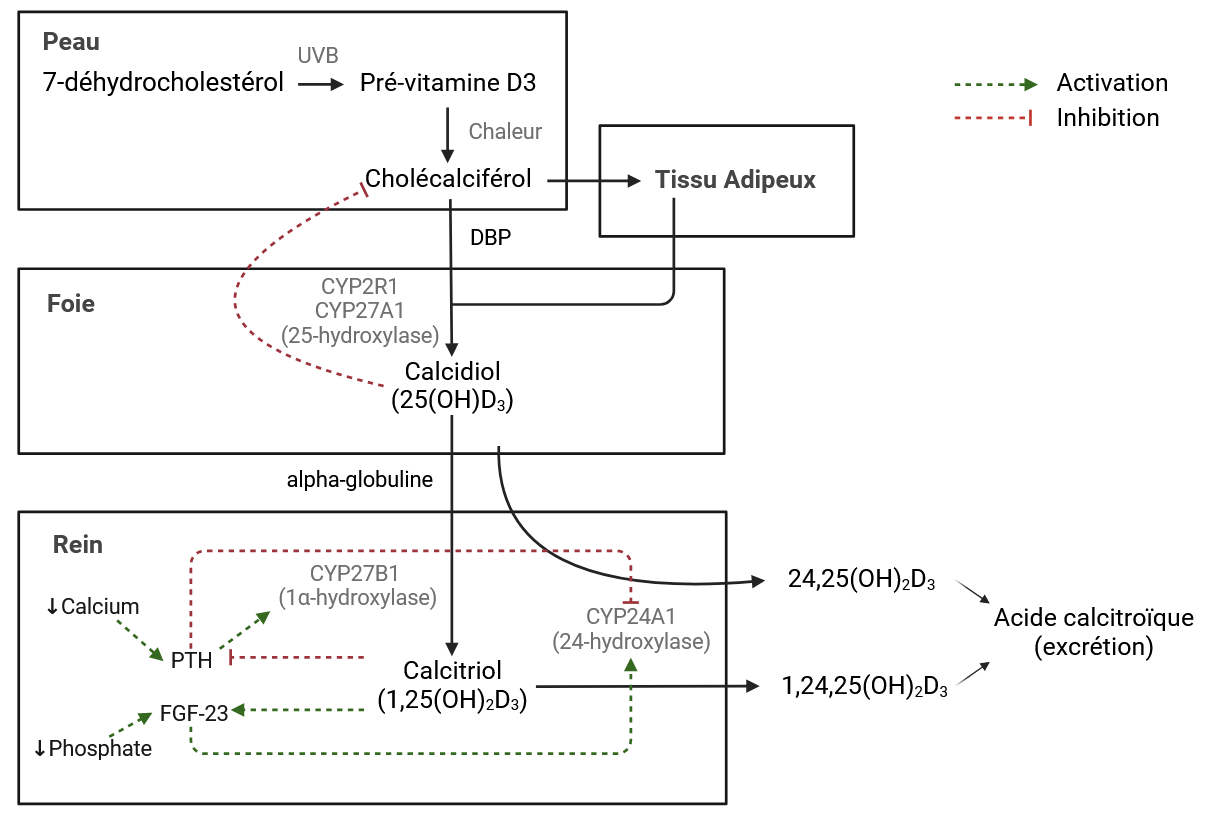
\includegraphics{figures/vitd-metabolism-fr.png}

}

\caption[Métabolisme de la vitamine
D.]{\label{fig-vitd-metabolism}\textbf{Métabolisme de la vitamine D.} Le
métabolisme de la vitamine D débute lorsque le 7-déhydrocholestérol
présent dans la peau, est transformé par les rayons ultraviolets
provenant du soleil en cholécalciférol. Le cholécalciférol ou vitamine
D\textsubscript{3} est ensuite transporté par la protéine de liaison à
la vitamine D, et est métabolisé dans le foie par des enzymes
25-hydroxylases telles que le CYP2R1 en calcidiol ou
25(OH)D\textsubscript{3}. L'autre étape de du métabolisme se situe dans
le rein, où après transport du calcidiol, celui-ci se retrouve
métabolisé en calcitriol ou 1,25(OH)2D\textsubscript{3} par le CYP27B1.
Le calcitriol augmente la concentration de l'hormone de croissance des
fibroblastes 23 \acsu{FGF23} et l'absorption du calcium et diminue la
concentration d'\acf{PTH}, tandis que ceux-ci exercent un rétrocontrôle
négatif sur la concentration de calcitriol, en inhibant directement ou
indirectement la 1α-hydroxylase, ce qui va diminuer la formation de
calcitriol. Lorsque la PTH et le FGF23 sont stimulés lorsque la calcémie
et la phosphatémie est basse respectivement, ce qui va engendrer des
régulations métaboliques permettant de synthétiser d'avantage de
calcitriol afin de réguler le niveau de calcium et de phosphate. D'après
\textcite{Christakos.2010}, \textcite{Tsiaras.2011} et
\textcite{Dankers.2017}}

\end{figure}%

La synthèse du calcitriol est régulée par deux hormones, l'\acf{PTH} et
l'hormone de croissance des fibroblastes 23 (\acsu{FGF23}). Le
\ac{FGF23}, induite par une concentration élevée de calcitriol et une
faible concentration de phosphate dans le sang, favorise l'induction de
la \ac{CYP24A1}, tandis que la \ac{PTH}, induite par une faible
concentration de calcium et inhibée par une forte concentration de
calcitriol, va induire la \ac{CYP24A1} et donc contribuer au catabolisme
du calcitriol \autocite{Dankers.2017,Christakos.2010}. La \ac{PTH} agit
également directement sur les os en augmentant la résorption osseuse et
augmentant ainsi la calcémie.

\section{Place de l'ergostérol}\label{place-de-lergostuxe9rol}

L'ergostérol ou vitamine D2 est une autre forme de vitamine D
(\Cref{fig:ergo-struc}). Les deux formes de vitamine sont perçues comme
interchangeables ; cependant, la vitamine D3 est considérée plus
intéressante en termes de traitement, car son administration est plus
efficace que celle de la vitamine D2 afin d'augmenter la concentration
de calcidiol et donc pour traiter les carences. En effet, la vitamine
D\textsubscript{2}, de nature végétale ou fongique, possède une
structure légèrement différente de la vitamine D\textsubscript{3}.

De ce fait, elle possède une pharmacocinétique différente, où l'étape de
métabolisation est fonctionnellement différente entre la vitamine
D\textsubscript{2} et vitamine D\textsubscript{3}. Ainsi, lors du
catabolisme de la vitamine D\textsubscript{2}, la 24-hydroxylation du
25(OH)D\textsubscript{2} et du
1,25(OH)\textsubscript{2}D\textsubscript{2} dans le rein conduit aux
métabolites 24,25(OH)\textsubscript{2}D\textsubscript{2} et
1,24,25(OH)\textsubscript{3}D\textsubscript{2} respectivement. Le
1,24,25(OH)\textsubscript{3}D\textsubscript{2} est inactif à la
différence de son analogue \ac{1,24,25(OH)3D3} qui nécessite une
oxydation supplémentaire afin d'être désactivée, et possède entre autres
une affinité pour le \ac{VDR} (jusqu'à 40\% plus forte que
\ac{1,25(OH)2D3}). De plus, la 24-hydroxylation pourrait également avoir
lieu dans le foie, conduisant à la formation de
24(OH)D\textsubscript{2}. Le métabolite en résultant, la
1,24(OH)\textsubscript{2}D2, est moins affin pour le \ac{VDR} comparé à
son analogue D\textsubscript{3}. En revanche, la vitamine
D\textsubscript{3} ne se subit pas cette première 24-hydroxylation
hépatique \autocite{Houghton.2006}.

\begin{figure}

\includegraphics{figures/ergo_vs_chole.png} 
\caption[Comparaison de la structure de l'ergocalciférol par rapport au cholécalciférol.]
{\textbf{Comparaison de la structure de l'ergocalciférol par rapport au cholécalciférol.} La structure de l'ergocalciférol comprend une double liaison et un groupement méthyl (CH\textsubscript{3}) supplémentaire par rapport au cholécalciférol. Cela implique une voie de métabolisation différente, notamment une voie d'élimination plus rapide, et donc une diminution de la concentration en métabolite biologiquement actif issue de l'ergocalciférol. (\cite{Houghton.2006})}
\label{fig:ergo-struc}
\end{figure}

Ainsi, cette différence de structure cause une différence dans
l'évolution de la concentration de 25(OH)D. Une expérience consistant en
une administration d'une dose de 50 000 UI pour les deux types de
vitamine D permet de comparer l'évolution des concentrations respectives
en 25(OH)D (\Cref{fig-PK}). La vitamine D\textsubscript{2} est
inférieure à la vitamine D\textsubscript{3} concernant le maintien d'une
concentration adéquate de 25(OH)D, puisqu'elle s'élimine beaucoup plus
rapidement, malgré une phase d'absorption identique les trois premiers
jours. On observe ainsi qu'au jour 14, la concentration de 25(OH)D
obtenue par ergostérol est redevenue identique à celle au jour 1, tandis
que celle obtenue par vitamine D\textsubscript{3} continue de croître
\autocite{Armas.2004}.

\begin{figure}

\centering{

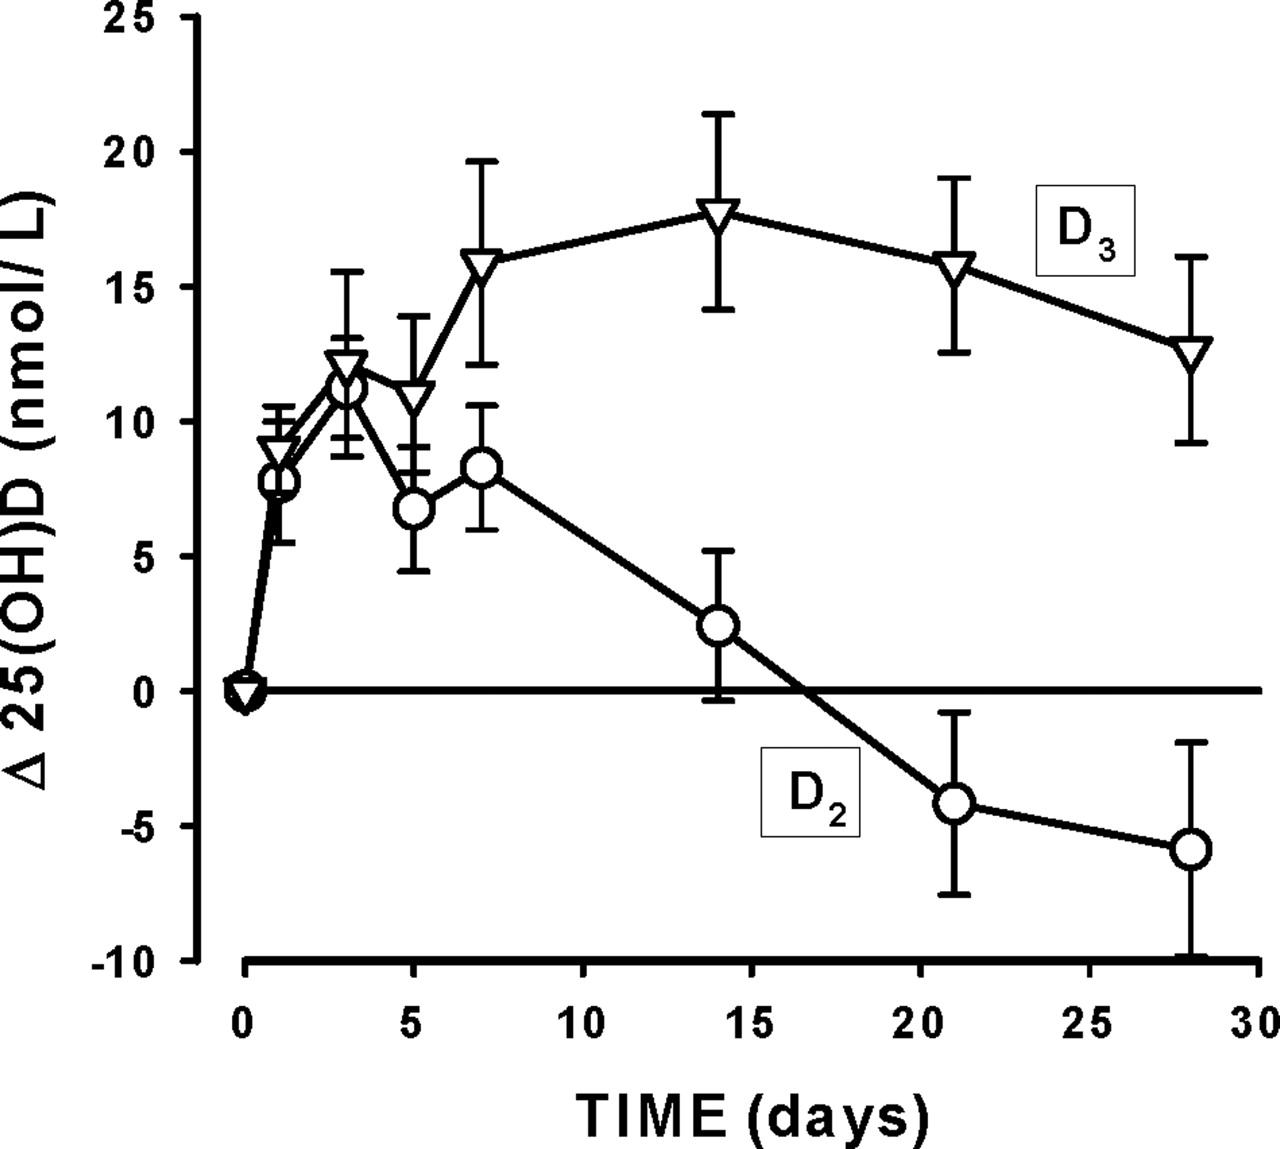
\includegraphics{figures/PK_D2_vs_D3.jpeg}

}

\caption[Evolution de la concentration en 25(OH)D après administration
d'une dose de 50 000 UI de vitamine D\textsubscript{2} ou
D\textsubscript{3} chez 10 patients.]{\label{fig-PK}\textbf{Evolution de
la concentration en 25(OH)D après administration d'une dose de 50 000 UI
de vitamine D\textsubscript{2} ou D\textsubscript{3} chez 10 patients.}
\autocite{Armas.2004}}

\end{figure}%

Ainsi, la vitamine D\textsubscript{3} est généralement capable
d'augmenter la concentration en 25(OH)D environ deux fois plus qu'avec
la vitamine D\textsubscript{2}, comme le montre \textcite{Trang.1998}
lors d'une comparaison avec une dose unique de 4000 UI. Une comparaison
de l'aire sous la courbe entre les deux formes montre un potentiel 3
fois plus important chez la vitamine D\textsubscript{3}
\autocite{Armas.2004}.

L'ergocalciférol continue d'être généralement encore utilisée en tant
que supplément aux Etats-Unis \autocite{Houghton.2006}. Cependant, cette
forme de traitement reste moins efficace voire est insuffisante pour
corriger les déficiences en vitamine D comparé au cholécalciférol, comme
le montre certains essais cliniques \autocite{Boyle.2005}.

Le cholécalciférol étant une forme de vitamine D possédant une meilleure
capacité à augmenter la concentration de vitamine D au long terme, elle
devrait être privilégiée lors de supplémentations. Pour ces raisons,
nous ne discuterons seulement que de la vitamine D\textsubscript{3}
lorsque nous examinerons l'usage et le potentiel thérapeutique de la
vitamine D.

\section{Propriétés}\label{propriuxe9tuxe9s}

\subsection{Propriétés classiques
osseuses}\label{propriuxe9tuxe9s-classiques-osseuses}

L'usage de la vitamine D par le biais de l'huile de foie de morue a été
décrite dans la littérature au plus tôt par Thomas Percival en 1782, qui
rapporte son usage et les effets bénéfiques constatés sur le rhumatisme
chronique en Angleterre \autocite{Percival.1782}. A cette époque,
plusieurs cas de rachitismes causent des morts inexpliquées, le
rachitisme étant une maladie caractérisée par le ramollissement et
l'affaiblissement des os. En France, Armand Trousseau publie dans
l'ouvrage de 1844 du Bulletin général de thérapeutique sur l'utilisation
de l'huile de foie de morue par Armand Trousseau pour le traitement du
rachitisme \autocite{bulletin.label.1844}. Il publie également son
ouvrage Clinique Médicale de l'Hôtel-Dieu en 1861, où il déclare que le
rachitisme est causé par une alimentation déséquilibrée que l'huile de
foie de morue peut résoudre \autocite{Hernigou.2019}.

Dans les années 1917--1922, les progrès concernant les causes et le
traitement du rachitisme se sont accélérées. \textcite{Hess.1917.lc}
démontrent que l'administration de l'huile de foie de morue permet de
prévenir et guérir du rachitisme chez les enfants afro-américains à New
York. En 1918, Mellanby a montré qu'il pouvait prévenir le rachitisme
expérimental chez les chiots avec de l'huile de foie de morue et a
discuté du rôle d'un ``facteur accessoire'' dans la production du
rachitisme \autocite{ORiordan.2014}. Par la suite, \textcite{Hess.1921}
ont rapporté que l'exposition au soleil permettait de guérir du
rachitisme. Ce sera \textcite{McCollum.1922} qui donnera le nom de
Vitamine D au ``facteur accessoire'' proposé par Mellanby
\autocite{Hernigou.2019,Mavrotas.2021}

L'intérêt pour la vitamine D s'est ensuite accru avec la découverte par
les scientifiques de son rôle crucial dans le métabolisme du calcium et
du phosphore. Depuis lors, de nombreuses études ont été menées pour
évaluer le rôle de la vitamine D dans le métabolisme osseux, et il est
désormais largement admis que la vitamine D joue un rôle essentiel dans
le maintien de la santé des os et des dents
\autocite{IOM.2011,Goltzman.2018}. Une carence en vitamine D est
associée à un risque accru d'ostéomalacie (une affection qui entraîne
une diminution de la masse osseuse) et d'ostéoporose (une affection
caractérisée par une fragilité des os).

L'action de la vitamine D est médiée par la liaison du calcitriol, au
récepteur \ac{VDR} \autocite{Norman.2008,Dankers.2017}. La vitamine D
agit directement sur le renouvellement osseux mais joue également un
rôle dans l'homéostasie du calcium. L'homéostasie du calcium dépend de
son absorption dans l'intestin, de sa réabsorption dans le rein et de
fixation/libération dans l'os. Le calcium est absorbé grâce à des
transporteurs transcellulaires (actifs) et paracellulaires (passifs),
grâce au signalement du calcitriol. Celui-ci est considéré comme le
principal facteur régulateur de l'absorption intestinal de calcium.
Lorsque les flux de calcium sont déséquilibrés, les os servent de
réservoir de calcium afin de maintenir l'équilibre calcique. La
réabsorption du calcium par le rein est contrôlée dans le tubule
contourné distal par l'action du calcitriol sur le \ac{VDR}
\autocite{Carmeliet.2015}. Ainsi, la vitamine D joue un rôle crucial
dans l'absorption intestinale du calcium et du phosphore, assurant ainsi
l'homéostasie des niveaux calciques et phosphoriques dans l'organisme.

De plus, la liaison du calcitriol sur le VDR situé dans les ostéoblastes
entraîne une augmentation de la minéralisation osseuse et donc de la
fixation du calcium dans les os (diminution de RANKL, facteur de
transcription activant les ostéoclastes, et augmentation de LRP5)
\autocite{Carmeliet.2015}. Lorsque la calcémie est basse, l'augmentation
de \ac{PTH} conduit à une augmentation de RANKL ce qui favorise la
résorption des os par les ostéoclastes afin d'obtenir du calcium
(\Cref{fig-vitd-metabolism}).

\subsection{Propriétés
extra-osseuses}\label{propriuxe9tuxe9s-extra-osseuses}

La découverte des propriétés extra-osseuses de la vitamine D a commencé
avec le clonage du récepteur \ac{VDR} en 1987. Son identification dans
la majorité des tissus et populations cellulaires a a ouvert la voie à
de nombreuses études fondamentales et cliniques autour du rôle
pléiotrope de la vitamine D \autocite{Rosen.2012}. Le \ac{VDR} est
exprimé de façon ubiquitaire ; cependant, certaines cellules ou tissus,
tels que les globules rouges, les muscles striés, et certaines cellules
hautement différenciés du cerveau telles que les cellules de Purkinje du
cervelet, n'expriment que faiblement \ac{VDR} \autocite{Bouillon.2008}.

Plus récemment l'intérêt pour la vitamine D a été étendue à différentes
pathologies diversement associées à des désordres osseux, en particulier
dans le cancer, les maladies cardio-métaboliques (obésité et diabète de
type 2, métabolisme du glucose) et les maladies auto-immunes (diabète de
type 1, sclérose en plaques, troubles thyroïdiens auto-immuns)
\autocite{Dankers.2017,Caprio.2017}. En effet, plusieurs recherchent
suggèrent que la vitamine D joue un rôle dans le diabète de type 2, en
stimulant l'expression des récepteurs à l'insuline et en augmentant la
sensibilité à l'insuline. Elle jouerait aussi un rôle dans l'obésité au
niveau du tissu adipeux, où des corrélations inverses ont été observées
entre le taux de calcidiol et la leptine (hormone régulant l'appétit) et
résistine (hormone pro-inflammatoire et contribue à la résistance à
l'insuline), et une association positive avec l'adiponectine (hormone
augmentant la sensibilité à l'insuline)
\autocite{Caprio.2017,Bellia.2013}. Il existe une association inverse
entre le taux de calcidiol et de marqueurs d'inflammation systémique
observée chez les sujets obèses \autocite{Bellia.2013}. En ce qui
concerne les bénéfices liés à l'immunité, les effets observés de la
vitamine D sont généralement associés à une régulation négative de
l'inflammation, par l'inhibition de \ac{CMH-II}, des molécules de
co-stimulation, une diminution de l'activité des Th\textsubscript{1} et
Th\textsubscript{17}, lymphocytes pro-inflammatoires, et une
augmentation des T\textsubscript{regs}, lymphocytes anti-inflammatoires
(\Cref{fig:extra-skeletal}). Un autre domaine d'intérêt concernant les
effets extra-squelettiques de la vitamine D concerne son rôle au niveau
des muscles squelettiques. Plusieurs études suggèrent que le rôle de la
vitamine D stimule la synthèse des protéines musculaires ainsi que la
réabsorption du calcium dans le réticulum sarcoplasmique, ce qui permet
de maintenir une force musculaire adéquate\autocite{Caprio.2017}.

\begin{landscape}
\begin{figure}
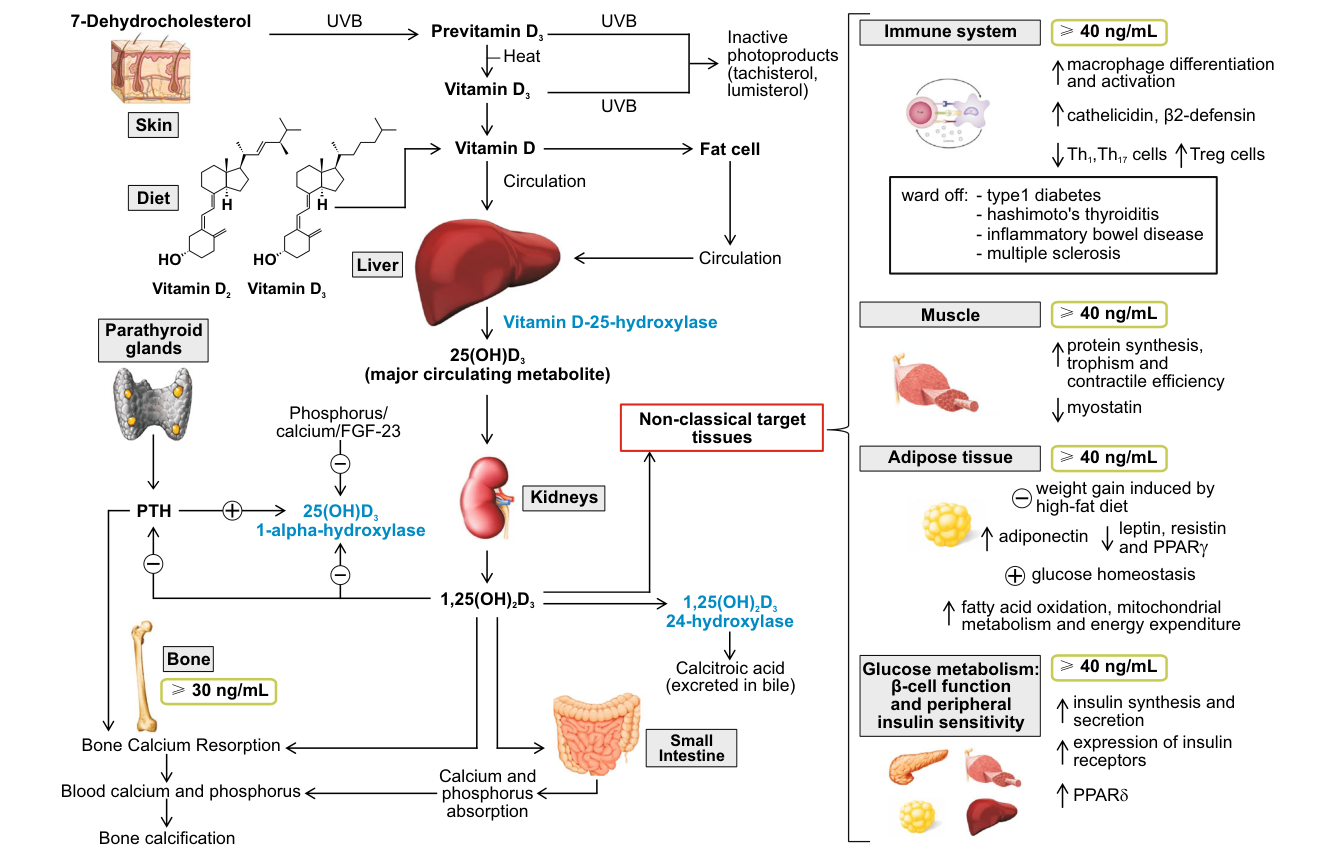
\includegraphics{figures/extra-skeletal-effect.png} 
\caption[Effets classiques et extra-squelettiques de la vitamine D.]
{Effets classiques et extra-squelettiques de la vitamine D. \textcite{Caprio.2017}}
\label{fig:extra-skeletal}
\end{figure}
\end{landscape}

La vitamine D exerce en plus de son action endocrine classique,
dépendante de la 1-hydroxylation par le rein, une action locale
autocrine et paracrine, par le biais d'une expression locale de
l'hydroxylase \ac{CYP27B1} dans différents tissus
\autocite{Carmeliet.2015,Cannell.2008}. Cela concerne notamment les
mécanismes d'action de la vitamine D liés à l'immunité.

Cependant, les bénéfices extra-squelettiques associés à la vitamine D ne
seraient visibles que lorsque la concentration de calcidiol serait
supérieure au seuil de 20-30 ng/mL actuellement recommandé par les
autorités. Le seuil exact de bénéfice accru reste spéculatif à cause de
rapports contradictoires sur la supplémentation en vitamine D issus des
études cliniques randomisées \autocites[ ]{Caprio.2017}[
]{Lewis.2015}{Bouillon.2013,Rejnmark.2017}.

\section{Doses thérapeutiques
efficaces}\label{doses-thuxe9rapeutiques-efficaces}

\subsection{Unités}\label{unituxe9s}

L'expression de la dose de la vitamine D peut se faire en plusieurs
unités. Classiquement, c'est l'\ac{UI} qui est utilisée. Elle peut
également être exprimée en masse lors de prises de comprimés.
L'équivalence est de 1 µg pour 40 \ac{UI} ou 1 \ac{UI} pour 0,025 g. La
concentration de vitamine D (en fait celle de calcidiol utilisée comme
marqueur du statut vitaminique) est définie en ng/mL ou en nmol/L. Pour
passer de ng/mL en nmol/L, il suffit de multiplier par 2.5
\autocite{Pramyothin.2012}

Cependant la \ac{FDA} a décidé depuis janvier 2021 de passer à une dose
écrite en microgramme, ce qui oblige les fabricants à donner
l'information en microgramme, bien que la dénomination en UI reste
possible en parallèle \autocite{HHS.2016}.

Un essai-clinique visant à établir l'efficacité de la supplémentation en
cholécalciférol selon trois différents temps d'administration de la
vitamine D a été réalisée sur 61 patients, en divisant les patients en
trois groupes, selon la prise de 1000 UI par jour, 7000 UI par semaine
ou 30 000 UI par mois de vitamine D. Les patients sélectionnés sont
carencés avec une concentration de vitamine D inférieure à 20 ng/mL (en
moyenne autour de 13,3 ng/mL) et ont été suivi pendant 3 mois. L'étude a
permis de déterminer qu'en moyenne, une supplémentation en
cholécalciférol augmente la concentration de calcidiol de 1.3 ng/100 UI
par jour \autocite{Takács.2017}.

\subsection{Dose recommandée
journalière}\label{dose-recommanduxe9e-journaliuxe8re}

Actuellement, l'Académie de médecine américaine (anciennement Institute
of Medecine, \acsu{IOM}) est responsable des recommandations émises par
la \ac{FDA}, l'équivalent de l'\ac{ANSM} en France. L'\ac{AJR} pour la
vitamine D est de 600 UI par jour pour les personnes tous sexes
confondus de 1 à 70 ans, et reste la même en cas de grossesse ou
d'allaitement \autocite{IOM.2011}. L'\ac{AJR} est augmentée à 800
UI/jour chez les personnes de plus de 70 ans en raison de la plus grande
variance des données disponibles concernant cette catégorie d'âge. Une
concentration sanguine de calcidiol de 20 ng/mL ou plus est considérée
par l'\ac{IOM} comme étant le minimum adéquat chez 97,5 \% des personnes
en bonne santé. Cette concentration minimum de 20 ng/mL a été observé
comme étant bénéfique pour la santé osseuse concernant la majorité de la
population générale, se manifestant par une augmentation de la densité
minérale osseuse et de l'absorption du calcium, de l'accrétion osseuse
et de la maintenance osseuse, diminution de l'ostéomalacie et de
rachitisme. Les concentrations de calcitriol supérieures à 30 ng/mL ne
sont pas associées à une augmentation de ces bénéfices considérés selon
l'\ac{IOM} \autocite{IOM.2011,Rosen.IOM.2012}.

Un autre acteur français, l'\ac{ANSES}, stipule que les recommandations
journalières de cholécalciférol sont de 15 µg par jour pour un adulte,
soit l'équivalent d'une dose de 600 UI/j, s'appuyant sur les
recommandations de l'Autorité européenne de sécurité des aliments
(\acsu{EFSA}) \autocite{ANSES.2021}. En effet, l'\ac{EFSA} a retenu une
valeur de 15 µg/j (soit 600 UI/j) permettant aux hommes et femmes
d'atteindre le seuil de calcitriol jugé adéquat de 50 nmol/L ou 20 ng/mL
\autocite{ANSES.2022.note} (\Cref{tbl-seuil}).

\begin{table}
\caption[Tableau comparatif des seuils d'adéquation de la vitamine D par différentes sources.]{Tableau comparatif des seuils d'adéquation de la vitamine D par différentes sources. IOM : Institut de Médecine ; ANSES : Agence nationale de sécurité sanitaire de l’alimentation, de l’environnement et du travail. D'après \textcite{IOM.2011} et \textcite{ANSES.2021}}
\label{tbl-seuil}
\centering
\begin{tabular}{ccc}
\toprule
\textbf{Seuil de vitamine D} & \textbf{IOM} & \textbf{ANSES}\\
\midrule
Déficience en vitamine D & < 12 ng/mL & < 10 ng/mL\\
Insuffisance en vitamine D & 12-20 ng/mL & 10-20 ng/mL\\
Valeurs recommandées & 20-30 ng/mL & 20-30 ng/mL\\
Limite Supérieure de Sécurité & > 50 ng/mL  & > 100 ng/mL \\
\bottomrule
\end{tabular}
\end{table}

\begin{table}
\centering
\caption[{Apports journaliers recommandés de la vitamine D (UI/j)}]{\textbf{Apports journaliers recommandés de la vitamine D (UI/j).} La mention de \ac{AJR} indique que l'apport couvre les besoins minimes de 97.5\% de la population pour une concentration de 20 ng/mL selon l'\ac{IOM}. D'après \textcite{ANSES.2021, IOM.2011}}
\label{tbl-AJR}
\begin{tabular}{ccc}
\toprule
\textbf{Groupe d'âge} & \textbf{IOM} & \textbf{ANSES/EFSA} \\
\midrule
Nourrissons (0-12 mois) & 400 & 400 \\
Enfants (1 - 11 ans) & 600 & 600 \\
Adolescents (11 - 17 ans) & 600 & 600 \\
Hommes et Femmes & 800 & 600 \\
Femmes enceintes & 600 & 600 \\
\bottomrule
\end{tabular}
\end{table}

\subsection{Controverse autour de la dose recommandée
journalière}\label{controverse-autour-de-la-dose-recommanduxe9e-journaliuxe8re}

Plusieurs acteurs tels que la Société d'Endocrinologie suggèrent que
l'\ac{AJR} établi par l'\ac{IOM} est insuffisante. La Société
d'Endocrinologie suggère un \ac{AJR} de 1500 UI/j pouvant aller à 2000
UI/j pour des adultes, avec des recommandations ciblées pour des
populations à risque avec des maladies spécifiques visant un seuil jugé
optimal de 30 ng/mL. L'\ac{IOM} suggère dans une réponse à la Société
d'Endocrinologie que les auteurs ont fait un amalgame entre apports
nutritionnels pour la population générale et l'établissement des
recommandations pour des personnes à risque, ce qui inclut des
conditions adéquates pour la population générale
\autocite{Rosen.IOM.2012}. De plus, l'\ac{IOM} est en désaccord
concernant les bénéfices osseux, concluant sur la base de la littérature
qu'il n'y a pas de bénéfices osseux observés au-delà de 20 ng/mL, qui
est le seuil permettant de couvrir les besoins minimes de 97.5\% de la
population (\Cref{tbl-seuil}). L'\ac{IOM} conclut que les bénéfices
extra-squelettiques de la vitamine D sont incertains et que les preuves
ne sont pas suffisantes pour recommander une augmentation de l'\ac{AJR}
\autocite{IOM.2011}.

\section{Utilisation thérapeutique}\label{utilisation-thuxe9rapeutique}

La vitamine D est surtout utilisée en thérapeutique afin de prévenir les
carences à des fins de bonne santé osseuse. Elle permet de prévenir le
rachitisme chez les enfants et l'ostéoporose chez les adultes et surtout
chez les personnes âgées. Elle permet de maintenir une bonne densité
osseuse et une absorption du calcium adéquat et prévient du rachitisme
et de l'ostéomalacie.

\section{Pharmacocinétique}\label{pharmacocinuxe9tique}

La pharmacocinétique est l'étude du mouvement d'une substance à travers
les différents systèmes biologiques de l'organisme, et décrit la manière
dont l'organisme affecte une substance spécifique après son
administration. La pharmacocinétique traite des paramètres tels que
l'absorption, la distribution, la biodisponibilité, le métabolisme,
l'excrétion et la toxicité. Elle peut aussi être utilisée pour étudier
l'apparition, la durée et l'intensité de l'effet d'un médicament ainsi
qu'observer la relation entre la dose et la réponse de l'organisme.

La pharmacocinétique de la vitamine D est cependant beaucoup plus
complexe que celle d'un agent pharmacologique standard, en raison de
l'hydroxylation progressive nécessaire pour obtenir sa forme active, et
de la présence de la vitamine D et de ses métabolites dans la
circulation et les tissus. De plus, sa liaison à son transporteur
\ac{DBP} influence les propriétés des métabolites de la vitamine D
\autocite{Schoenmakers.2018}. La vitamine D est hydroxylée dans le
plasma en 25(OH)D par le CYP2R1. Cette enzyme possédant une haute
capacité de métabolisation, la présence de vitamine D non hydroxylée
n'est visible uniquement lorsqu'elle atteint une concentration saturant
cette enzyme \autocite{Schoenmakers.2018}.

La vitamine D (en tant que cholécalciférol) possède une bonne absorption
rapide et linéaire, atteignant la \ac{Cmax} pour une dose de vitamine
D\textsubscript{3} à un \ac{Tmax} de 6 à 10 heures. Le calcidiol est
absorbé plus rapidement que le cholécalciférol, avec un \ac{Tmax} de 4 à
6 heures (\textbf{Figure~\ref{fig-PK-all-VitD}})
\autocite{Schoenmakers.2018}.

La majorité de la vitamine D absorbée est associée à des chylomicrons,
puis est redistribuée vers les protéines plasmatiques comme les
lipoprotéines, et enfin est transférée vers la protéine de transport
principale, la \ac{DBP}. Le calcidiol plasmatique est majoritairement
lié à la DBP à 85\%, 15 \% à l'albumine et 0.03\% sous forme libre. La
vitamine D étant une molécule liposoluble, elle principalement
distribuée dans les tissus adipeux, mais également les tissus
musculaires. Elle se retrouve dans divers autres tissus tels que la
peau, le plasma et d'autres organes. La vitamine D peut varier
considérablement entre 10 à 900 nmol/kg et le calcidiol de 2,3 à 12,8
nmol/kg. Les muscles détiennent autour de 10\%--20\% de la vitamine D
distribuée dans les tissus adipeux où le ratio de calcidiol varie entre
0.5 à 1 en fonction de l'alimentation et du type de fibre musculaire. La
concentration de calcidiol varie entre 75\%--150\% de la vitamine D
présente dans les tissus adipeux \autocite{Schoenmakers.2018}. La
vitamine D étant une molécule liposoluble et se distribuant abondamment
dans les tissus adipeux, il est possible de considérer que ce
compartiment de distribution ait un impact sur la pharmacocinétique de
la vitamine D. Des données récentes suggèrent que la perte de poids
n'influence pas le statut en vitamine D. De plus, il n'est pas certain
que la mobilisation de la vitamine D et de la 25(OH)D repose sur la
diffusion de la forme libre ou liée, ou qu'elle soit régulée, et
l'impact de la masse adipeuse sur la pharmacocinétique de la vitamine D
est encore inconnu \autocite{Schoenmakers.2018}.

Cependant il est connu que la dose de vitamine D à administrer pour
viser un seuil thérapeutique doit augmenter lorsque la masse graisseuse
augmente, puisqu'un des compartiments de distribution est plus grand,
représenté par la masse graisseuse. La relation entre l'\ac{IMC} a été
étudiée par \textcite{Ekwaru.2014}. Ekwaru montre ainsi la relation
dose-réponse entre l'administration orale de cholécalciférol et la
concentration plasmatique de calcidiol (\Cref{subfig:vd-dose-response}),
en distinguant les différentes réponses observées lorsque les sujets
sont classés selon leur \ac{IMC} (\Cref{subfig:vd-dose-imc}). On observe
que les sujets ayant un \ac{IMC} plus élevé ont besoin d'une dose plus
élevée de vitamine D pour atteindre le même seuil de concentration
plasmatique de calcidiol.

Les auteurs observent une relation dose-réponse exponentielle, où
l'augmentation sérique de calcidiol diminue avec l'augmentation des
niveaux de supplémentation orale en vitamine D. Les auteurs notent que
l'\ac{IMC} est un meilleur indicateur que le poids absolu afin de juger
de la quantité de vitamine D à administrer. L'\ac{IOM} confirme
également une relation non linéaire avec une augmentation plus marquée
des taux de calcidiol sérique à des doses inférieures à 1000 UI/j. La
réponse est plus aplatie lorsque les doses sont supérieures à 1000 UI/j
\autocite{IOM.2011,Garland.2011}. De ce fait, l'augmentation en vitamine
D obtenue par supplémentation est moindre lorsque la concentration
initiale de vitamine D est plus élevée (\Cref{fig:vd-expected-rise}).

\begin{figure}
    \centering
    \begin{subfigure}{0.48\textwidth}
        \centering
        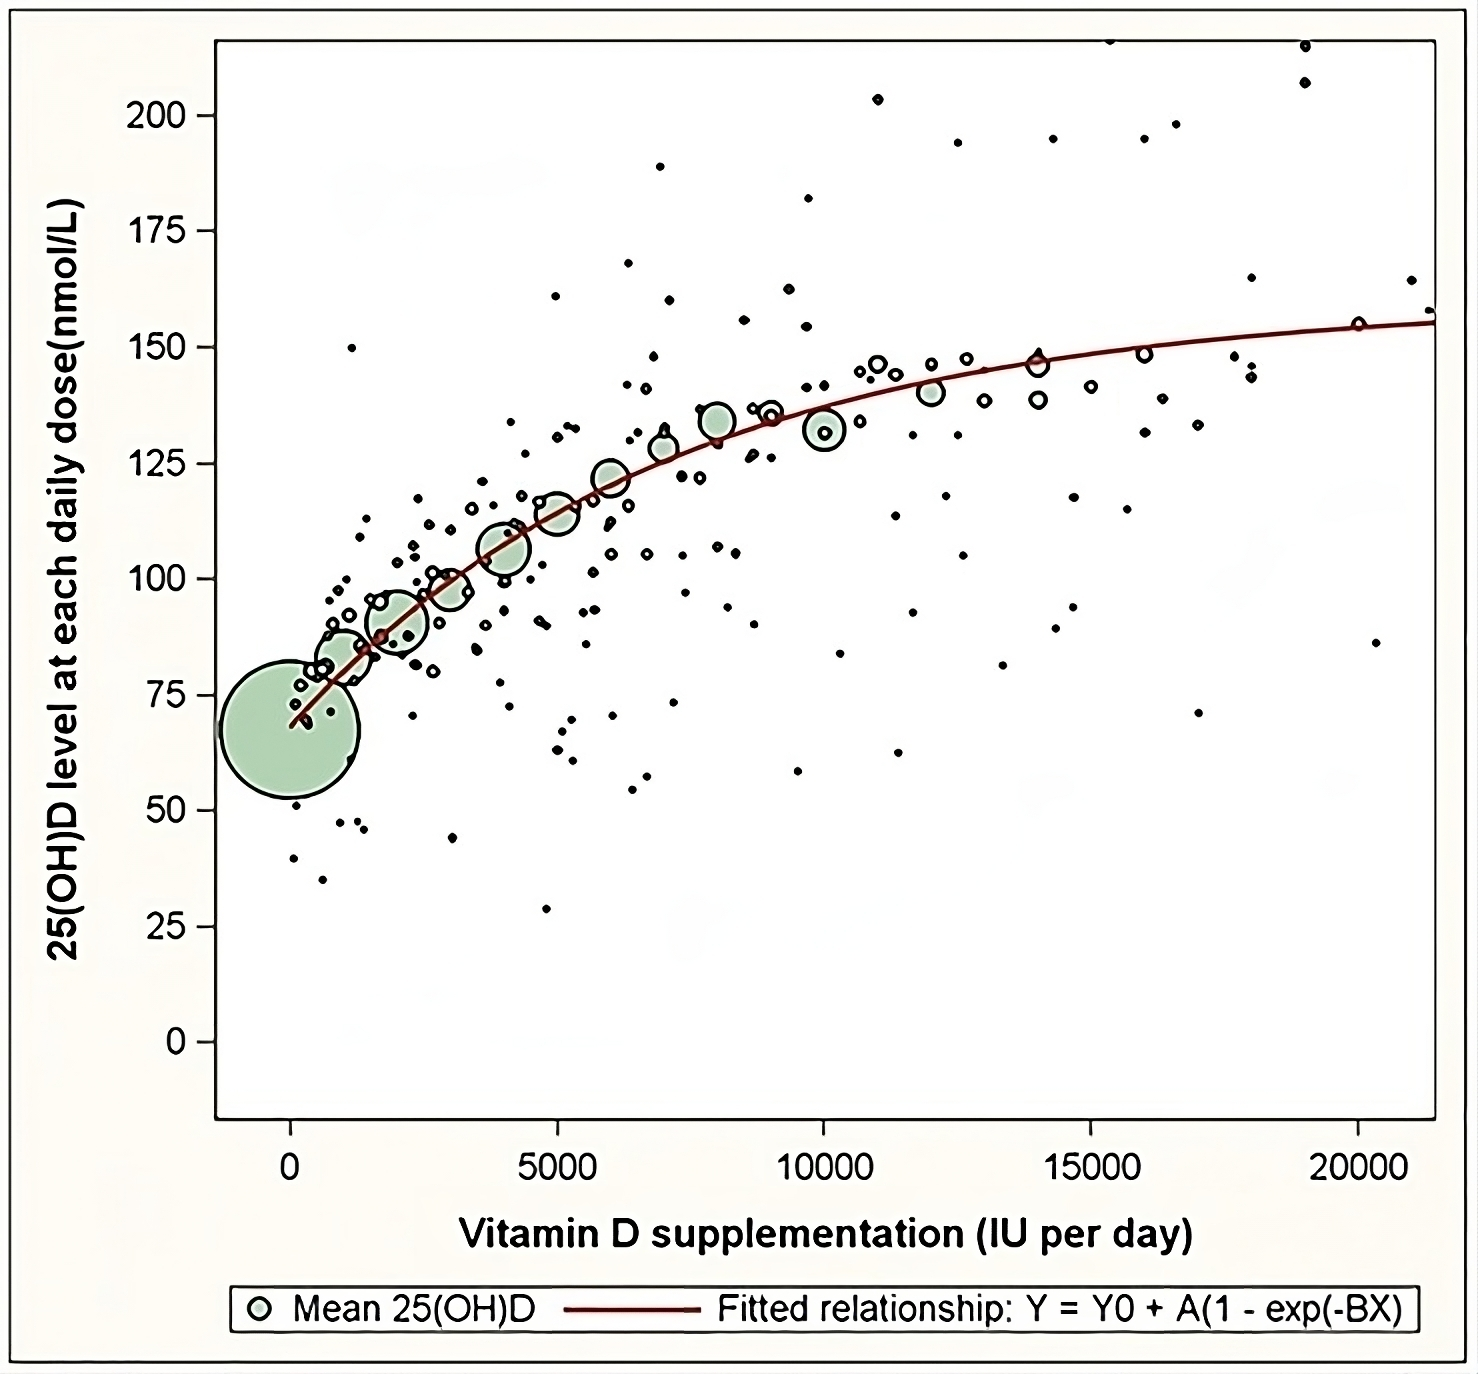
\includegraphics[width=\textwidth]{figures/ekwaru-dose-relation-transformed.jpg}
        \subcaption{Relation dose-réponse entre la prise de cholécalciférol orale et la concentration plasmatique en 25(OH)D \textcite{Ekwaru.2014}.}
        \label{subfig:vd-dose-response}
    \end{subfigure}
    \hfill
    \begin{subfigure}{0.48\textwidth}
        \centering
        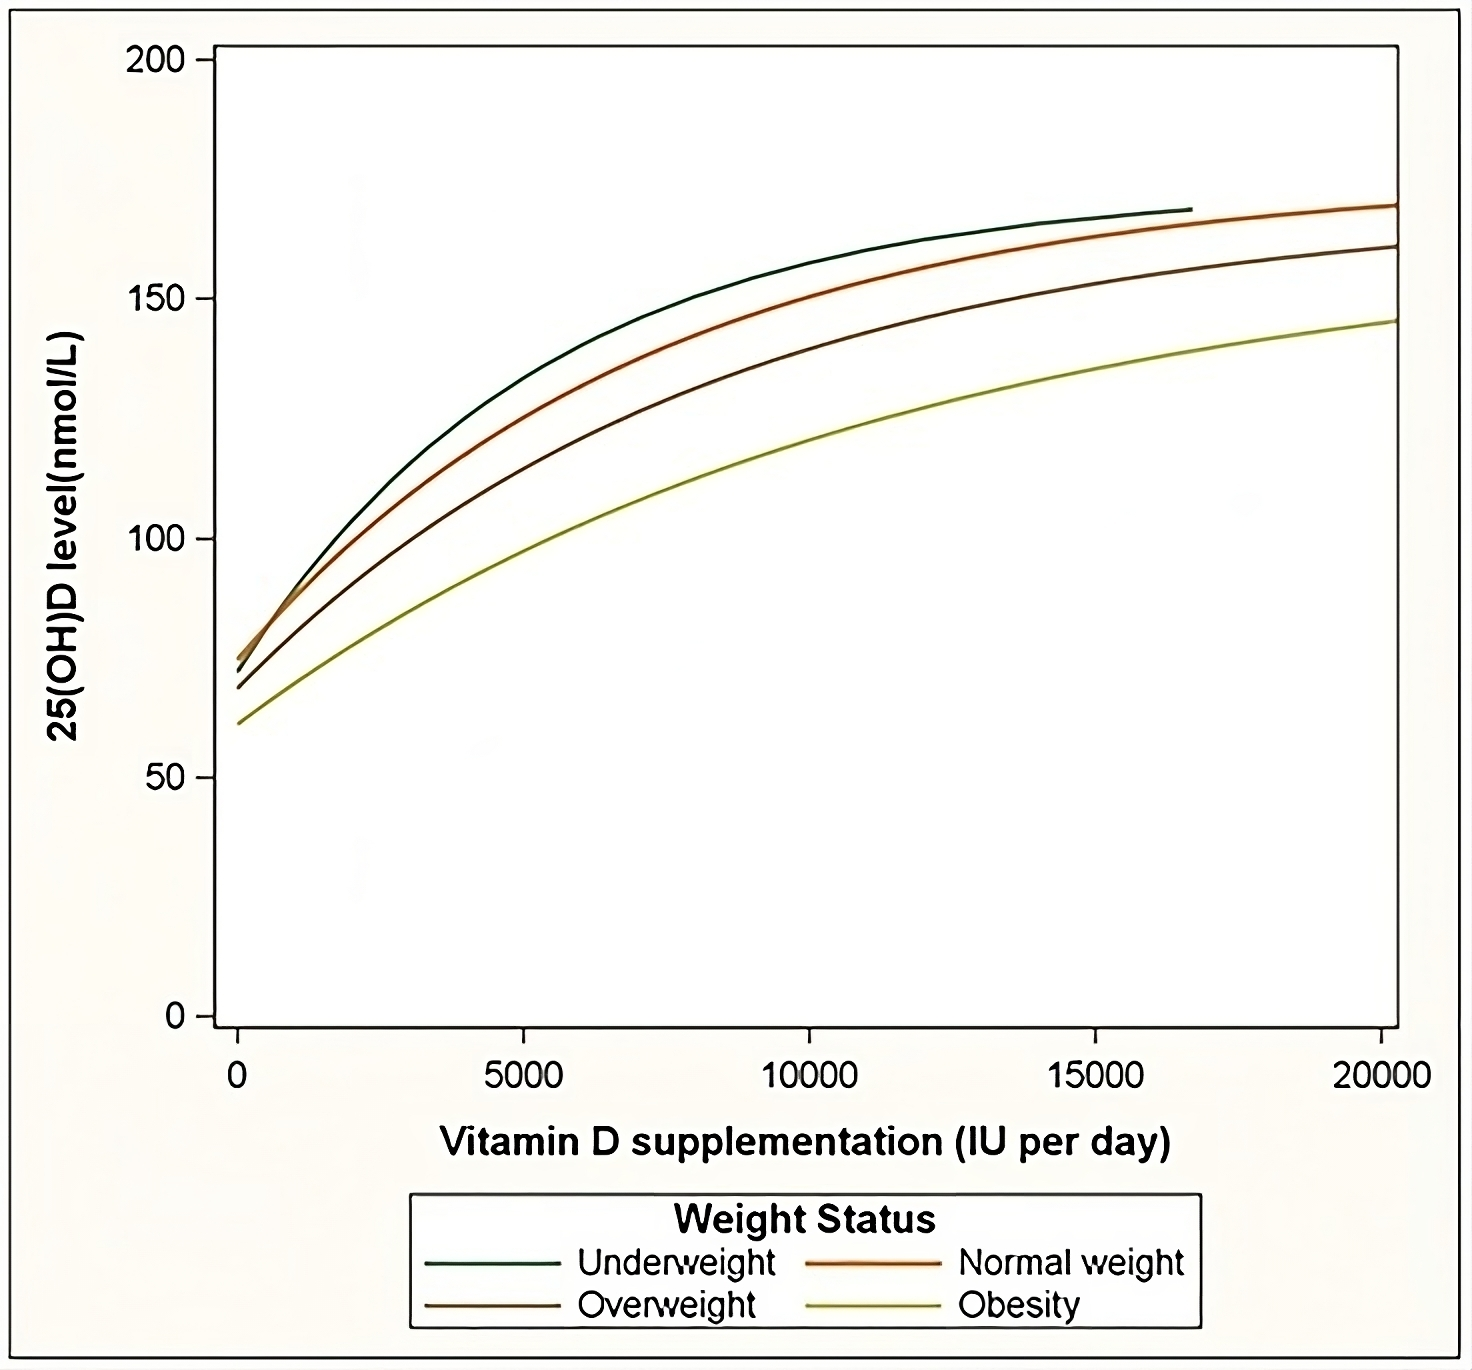
\includegraphics[width=\textwidth]{figures/ekwaru-dose-imc-transformed.jpg}
        \subcaption{Comparaison des courbes dose-réponses entre les différents types de poids déterminé par l'indice de masse corporelle \textcite{Ekwaru.2014}.}
        \label{subfig:vd-dose-imc}
    \end{subfigure}
    \caption[Courbes dose-réponse de la supplémentation en vitamine D orale.]{\textbf{Courbes dose-réponse de la supplémentation en vitamine D orale.}}
    \label{fig:dose-response}
\end{figure}

\begin{figure}
\centering
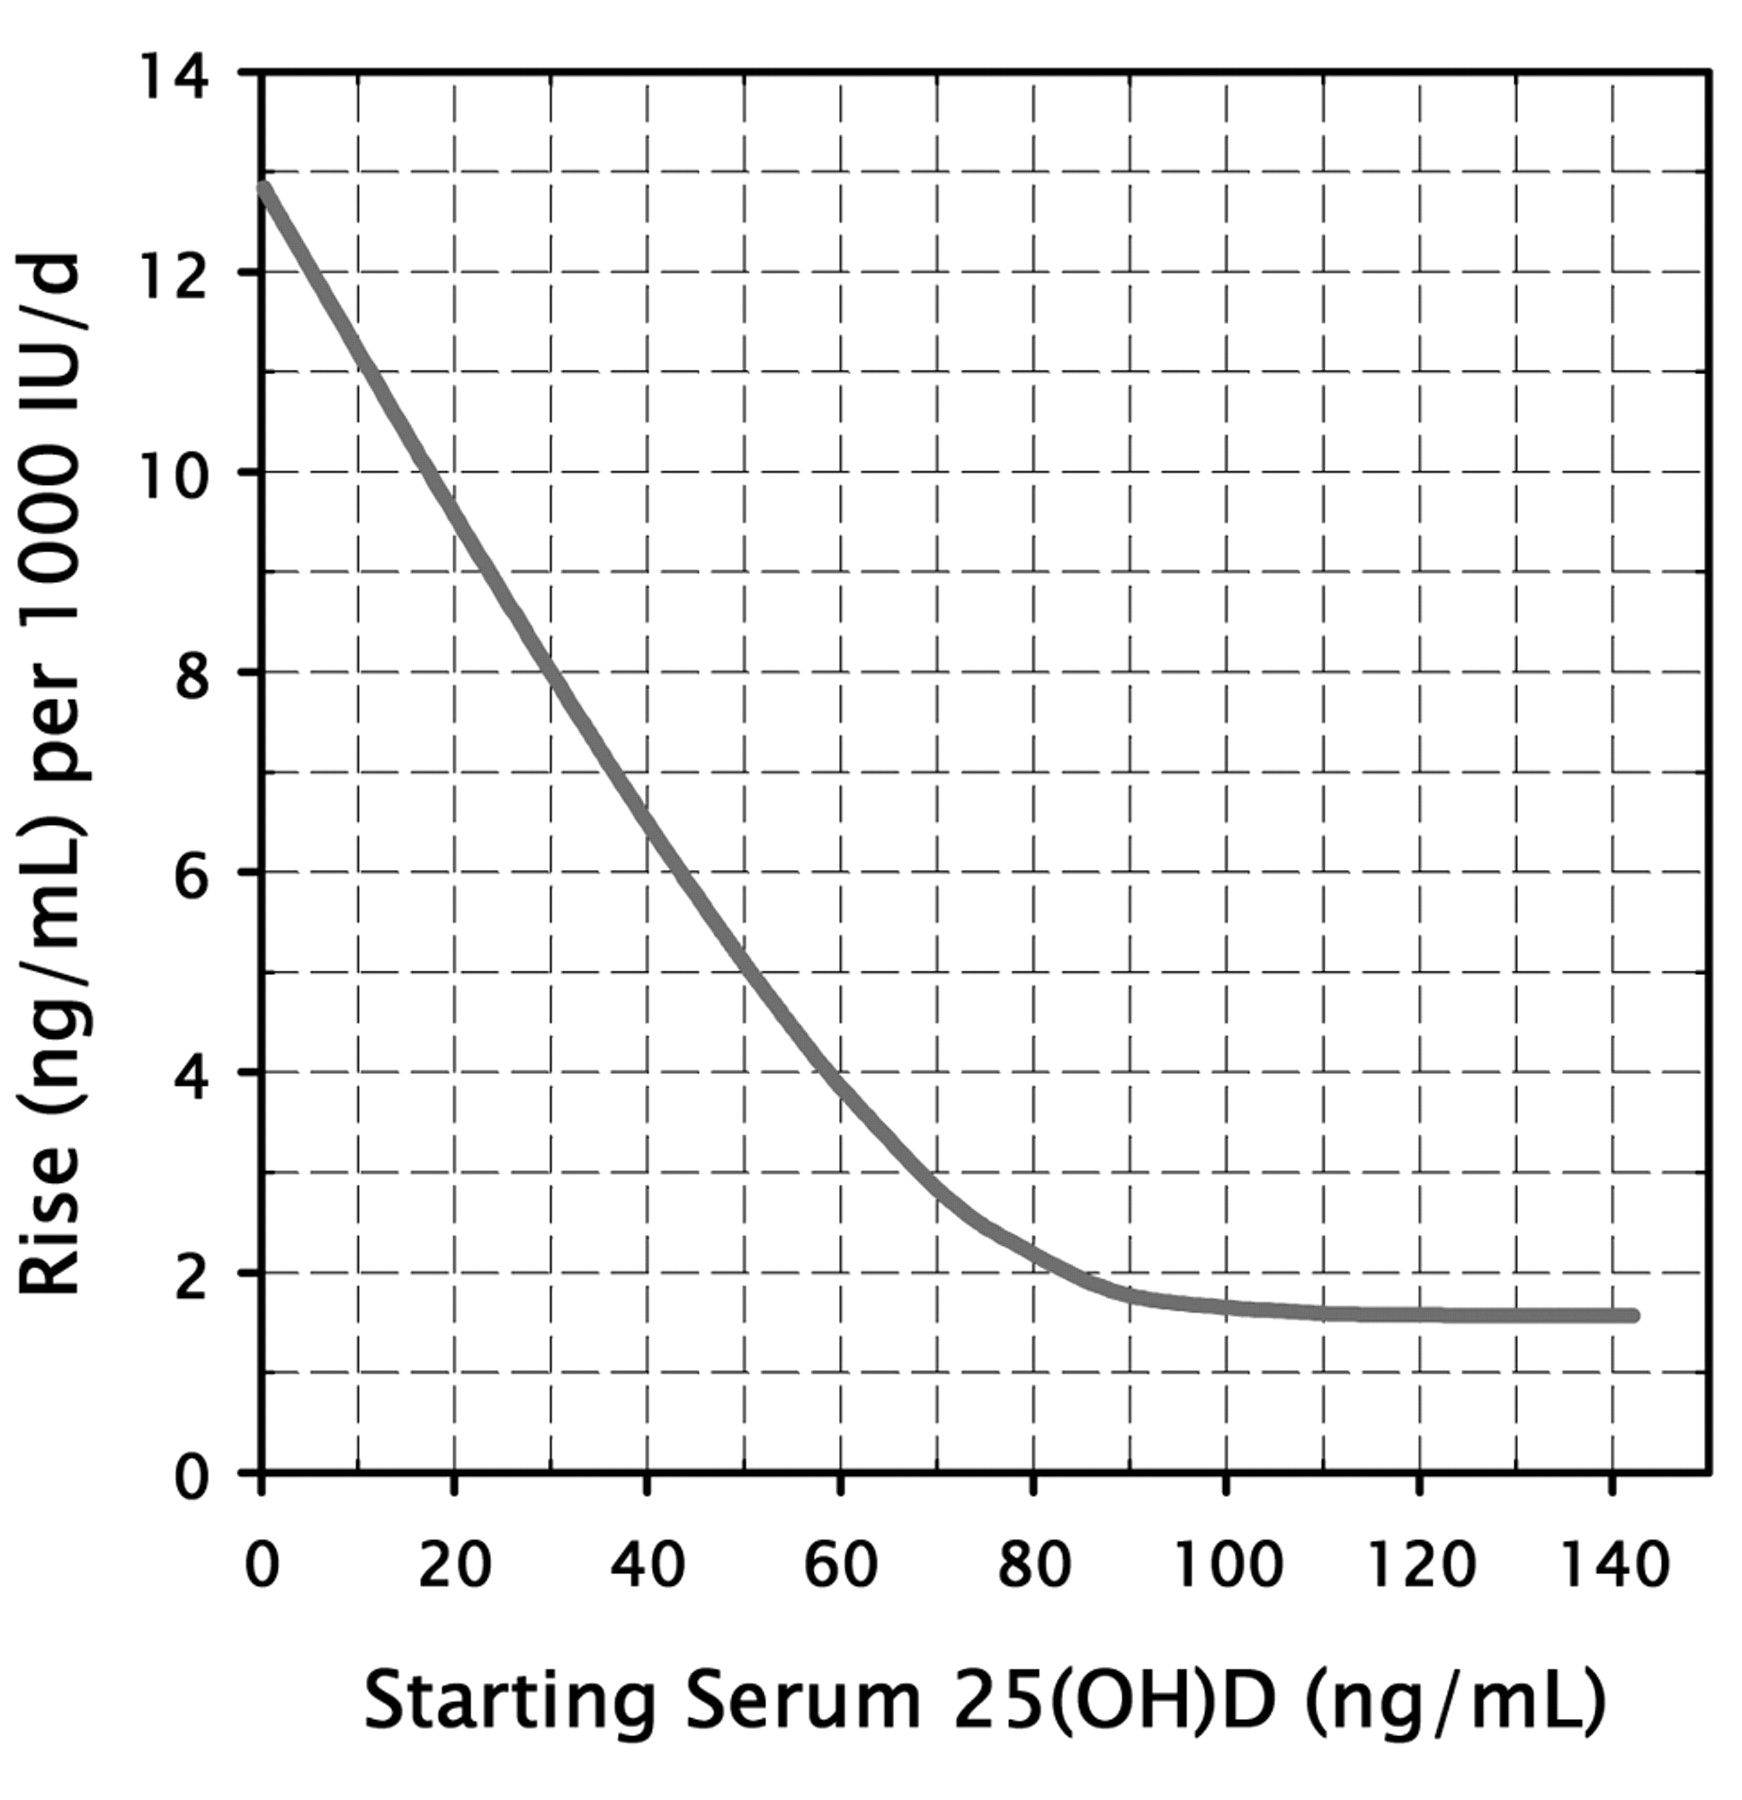
\includegraphics[width=0.5\textwidth]{figures/vd-expected-rise.jpeg}
\caption[Courbe de l'augmentation attendue de la 25(OH)D sérique pour chaque supplément de 1,000 UI de vitamine D3 par jour, en fonction de la valeur de base de la 25(OH)D de base]{\textbf{Courbe de l'augmentation attendue de la 25(OH)D sérique pour chaque supplément de 1,000 UI de vitamine D3 par jour, en fonction de la valeur de base de la 25(OH)D de base.} \textcite{Garland.2011}.}
\label{fig:vd-expected-rise}
\end{figure}

La demi-vie du cholécalciférol est de 24 heures, et celle du calcidiol
est de 10-40 jours, tandis que le calcitriol possède une très courte
demi-vie comparativement, d'une durée de 5-80 heures. Le métabolite
24,25(OH)2D possède quant à lui une demi-vie de 7-16 jours
\autocite{Schoenmakers.2018}. On observe ainsi que la vitamine D est
absorbée très rapidement, et se distribue rapidement dans les tissus,
mais que sa demi-vie est très longue, maintenant une concentration
plasmatique stable pendant plusieurs semaines
(\textbf{Figure~\ref{fig-PK-all-VitD}}).

\begin{figure}

\centering{

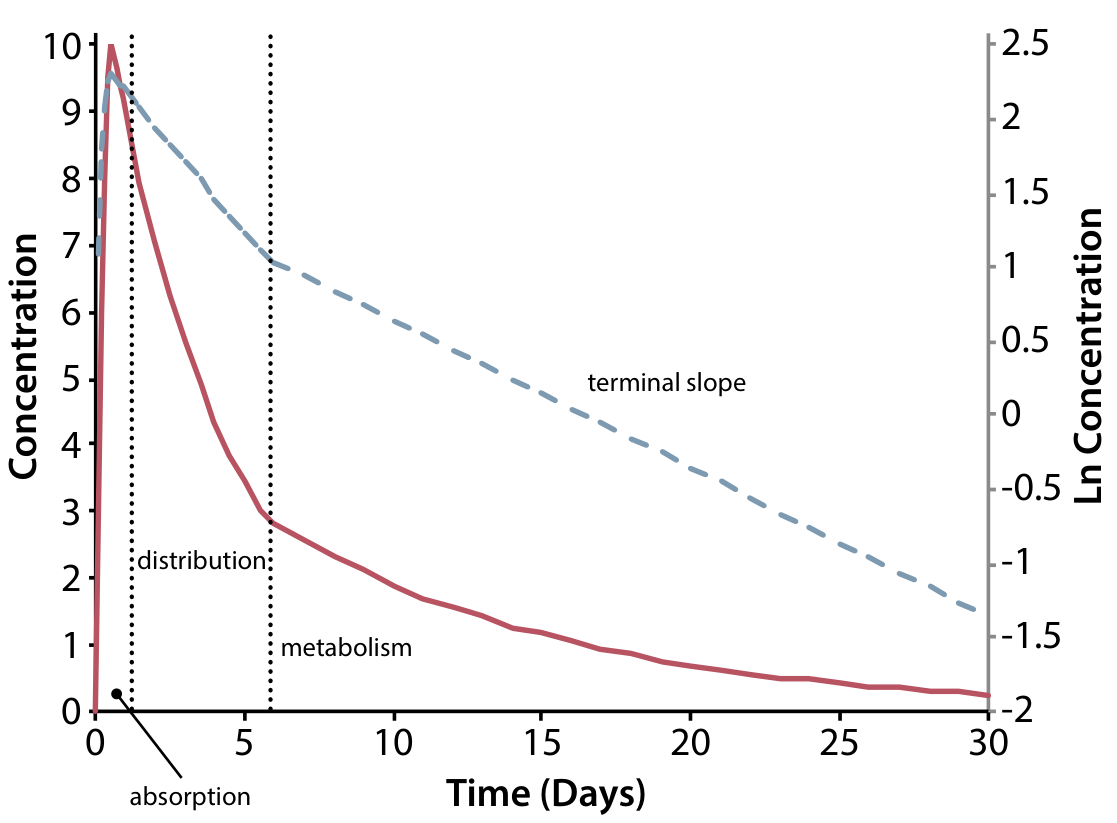
\includegraphics{figures/Schoenmakers.2018 - Plasma appearance and disappearance of 25(OH)D after oral intake.png}

}

\caption[Schéma des phases pharmacocinétiques du
cholécalciférol]{\label{fig-PK-all-VitD}\textbf{Schéma des phases
pharmacocinétiques du cholécalciférol} \autocite{Schoenmakers.2018}}

\end{figure}%

\section{Toxicité}\label{toxicituxe9}

La toxicité de la vitamine D est définie comme un état hypercalcémique
et hypercalciurique qui suggère un excès d'activité lié aux effets du
calcitriol \autocite{Vieth.1990}. Cet état s'accompagne d'une
suppression de l'activité de la \ac{PTH}, en raison de l'état
hypercalcémique qui exerce un rétrocontrôle négatif sur la \ac{PTH}
\autocites[ ]{Marcinowska-Suchowierska.2018}{Dusso.2005}.

La toxicité associée à la vitamine D et de ses métabolites résulte
principalement de l'hypercalcémie et de l'hyperphosphatémie engendrée
lors d'une haute concentration de de vitamine D et de ses métabolites
\autocites[ ]{DeLuca.2011}{Janoušek.2022,Jones.2008,IOM.2011}. Les
premiers symptômes de la toxicité de la vitamine D comprennent donc des
mécanismes causés par cette hypercalcémie, affectant divers organes
(Figure~\ref{fig-hypervitaminose-d}). L'augmentation de cholécalciférol
est corrélée à une augmentation de calcidiol qui peut être amenée à
causer une augmentation de l'absorption du calcium dans l'intestin ainsi
qu'à une résorption osseuse \autocite{Jones.2008,IOM.2011}.
\textcite{Shepard.1980} mentionnent que l'hypercalcémie due à une
hypervitaminose D provient probablement de cette résorption osseuse
plutôt que de l'absorption intestinale accrue du calcium.
(\textbf{Référence compliquée à vérifier} : \textcite{Shepard.1980}
mentionnent ce passage : \emph{Lindquist \autocite{Lindquist.1952} a
montré que la mobilisation du calcium osseux augmente avec la dose
logarithmique, même pour des quantités massives de vitamine D, alors que
la réponse calcique intestinale devient saturée pour des doses très
faibles de vitamine D.}) Des expériences animales ont établi que le
calcidiol peut atteindre des concentrations allant jusqu'à 2,5 mol/L où
l'hypercalcémie est observée \autocite{Jones.2008}.

Les manifestations cliniques de la toxicité associée à la vitamine D
concernent notamment des troubles gastro-intestinaux, des troubles du
système cardiovasculaire ainsi que des troubles du système
musculo-squelettique. Le système rénal est également impacté, et un
trouble neurologique est également possible
(\textbf{Figure~\ref{fig-hypervitaminose-d}}) \autocites[
]{Alshahrani.2013}{Janoušek.2022}.

\begin{figure}

\centering{

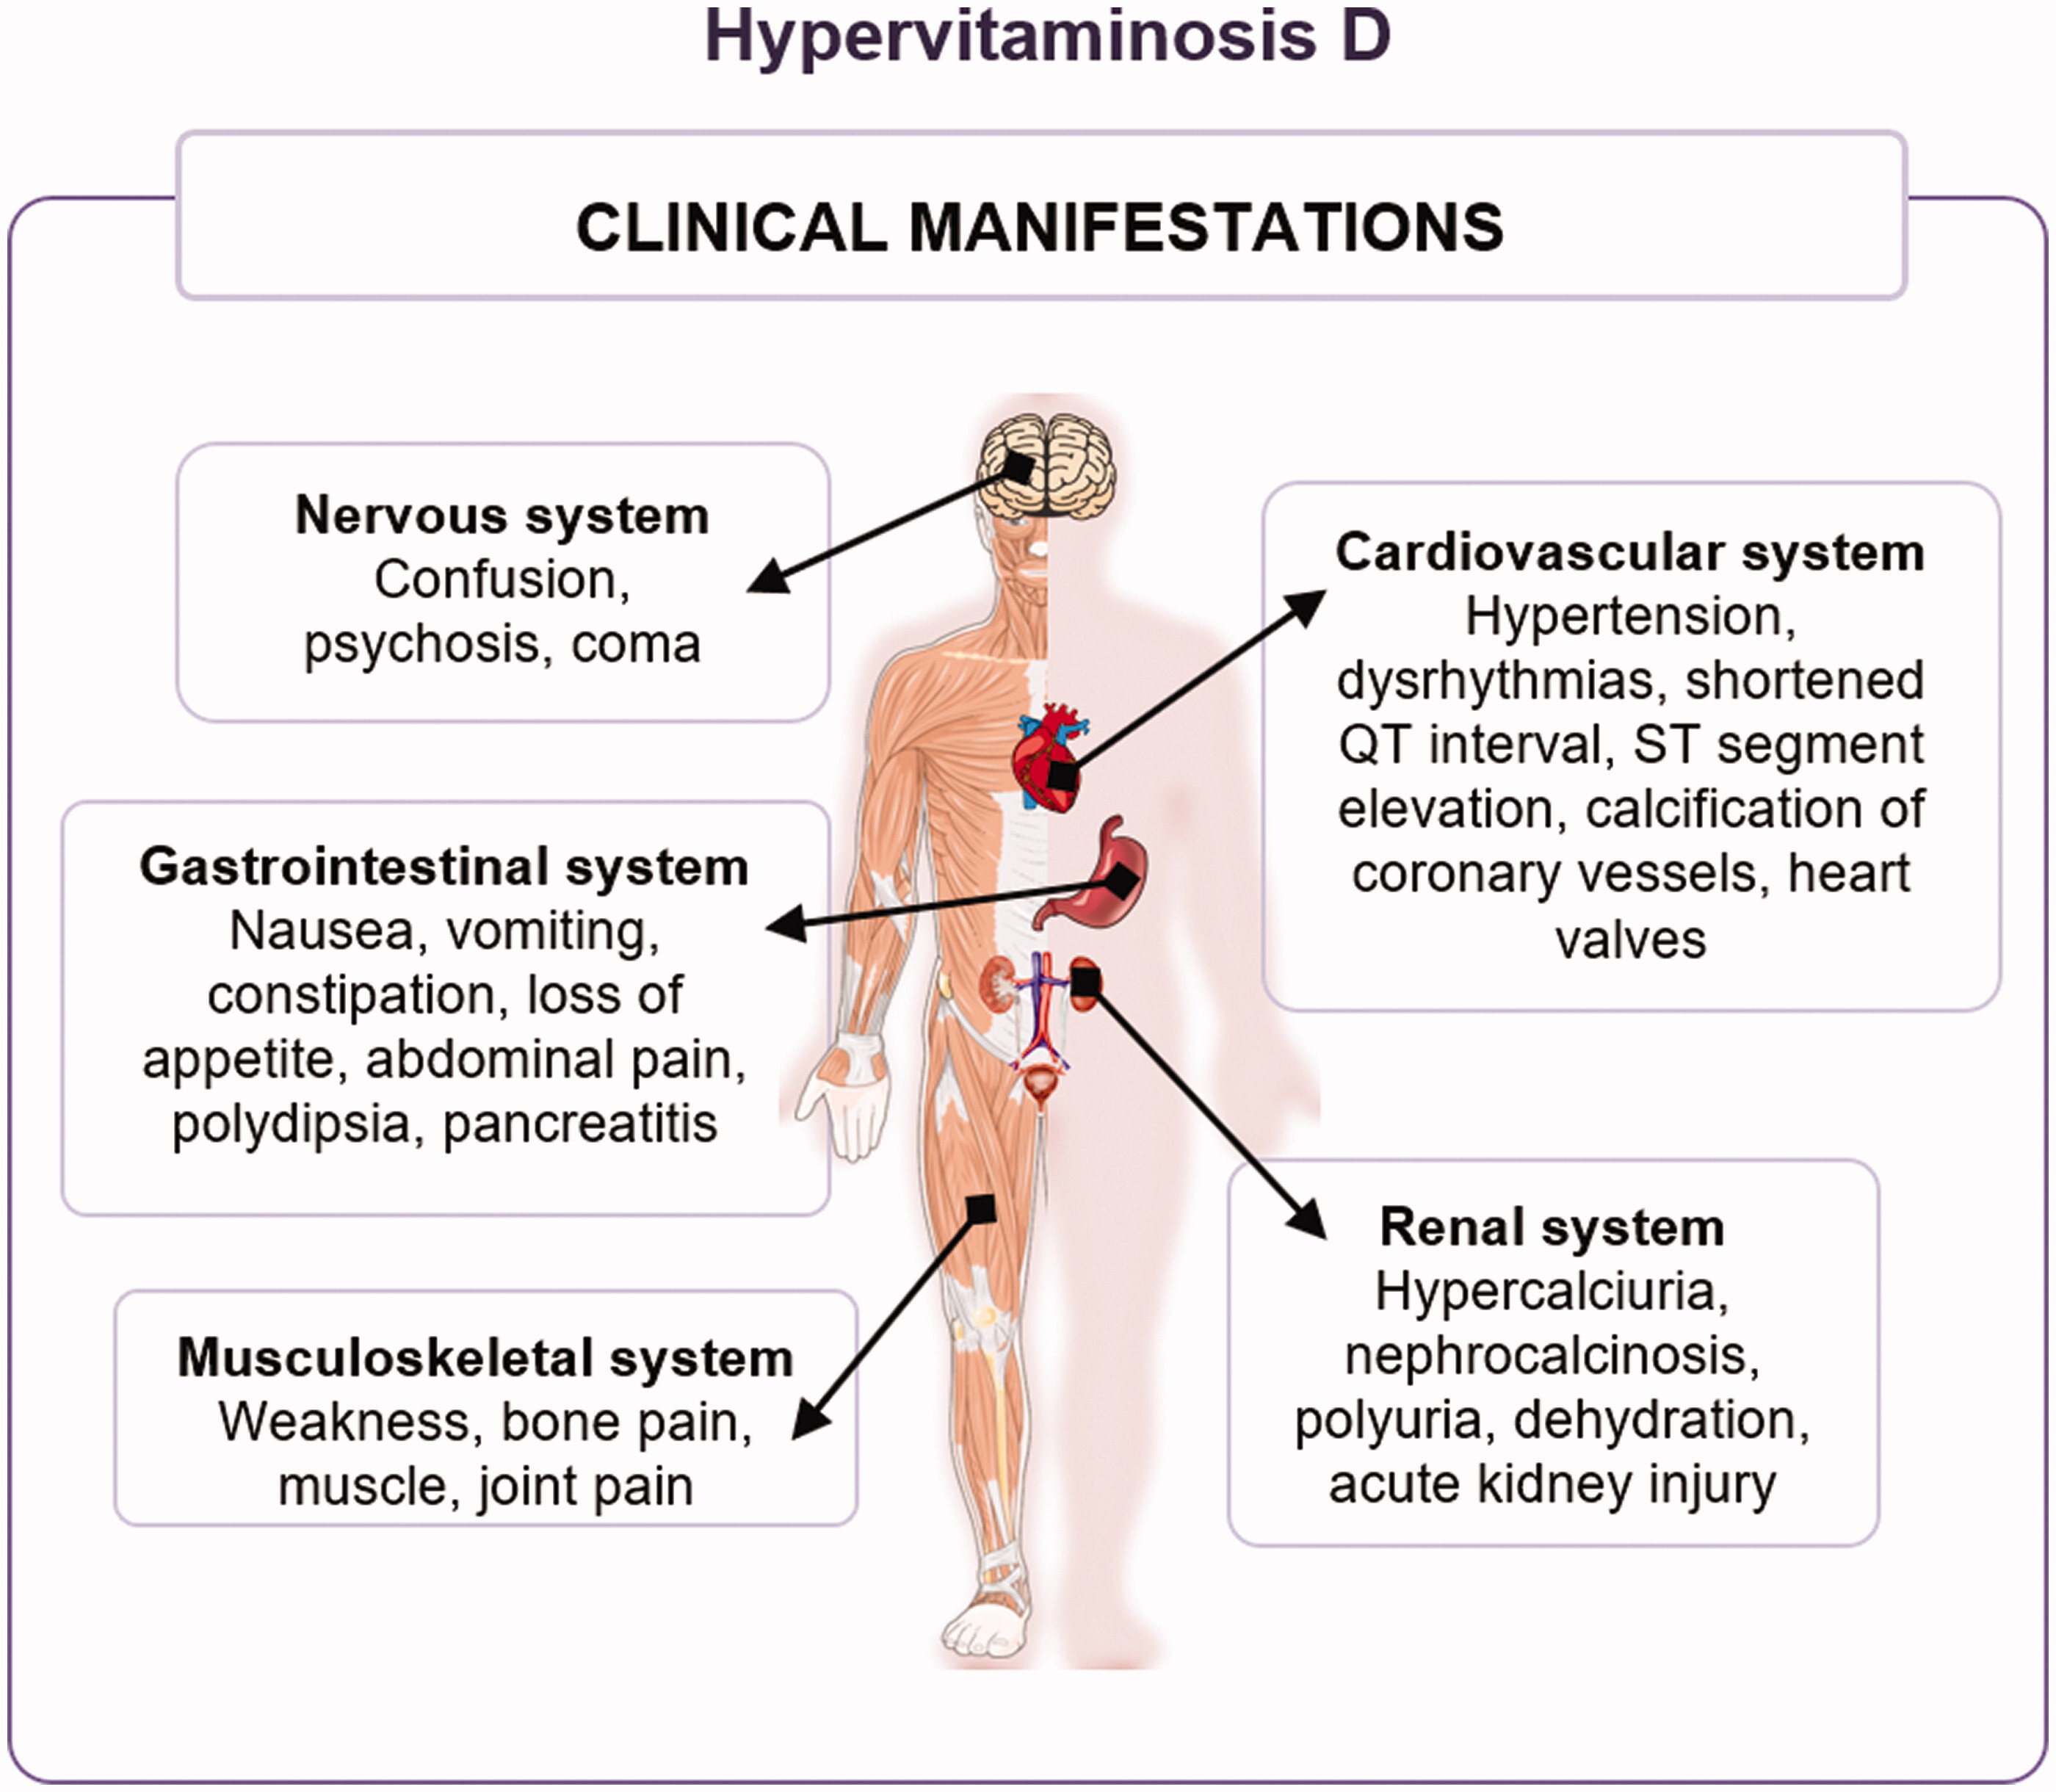
\includegraphics{figures/hypervitaminosis-d.jpg}

}

\caption[Symptômes associés lors d'une hypervitaminose
D.]{\label{fig-hypervitaminose-d}\textbf{Symptômes associés lors d'une
hypervitaminose D} \autocite{Janoušek.2022}.}

\end{figure}%

Le mécanisme de la toxicité due à la vitamine D n'est pas encore
totalement élucidé, mais il existe plusieurs hypothèses selon
\textcite{Jones.2008} s'appuyant sur le raisonnement lié à l'activation
du \ac{VDR} et de son action dans les cellules cibles
\autocite{Alshahrani.2013,Janoušek.2022}
(\textbf{Figure~\ref{fig-vd-intox-theory}}):

\begin{enumerate}
\def\labelenumi{\arabic{enumi}.}
\item
  La prise de vitamine D augmente les concentrations plasmatiques de
  calcitriol, ce qui augmente les concentrations cellulaires de
  calcitriol. L'étude de \textcite{DeLuca.2011} montre cependant que la
  toxicité de la vitamine D ne passe pas par le calcitriol. En effet,
  \textcite{DeLuca.2011} ont montré dans une expérience où des souris
  \ac{CYP27B1} KO constatent la même toxicité que le type sauvage
  possédant l'enzyme \ac{CYP27B1}. Les auteurs confirment ainsi que le
  calcitriol n'est pas le métabolite toxique dans leur étude.
  Similairement, les travaux de \textcite{Shepard.1980} montrent que le
  calcitriol diminue lorsque les doses de cholécalciférol sont trop
  élevées, par le biais du rétrocontrôle exercé par le calcium et le
  phosphate plasmatique ainsi que la \ac{PTH}.
\item
  La prise de vitamine D augmente les concentrations plasmatiques de
  calcidiol mol/L qui dépassent la capacité de liaison de la \ac{DBP} et
  le calcidiol libre pénètre dans la cellule, où elle aurait des effets
  directs sur l'expression des gènes. Lors d'une hypervitaminose D, les
  métabolites de la vitamine D saturent le \ac{DBP} dans le sang et la
  part de concentration libre du calcidiol augmente significativement
  \autocite{Jones.2008}. \textcite{DeLuca.2011} supportent l'idée que de
  la toxicité d'une hypervitaminose D serait due au calcidiol. En effet,
  l'étude de \textcite{Shepard.1980} montre que lorsque les doses
  d'administration de vitamine D augmentent chez le rat, augmentent la
  concentration en calcidiol tandis que la concentration en calcitriol
  décroît inversement avec la dose administrée. La concentration en
  calcidiol semble ne pas être régulée contrairement au calcitriol et
  pourrait être responsable de la toxicité due à une hypervitaminose D
  \autocite{DeLuca.2011,Shepard.1980}.
\item
  La prise de vitamine D augmente les concentrations de nombreux
  métabolites de la vitamine D, dont la vitamine D elle-même et le
  calcidiol. Ces concentrations dépassent la capacité de liaison de la
  DBP et provoquent la libération du calcitriol libre, qui pénètre dans
  les cellules cibles. L'étude de \textcite{Pettifor.1995} ayant pour
  but de déterminer le niveau de calcitriol lors d'une hypervitaminose
  D, montre que malgré le niveau de calcitriol bas observé, la
  concentration de calcitriol libre sont anormalement élevés, et cela
  est également corrélé avec la concentration de calcidiol. Les auteurs
  suggèrent que le calcitriol est déplacé de la \ac{DBP} par les
  concentrations micromolaires de calcidiol et d'autres métabolites non
  mesurés de la vitamine D tels que la 25-OHD-26,23 lactone, la
  24,25-(OH)\textsubscript{2}D et la 25,26(OH)\textsubscript{2}D.
  \textcite{Jones.2008} note que malgré les résultats de cette étude, il
  existe un manque de données additionnelles concernant cette hypothèse
  et que cette théorie reste non prouvée.
\end{enumerate}

\begin{figure}

\centering{

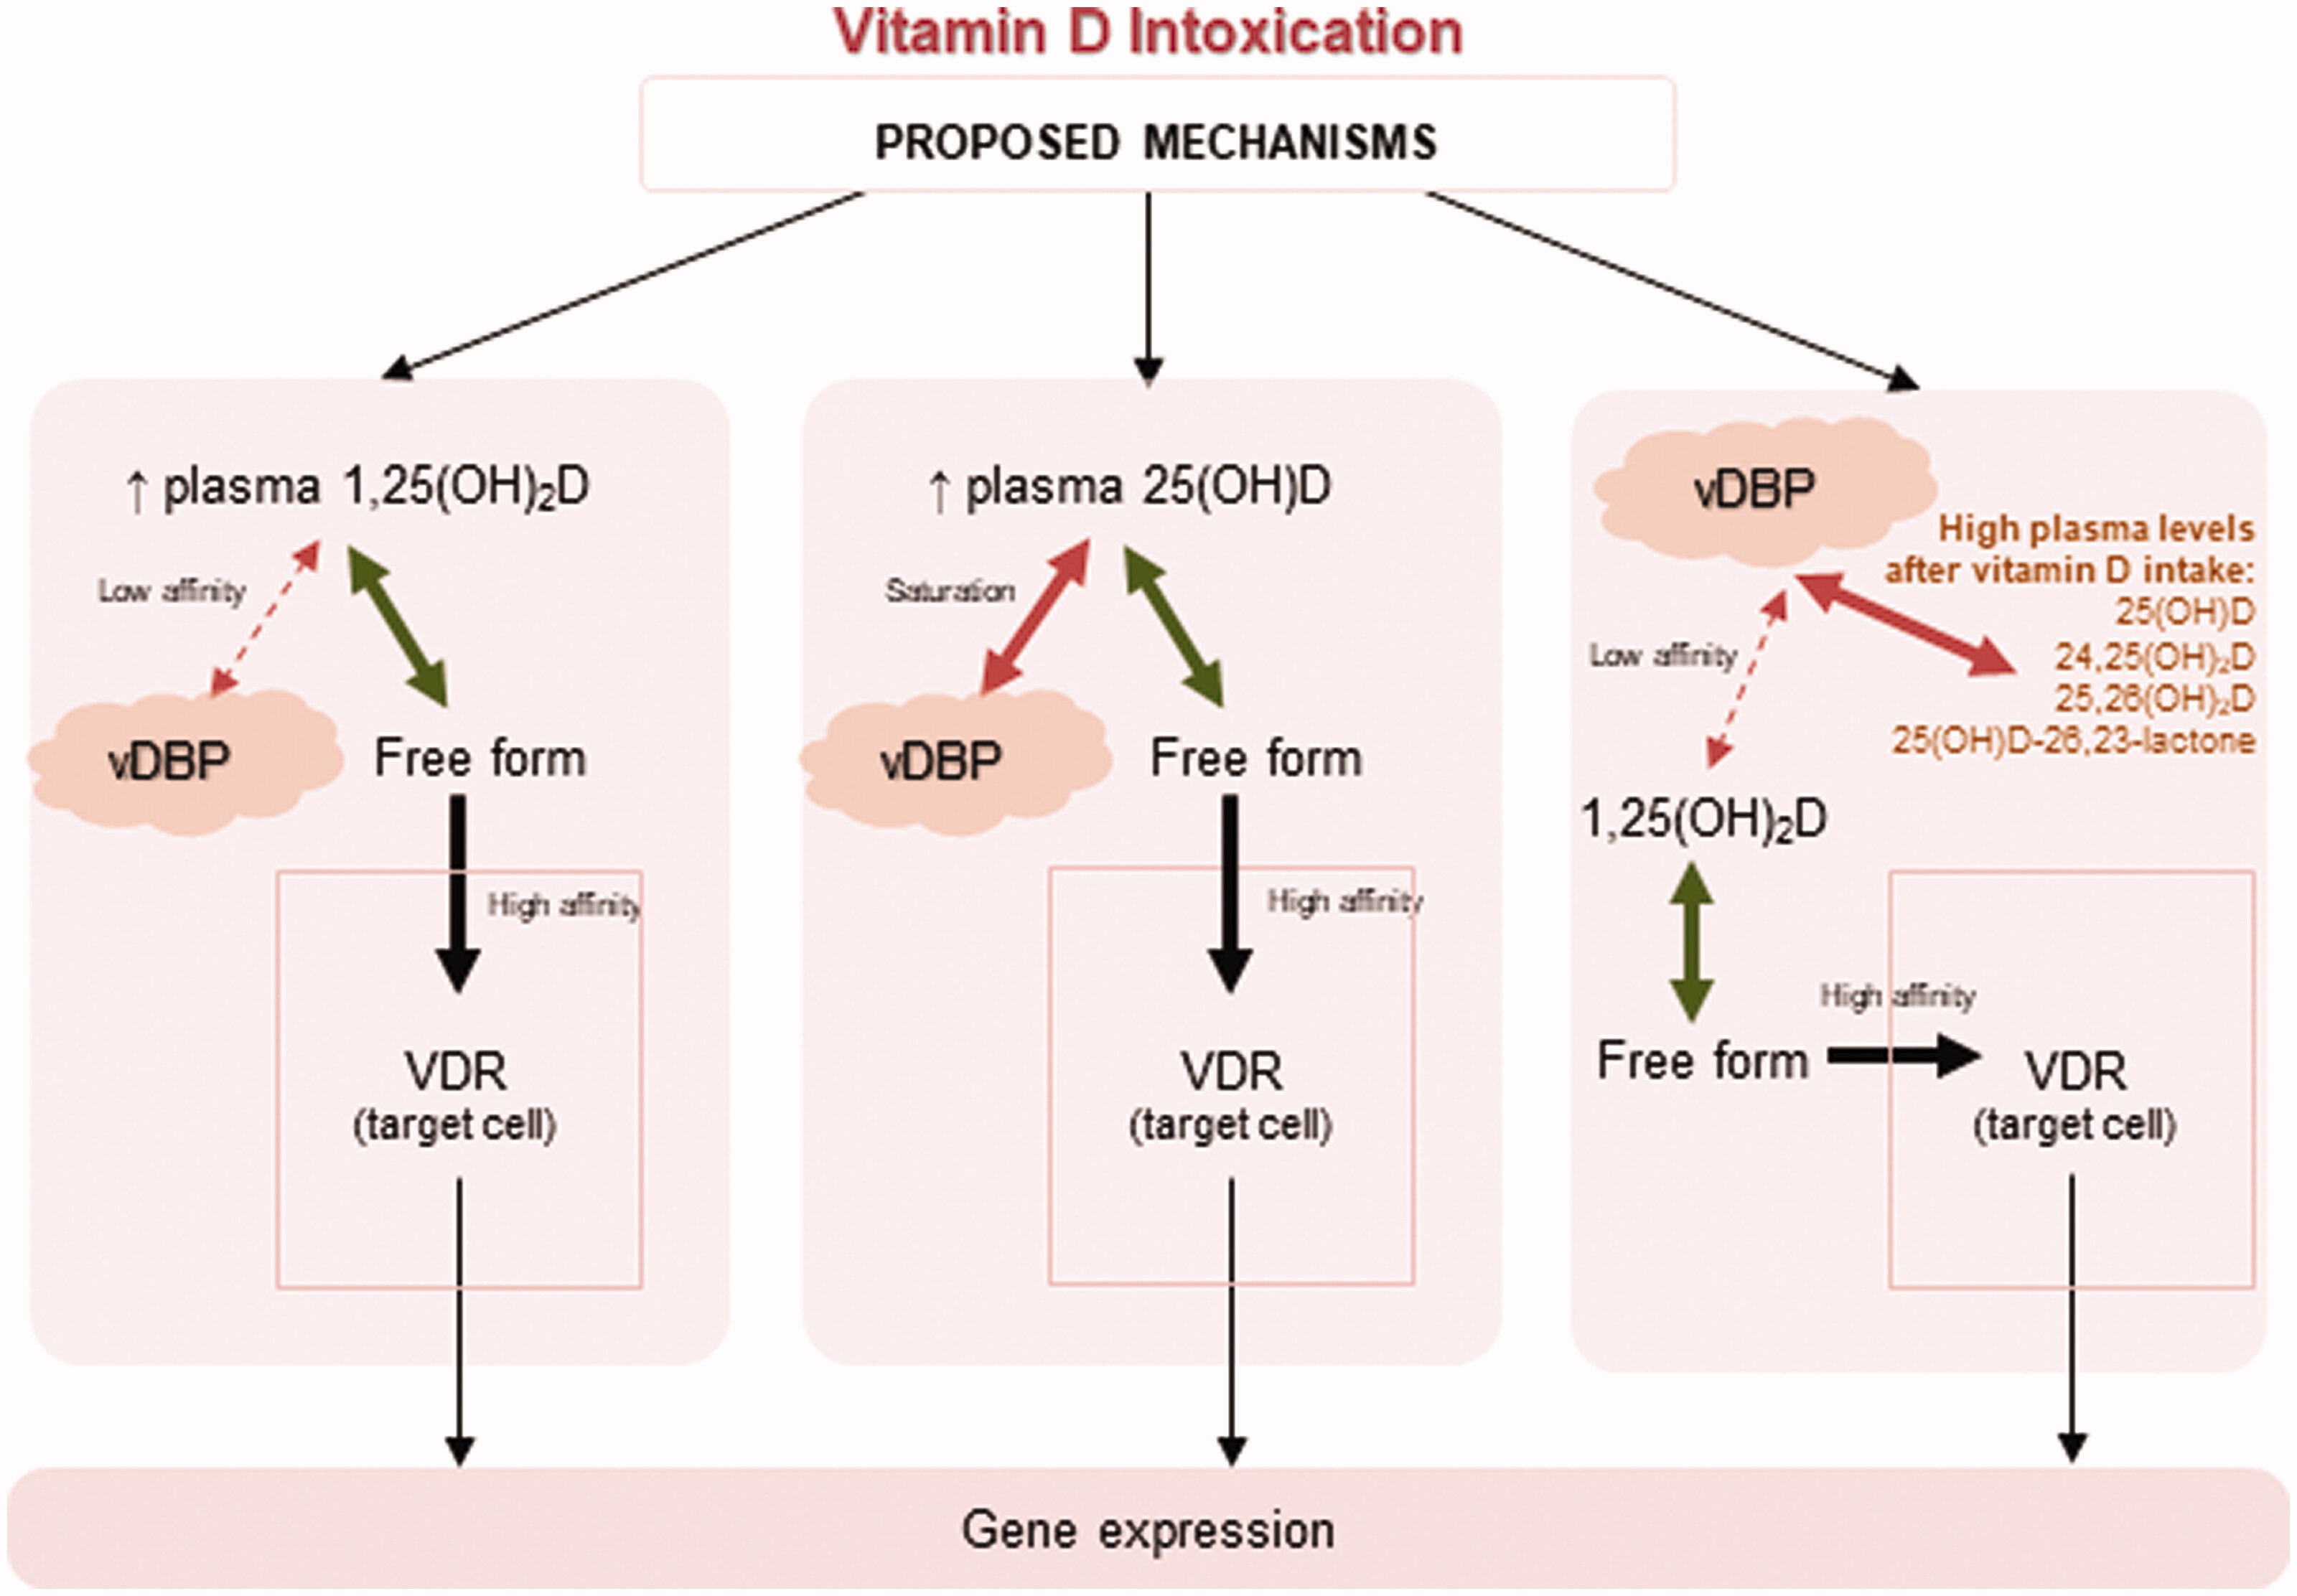
\includegraphics{figures/vd-intox-theory.jpg}

}

\caption[Trois théories proposées par \textcite{Jones.2008} pour
expliquer les mécanismes de toxicité de la vitamine
D.]{\label{fig-vd-intox-theory}\textbf{Trois théories proposées par
\textcite{Jones.2008} pour expliquer les mécanismes de toxicité de la
vitamine D} \autocite{Janoušek.2022}.}

\end{figure}%

Ainsi la toxicité de la vitamine D ne semble pas passer par le
calcitriol mais par une augmentation de calcidiol plasmatique. Lors
d'une hypervitaminose D, l'hypercalcémie issue de l'augmentation de
calcidiol plasmatique est due à une résorption osseuse accrue.
L'augmentation de calcium mène à une diminution de la production de
\ac{PTH}, et éventuellement, la diminution de la fonction rénale mène à
une réponse calciurique altérée ainsi qu'une perturbation de
l'homéostasie du calcium et du phosphate. Lorsque la fonction rénale
baisse par la suite, le processus d'absorption des tubules rénaux est
grandement perturbé ainsi que le débit de filtration glomérulaire.
L'hypercalcémie peut également conduire à une calcification des tissus
mous, et des vaisseaux sanguins. L'ensemble de ces conséquences
cardiovasculaires et rénaux causant une défaillance de ces systèmes est
probablement la cause d'une mort par intoxication de vitamine D. Il est
intéressant de noter que l'hypothèse selon laquelle un apport excessif
en vitamine D pourrait être associé à la formation de calculs rénaux
n'est pas appuyée par les données disponibles \autocite{IOM.2011}.

La toxicité de la vitamine D est habituellement due à une cause
iatrogène ou un excès de surdosage de vitamine D, pouvant être lié à un
accident, à des mauvaises pratiques médicales ou à un malentendu sur des
recommandations médicales \autocite{Lim.2020vd}. Elle peut aussi
survenir par une production endogène anormale de calcitriol chez les
patients à désordre granulomateux comme la sarcoïdose, la granulomatose,
les maladies fongiques, la léprose et bérylliose
\autocite{Marcinowska-Suchowierska.2018}.

La toxicité de la vitamine D est donc souvent due à un apport exogène,
puisque les apports endogènes ne permettent pas une concentration de
vitamine D aussi élevé. Cependant, il existe une toxicité endogène
rapportée dans la littérature à partir d'une production excessive de
25(OH)D et de 1,25(OH)\textsubscript{2}D dans des troubles congénitaux,
tels que le syndrome de Williams-Beuren, qui s'accompagne d'une
déficience en 24-hydroxylase, et donc ne permet pas la métabolisation de
25(OH)D\textsubscript{3} and 1,25(OH)\textsubscript{2}D\textsubscript{3}
en métabolites inactifs \autocite{Marcinowska-Suchowierska.2018}. Ce
syndrome cause ainsi une hypercalcémie, néphrolithiase, et
néphrocalcinose \autocite{Azer.2021}.

\subsection{Seuil de toxicité actuel}\label{seuil-de-toxicituxe9-actuel}

L'\ac{IOM} a déterminé la limite supérieure de sécurité (\ac{UL}) à 4000
UI/j de cholécalciférol. Ainsi, au-delà de cette limite, les auteurs
considèrent que le risque de toxicité augmente. Ce seuil a été déterminé
en partant du point d'observation où la prise de 10 000 UI/j de
cholécalciférol n'est pas associée à une toxicité classique pour des
adultes. Cette valeur est ensuite corrigée pour des raisons
d'incertitudes sur des données comme la mortalité toute causes,
concernant les prises inférieures à 10 000 UI/j, présentant des signes
de toxicité classiques pour des concentrations de calcidiol précédemment
considéré comme étant à la norme haute des valeurs physiologiques. Les
auteurs ont également considéré des différences ethniques potentielles.
La limite supérieure de sécurité des adultes concerne également les
enfants de 9 à 18 ans mais est réduite pour les enfants de 1 à 8 ans
(2500 à 3000 UI/j). Cependant l'\ac{IOM} admet que la toxicité de la
vitamine D est rare pour une valeur de 10 000 UI/j, mais que la toxicité
est plus commune vers des doses de 50 000 UI/j . Ces valeurs sont basées
sur des données limitées et que des études supplémentaires sont
nécessaires pour déterminer les effets de la vitamine D sur la santé
au-delà de ces valeurs \autocite{IOM.2011}.

L'\ac{ANSM} a publié un avis sur le bon usage de la vitamine D, suite à
des cas rapportés de surdosage de vitamine D entraînant une
hypercalcémie, parfois accompagnée de lithiase et néphrocalcinose chez
les enfants et nourrissons, après avoir pris une dose plus de deux fois
supérieure à la dose recommandée (400 UI par jour de 0 à 18 ans chez
l'enfant en bonne santé sans facteur de risque, 800 UI par jour de 0 à
18 ans chez l'enfant présentant un facteur de risque) pendant plusieurs
semaines, et deux cas d'intoxication sévère à la vitamine D après avoir
pris un complément alimentaire acheté sur internet contenant une dose de
10 000 UI par goutte. Il est notable de constater que ces cas
surviennent suite à une très grande dose de vitamine D par kg chez les
nourrissons et enfant, dont la dose devrait différer chez l'adulte
\autocite{ANSM.2021}.

\subsection{Questionnement sur le seuil de
toxicité}\label{questionnement-sur-le-seuil-de-toxicituxe9}

Le protocole Coimbra au Brésil utilise des doses de vitamine D nettement
supérieurs aux doses respectant les recommandations, pour traiter des
patients ayant des pathologies autoimmunes de la peau, telles que le
psoriasis ou vitiligo. \textcite{Amon.2022} ont effectué une étude sur
la sécurité du protocole pour répondre aux préoccupations autour du
risque d'hypercalcémie et de problèmes rénaux. Les patients prennent en
moyenne 35,291 ± 21,791 UI par jour, et peuvent même aller jusqu'à 300
000 UI par jour pour certaines pathologies. Pour la sclérose en plaque
le protocole recommande jusqu'à 1000 UI/kg/j, avec jusque là pas
d'effets indésirables avec plusieurs mois de traitements
\autocite{Lemke.2021}. Il existe un cas rapporté où un patient de 38 ans
était en hypercalcémie avec une concentration de 3,0 mmol/L, après 7
mois de traitement 100 000 UI de vitamine D par jour. Les auteurs
supposent que le patient possédait un gène causant des doses élevées de
\ac{PTH} et donc une hyperthyroïdie, ce qui serait la cause du cas
clinique observé. \textcite{Lemke.2021} concluent que les cas de
toxicité de vitamine D sont ainsi rares, mais que dans le cadre de leur
protocole, un dépistage d'une hyperthyroïdie et une surveillance
endocrinologique serait nécessaire.

Similairement, une étude clinique réalisée sur des patients atteints de
cancer utilise des doses de 10 000 UI de vitamine D\textsubscript{3}
sans observer d'effets indésirables \autocite{Amir.2010}. Les auteurs
notent une augmentation faible mais statistiquement significative du
calcium sérique a été observée, ainsi qu'une diminution significative de
la \ac{PTH} et qu'aucune modification significative des marqueurs de
résorption osseuse n'a été observée.

\textcite{Dudenkov.2015} ont conduit une étude pour déterminer la
tendance de l'incidence des valeurs de 25(OH)D supérieures à 50 ng/mL de
2002 à 2011 et leur association avec l'hypercalcémie. L'étude
rétrospective est conduite sur 20 308 patients dans une période de 10
ans de suivi. \textcite{Dudenkov.2015} partent des recommandations de
l'IOM définissant le seuil de limite supérieure de 4000 UI/j,
correspondant à un sérum de 50 ng/mL de calcidiol selon les auteurs. Les
valeurs sériques de 25(OH)D n'étaient pas significativement liées aux
valeurs de calcium sérique (\emph{P} = 0.20) ou au risque
d'hypercalcémie (\emph{P} = 0.24). Ils concluent que malgré que
l'incidence de patients ayant des valeurs de calcidiol supérieures à 50
ng/mL ait augmenté, l'incidence de cas de toxicité clinique aiguë de
vitamine D reste la même.

Puisque d'autres effets bénéfiques semblent apparaître lorsque la dose
de vitamine D est supérieure à la dose recommandée (600-800 UI/j),
l'équipe de \textcite{Hathcock.2007} a conduit une méta-analyse,
cherchant à identifier la \ac{NOAEL}, seuil pour laquelle aucun effet
indésirable n'est observé. Sur la base de deux études cliniques
robustes, les auteurs ont considéré qu'une dose de 10 000 UI par jour,
correspondant à 100 ng/mL serait adéquate pour définir la \ac{NOAEL},
associant une augmentation de la vitamine D sans pour autant observer un
changement anormal de la calcémie. Aucun effet indésirable n'a été
observé dans les essais cliniques utilisant une dose inférieure à ce
seuil. Les auteurs notent que les cas de toxicité rapportés à la
vitamine D surviennent pour des concentrations de vitamine D, allant à
des doses supérieures à 280 ng/mL jusqu'à 640 ng/mL. De plus, les
auteurs ont identifié une \ac{LOAEL}, seuil pour laquelle des effets
indésirables sont observés, sur la base d'une étude nécessitant 77 000
UI/j, ce qui correspond à 240 ng/mL, une dose entraînant
l'hypercalcémie. Les auteurs notent également que les patients utilisés
dans l'étude ont une sensibilité accrue à la vitamine D, et donc que le
seuil identifié est donc conservatif, et augmente l'assurance du seuil
\ac{NOAEL} et \ac{LOAEL}.

J'ai obtenu les informations suivantes sur la base d'un article écrit
par \textcite{Holick.2015} : \textgreater{} \emph{Les origines de la
dose si basse en vitamine D viennent d'une succession d'évènement
débutant vers la fin du 19\textsuperscript{ème} début
20\textsuperscript{ème}. Ainsi, plus de 80\% des enfants possédaient des
déformations associées au rachitisme ainsi qu'un retard de la croissance
osseuse et des difformités osseuses en Europe et sur la côte Est des
Etats-Unis. En 1921, Hess et Unger rapportent que l'exposition au soleil
guérissent les enfants du rachitisme, ce qui a entraîné la fortification
du lait en vitamine D2 (produite à partir de l'ergostérol végétal) et
d'autres aliments tels que du pain, des boissons gazeuses, de la bière,
de la crème anglaise et même des hot-dogs. Vers les années 1950s,
plusieurs cas ont été signalé en Angleterre de nourrissons présentant
des anomalies faciales accompagnées d'hypercalcémie et de sténose
aortique supra-valvulaire. Les médecins concluent indirectement en se
basant sur la littérature et les données cliniques disponibles qu'il
s'agit d'une intoxication à la vitamine D. Cela a engendré un mouvement
contraire où les recommandations sur les doses de vitamine D ont été
établies conservativement afin d'éviter l'hypercalcémie chez les
nourrissons, ainsi que l'interdiction dans de nombreux pays de fortifier
le lait avec de la vitamine D. Cependant, avec rétrospection, la
littérature suggère que les nourrissons alors rapportés avaient le
syndrome de Williams-Beuren, et donc étaient hypersensible à la vitamine
D et présentaient les symptômes rapportés. Il ne s'agissait donc pas
d'une situation clinique normale liée à la toxicité vitamine D mais à
l'hypersensibilité à la vitamine D \autocite{Holick.2015}.}

\newpage{}

\chapter{Vitamine D, système immunitaire et réponse
antivirale}\label{vitamine-d-systuxe8me-immunitaire-et-ruxe9ponse-antivirale}

L'importance cruciale du rôle de la vitamine D sur le système
immunitaire a récemment captivé l'attention des chercheurs depuis la
découverte de la coexistence du \ac{VDR} et du \ac{CYP27B1} dans des
tissus dont la fonction n'est pas directement liée à l'homéostasie du
calcium \autocite{Zehnder.2001}. En particulier, l'expression du
\ac{CYP27B1} dans les cellules immunitaires est régulée indépendamment
de l'homéostasie du calcium, en présence ou non de pathogènes, ce qui
démontre le rôle central de la vitamine D dans la régulation du système
immunitaire \autocite{White.2022}.

La vitamine D agit à la fois sur les cellules du système immunitaire
inné et adaptatif par de nombreuses fonctions et effets
(\Cref{tbl:vd-immu}). Deux observations principales supportent la
théorie du rôle de la vitamine D dans le système immunitaire : le
récepteur au calcitriol est présent dans toutes les cellules
immunitaires, et la présence de l'enzyme de conversion finale du
calcidiol en calcitriol, la 1α-hydroxylase est uprégulée par certaines
cellules immunes \autocite{Giannini.2022}.

Ainsi, plusieurs cellules immunitaires peuvent synthétiser l'enzyme clé
permettant la conversion du 25(OH)\textsubscript{2}D\textsubscript{3} en
1,25(OH)\textsubscript{2}D\textsubscript{3}, le cytochrome CYP27B1 ou
aussi appelée 1α-hydroxylase. L'induction de cette enzyme concerne des
cellules telles que les cellules dendritiques, monocytes, macrophages,
lymphocytes B et T \autocites[ ]{Giannini.2022}{Dankers.2017}.

Dans ce contexte, l'enzyme 1α-hydroxylase n'est pas uprégulée par la
\ac{PTH}. Par conséquent, la production de
1,25(OH)\textsubscript{2}D\textsubscript{3} dépend des niveaux de
substrat de 25(OH)D\textsubscript{3} et peut être régulée par des
signaux inflammatoires, tels que le \ac{LPS} et les cytokines
\autocite{Giannini.2022}.

\begin{table}
\centering
\caption[Effets de la vitamine D sur le système immunitaire.]{\textbf{Effets de la vitamine D sur le système immunitaire.} Le tableau montre les effets de la vitamine D sur le système immunitaire inné et adaptatif. Globalement, la vitamine D possède un effet immunomodulateur. D'après \textcite{Giannini.2022}.}
\label{tbl:vd-immu}
\begin{tabular}{lc}
\toprule
\textbf{Fonction/Cellules} & \textbf{Effet} \\
\midrule
\textbf{Immunité Innée} & \\
Différenciation des macrophages & Augmentation \\
Elimination des bactéries & Augmentation \\
Maturation des cellules dendritiques & Diminution \\
Présentation antigénique & Diminution \\
\midrule
\textbf{Immunité adaptative} & \\
Cytokines Th$_1$ & Diminution \\
Cytokines Th$_2$ & Augmentation \\
Différentiation des Th${_{17}}$ & Diminution \\
Différentiation des T\textsubscript{reg} & Augmentation \\
\addlinespace
\multirow{4}{*}{Lymphocytes B} & Diminution de la prolifération \\
& Induction de l'apoptose \\
& Inhibition de la génération des plasmocytes \\
& Inhibition de la sécrétion des immunoglobulines\\
\bottomrule
\end{tabular}
\end{table}

\section{Schéma d'une réponse antivirale
classique}\label{schuxe9ma-dune-ruxe9ponse-antivirale-classique}

La voie des interférons de type I (IFN-1) est centrale dans la réponse
antivirale initiale. Elle permet d'inhiber la réplication virale, de
protéger les cellules non-infectées et de stimuler l'immunité
lymphocytaire antivirale (lymphocytes T CD8, NK). Ces mécanismes
d'immunité innée conduisent à la lyse des cellules infectées et à
l'instauration d'une immunité durable. Dans l'ensemble, ces processus
éliminent le virus, limitent l'atteinte pulmonaire et mènent à une
potentielle guérison.

\section{Mécanismes d'action de la vitamine D sur le système
immunitaire}\label{muxe9canismes-daction-de-la-vitamine-d-sur-le-systuxe8me-immunitaire}

La vitamine D possède une action globalement anti-inflammatoire et donc
régulatrice de l'inflammation (\Cref{fig-vd-immune-effect}). Elle agit à
la fois sur le système immunitaire inné et adaptatif. A l'initiation de
la réponse inflammatoire, le calcitriol est essentiel afin de répondre à
une infection. Les effets de la vitamine D ne répriment pas totalement
le système immunitaire mais plutôt induit une modulation immunitaire, en
faisant évoluer le système immunitaire adaptatif vers une tolérance
antigénique, et le système immunitaire inné vers une meilleure
élimination virale et bactérienne \autocite{Martens.2020}. Le calcitriol
n'est donc pas purement anti-inflammatoire mais il contribue à maintenir
l'équilibre entre un état pro- et anti-inflammatoire et est donc capable
de rétablir l'équilibre perturbé \autocite{Dankers.2017}.

\begin{figure}

\centering{

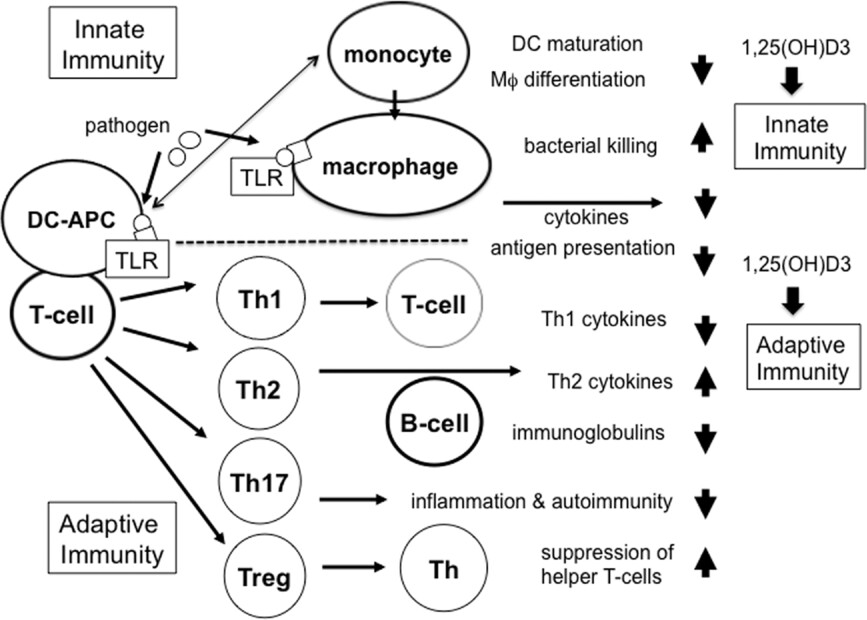
\includegraphics{figures/vd-immune-effect.jpg}

}

\caption[Effets du calcitriol sur les réponses immunitaires sous des
conditions normales.]{\label{fig-vd-immune-effect}\textbf{Effets du
calcitriol sur les réponses immunitaires sous des conditions normales.}
La 1,25(OH)\textsubscript{2}D\textsubscript{3} régule à la fois
l'immunité innée et l'immunité adaptative, en potentialisant la réponse
innée (activité antimicrobienne des macrophages), en diminuant la
présentation de l'antigène et en supprimant l'immunité adaptative
(fonctions des lymphocytes B et de certains lymphocytes T). Cependant,
dans des conditions normales, la
1,25(OH)\textsubscript{2}D\textsubscript{3} augmente les cytokines T
helper (Th\textsubscript{2}) (c'est-à-dire l'interleukine 10) et
l'efficacité des T\textsubscript{reg}. DC, cellules dendritiques ; APC,
cellules présentatrices d'antigènes ; TLR, Toll-like receptor ;
T\textsubscript{reg}, lymphocytes T régulateurs. D'après
\textcite{Cutolo.2014}}

\end{figure}%

\subsection{Effets de la vitamine D sur les cellules immunitaires
innées}\label{effets-de-la-vitamine-d-sur-les-cellules-immunitaires-innuxe9es}

Plusieurs signaux sont nécessaires à l'induction de la 1α-hydroxylase,
tels que la présence d'activateurs de macrophages et de monocytes comme
le \ac{tnfa} ou l'\ac{ifng}, ainsi que les récepteurs innés \acp{TLR}.
Lorsque les cellules sont activées, elles expriment le \ac{CYP27B1} qui
va permettre de métaboliser le calcidiol en calcitriol
\autocite{Liu.2006,Charoenngam.2020}.

\subsubsection{Macrophages et monocytes}\label{macrophages-et-monocytes}

Le calcitriol peut ensuite agir de manière intracrine via un signalement
médié par l'hétérodimère \ac{VDR}-\acsu{RXR} (\acl{RXR}), causant
l'importation de cet hétérodimère dans le noyau va induire la production
de cathélicidine LL-37 et de β2-défensine (Figure~\ref{fig-vd-action})
\autocite{Caprio.2017,Yasmin.2005}. La cathélicidine est un peptide
antimicrobien luttant contre les bactéries et les fongi en déstabilisant
leurs membranes \autocite{Charoenngam.2020}. Le calcitriol est capable
entre autres d'induire la reconnaissance des pathogènes par le biais du
\ac{TLR} et le switch phénotypique de macrophage M1 vers M2 par la
régulation positive de l'\ac{IL-10}. Le macrophage M2 est un type de
macrophage ayant un profil anti-inflammatoire contrairement au
macrophage M1 au profil pro-inflammatoire. Le calcitriol inhibe
également des cytokines majeures pro-inflammatoires telles que
l'\ac{IL-6} et le \ac{tnfa} \autocite{Meza-Meza.2022,Caprio.2017}. Il a
également été démontré que le calcitriol supprime l'expression des
\ac{TLR} sur les monocytes et inhibe la production des cytokines
inflammatoires \ac{IL-2}, l'\ac{IL-6} et l'\ac{IL-17}. La vitamine D
stimule également le signalement cytokinique, avec induction de
chimiokines comme l'IL-8/CXCL8, une chimiokine agissant sur le
neutrophile.

Le calcitriol libéré joue également un rôle paracrine, puisqu'il sort de
la cellule et va ensuite influencer les diverses cellules immunitaires
environnantes (Figure~\ref{fig-vd-action}). Il est intéressant de noter
une conséquence involontaire de cette fonction paracrine est que les
macrophages peuvent produire une quantité excessive de calcitriol qui
pénètre dans la circulation et stimule de manière non régulée
l'absorption intestinale du calcium et la mobilisation du calcium
osseux, ce qui entraîne une hypercalciurie et une hypercalcémie dans des
conditions pathologiques inflammatoires telles que des désordres
granulomateux et les lymphomes \autocite{Charoenngam.2020}.

\begin{figure}

\centering{

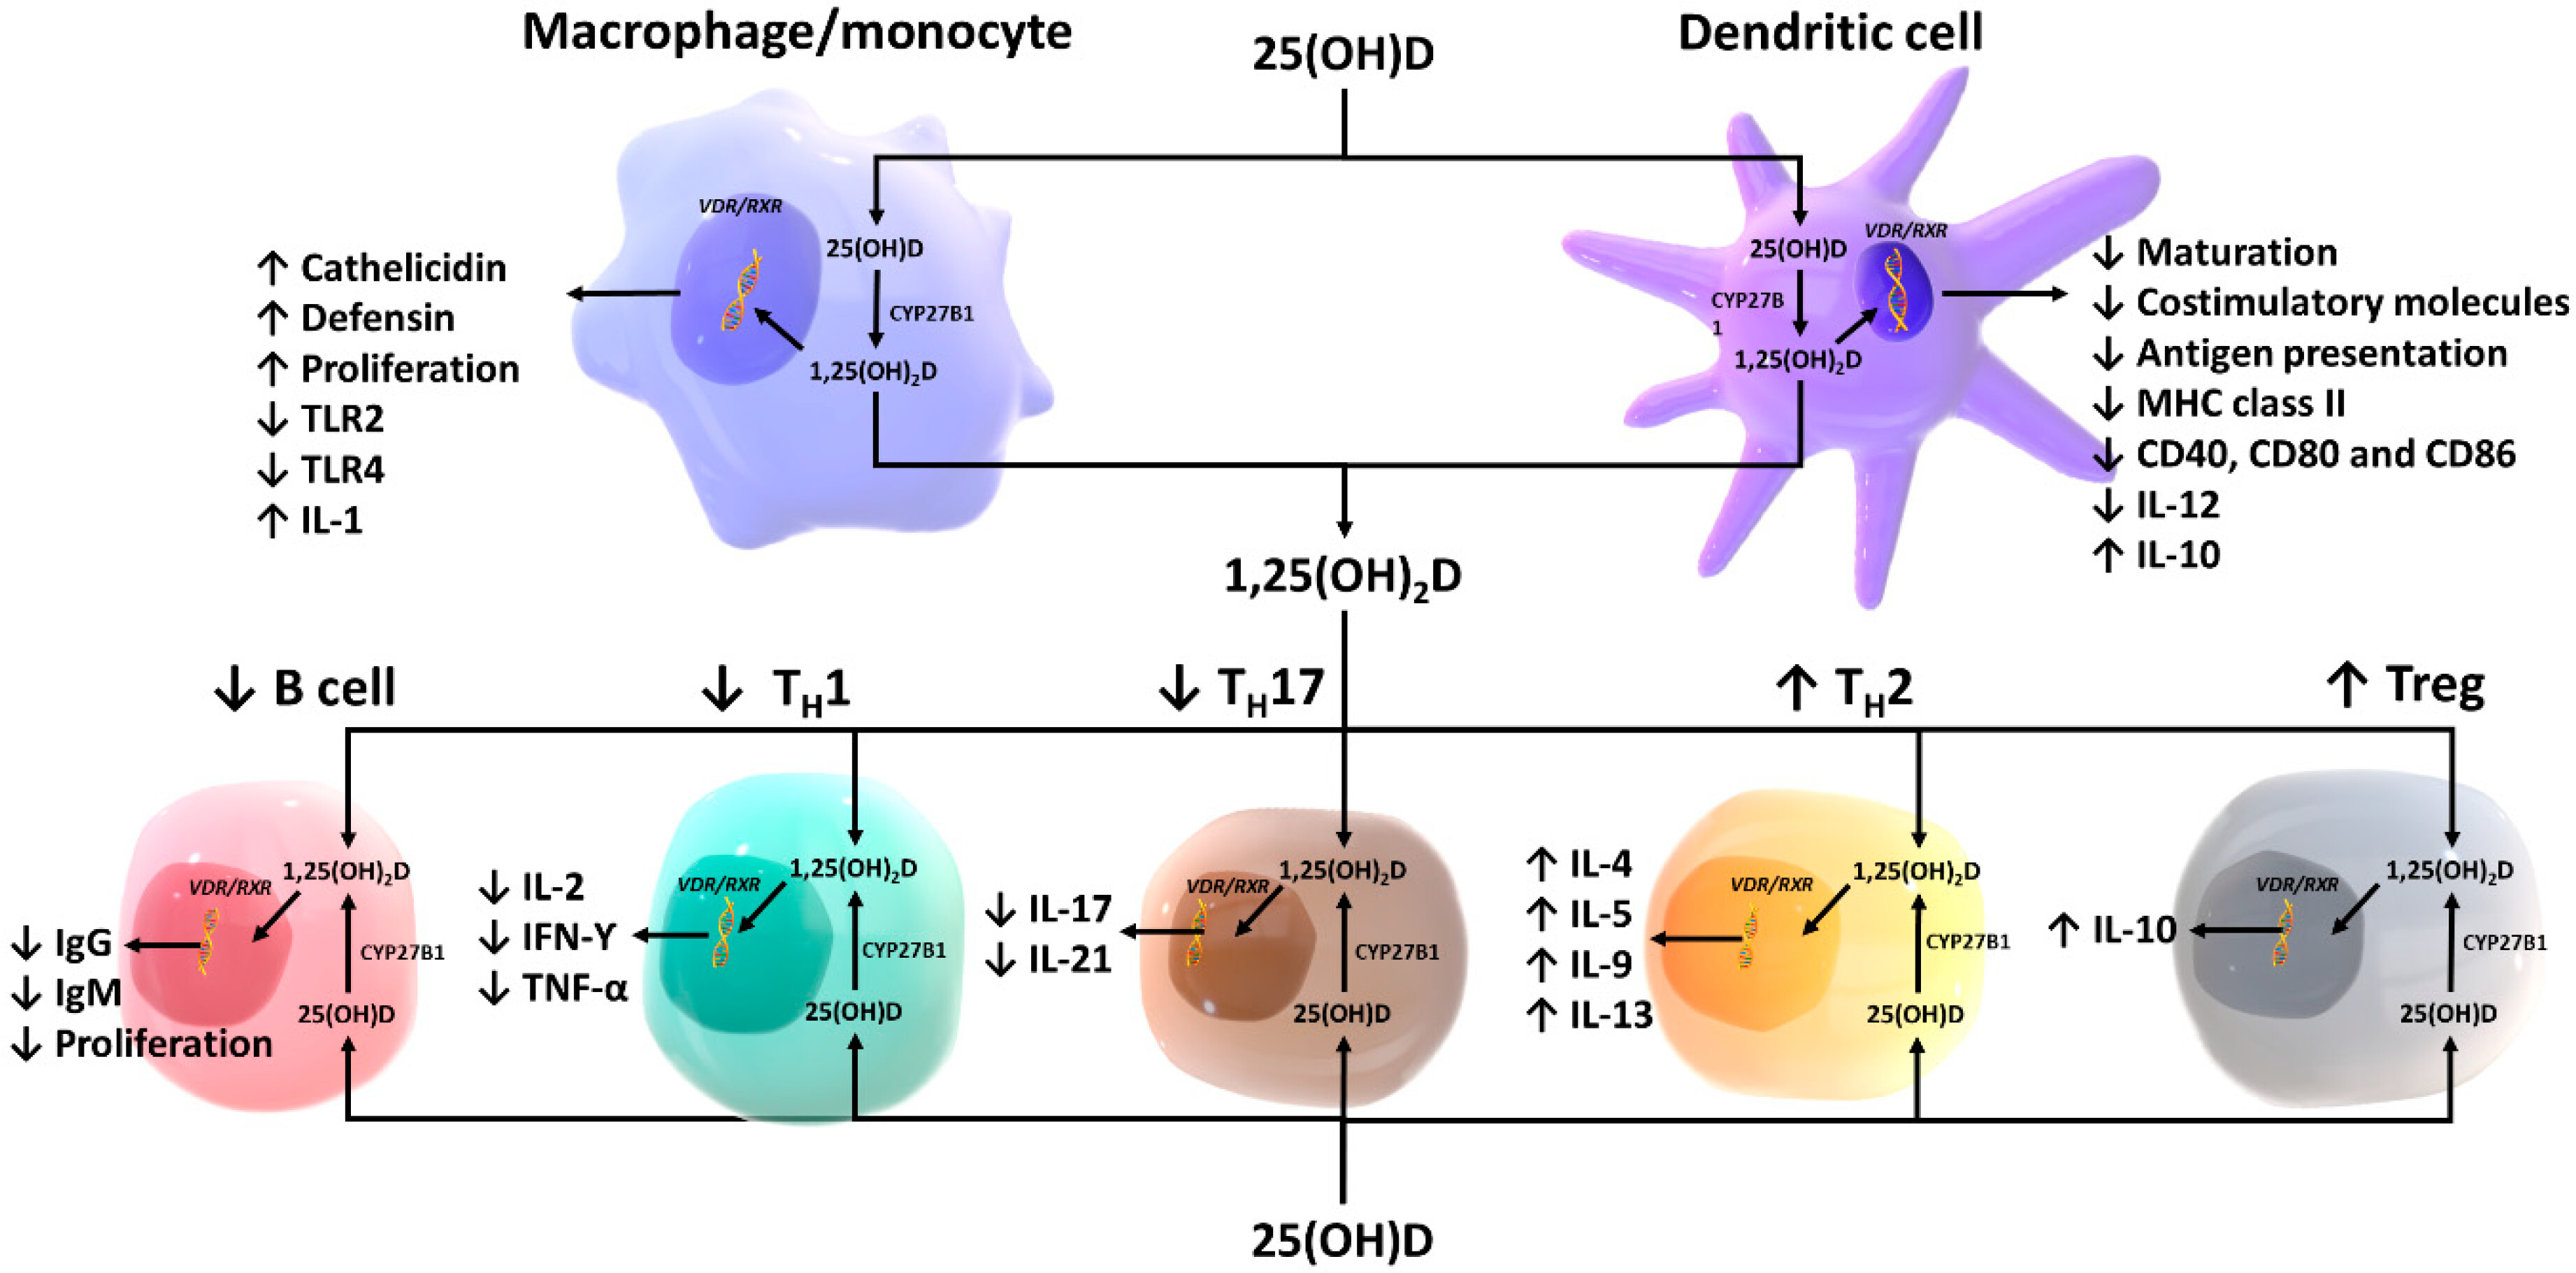
\includegraphics{figures/vd-action.jpg}

}

\caption[Représentation schématique des fonctions paracrine et
intracrine de la vitamine D et de ses métabolites et des actions de la
1,25-dihydroxyvitamine D sur les systèmes immunitaires innés et
adaptatifs.]{\label{fig-vd-action}\textbf{Représentation schématique des
fonctions paracrine et intracrine de la vitamine D et de ses métabolites
et des actions de la 1,25-dihydroxyvitamine D sur les systèmes
immunitaires innés et adaptatifs.} Les macrophages, monocytes et
cellules dendritiques sont capables d'induire le \ac{CYP27B1} afin de
métaboliser le calcidiol en calcitriol, qui va ensuite agir de manière
intracrine par le biais de la translocation de l'hétérodimère
\ac{VDR}-\ac{RXR} et agir directement sur l'expression des facteurs de
transcription. Globalement les effets issus du calcitriol seront liés à
l'augmentation de la défense antimicrobienne notamment par le biais de
la cathélicidine, ainsi qu'une diminution du phénotype mature de la
cellule dendritique et une augmentation du phénotpe tolérogène. Par la
suite, le calcitriol peut agir sur les cellules environnantes en
favorisant un phénotype anti-inflammatoire chez les cellules
T\textsubscript{h2} et T\textsubscript{reg} ainsi qu'une diminution de
l'activation des cellules T\textsubscript{h1} et T\textsubscript{h17},
et des cellules B. Abréviation : 1,25(OH)2D : 1,25-dihydroxyvitamine D ;
25(OH)D : 25-hydroxyvitamine D ; IFN-Ƴ : interféron- Ƴ ; IL :
interleukine ; CMH : complexe d'histocompatibilité membranaire ; RXR :
Nuclear Receptor Retinoid X Receptor ; TH1 : T helper 1 ; TH2 : T helper
2 ; TH17 : T helper 17 ; Treg : cellule T régulatrice ; TNF-α : Tumor
necrosis factor- α ; TLR2 : toll-like receptor 2 ; TLR4 : toll-like
receptor 4; VDR : Vitamin D Receptor. \autocite{Charoenngam.2020}}

\end{figure}%

\subsubsection{Cellules présentatrices d'antigènes et lymphocytes
NK}\label{cellules-pruxe9sentatrices-dantiguxe8nes-et-lymphocytes-nk}

Le calcitriol agit également sur les \ac{CPA}, concernant notamment les
cellules dendritiques, macrophages et lymphocytes B, et les \ac{NK} en
les rendant plus immature et tolérogéniques, par le biais d'une
diminution de l'expression de \ac{CMH-II} qui leur permet de présenter
des antigènes étrangers, ainsi que l'expression de molécules de
co-stimulation (\ac{CD} 40, CD80, CD86) qui jouent un rôle essentiel
dans la stimulation des lymphocytes (Figure~\ref{fig-vd-action})
\autocite{Charoenngam.2020,Meza-Meza.2022,Caprio.2017}. Ce changement
phénotypique s'accompagne donc d'une diminution de la capacité de
présentation d'antigènes et de production d'\ac{IL-12}, interleukine clé
pour la différenciation des lymphocytes T en Th1, l'activité cytotoxique
des lymphocytes \ac{NK} et lymphocytes CD8\textsuperscript{+}, ainsi
qu'une augmentation d'\ac{IL-10}, une cytokine clé dans la régulation du
système immunitaire.

En outre, des études expérimentales ont suggéré que la différenciation
et la fonction des lymphocytes \ac{NK} peuvent être modulées par un
traitement au calcitriol \autocite{Charoenngam.2020}. Cependant, le rôle
inducteur ou inhibiteur du calcitriol est encore indéterminé par manque
de données cohérentes.

\subsubsection{Fonction endothéliale et perméabilité
vasculaire}\label{fonction-endothuxe9liale-et-permuxe9abilituxe9-vasculaire}

De nombreuses études expérimentales ont démontré que la vitamine D et
ses métabolites ont la capacité de moduler la fonction endothéliale et
la perméabilité vasculaire par le biais de diverses voies génomiques et
non génomiques. Il a été démontré que la vitamine D\textsubscript{3}, le
calcidiol et le calcitriol stabilisent l'endothélium vasculaire de
manière non génomique, le cholécalciférol étant plus puissante que le
calcidiol et calcitriol à cet égard. En outre, le calcitriol agit comme
un régulateur transcriptionnel de l'oxyde nitrique synthase endothéliale
(\acs{eNOS})\acused{eNOS}, favorisant l'uprégulation de l'expression
génétique de l'\ac{eNOS} et augmentant la production d'\ac{NO} par les
cellules endothéliales. L'apparition rapide en une minute de l'effet du
calcitriol suggère un mécanisme d'action non génomique, soit une action
ne passant pas par une transcription de gènes. L'activation du \ac{VDR}
au niveau de la membrane des cellules endothéliales déclenche des voies
intracellulaires telles que les voies AC/cAMP, IP3 /DAG et PI3K/Akt, ce
qui entraîne une augmentation de la concentration de calcium
intracellulaire et l'activation de la \ac{eNOS}. En outre, des études
ont montré que le calcitriol favorise la formation de jonctions
cellule-cellule et inhibe l'organisation des fibres de stress dans
l'endothélium \autocite{Charoenngam.2020}.

Le calcitriol possède d'autres effets au regard de l'épithélium
intestinal et des cellules de Paneth en augmentant la viabilité des
cellules épithéliales intestinales et atténue les dommages causés à
l'épithélium intestinal par le \ac{LPS} bactérien. La vitamine D est
également capable d'agir non-classiquement par des actions
non-génomique, c'est-à-dire que l'effet de la liaison du calcitriol sur
le VDR ne nécessite pas nécessairement sa translocation dans le noyau
pour avoir des effets et donc l'usage du \ac{VDRE}, mais peut agir
directement par des actions de type protéine-protéine. Cela permet à la
vitamine D de moduler des voies dont les ligands n'interagissent pas
avec la vitamine D, telle que l'inhibition de la kinase \ac{IKKb}, un
régulateur de la voie canonique de \ac{nfkb} passant par le ligand
\ac{tnfa}, une des cytokines pro-inflammatoire clé de la réaction
immunitaire, ou l'interaction avec STAT1 qui permet de moduler cette
voie dont le ligand est l'\ac{ifna}, par la transcription de gène
anti-viraux. Ce mécanisme non-génomique permet à la vitamine D de
moduler entre autre des réponses immunes anti-virales \autocites[
]{Hii.2016}{Chen.2013.IKKb}.

\subsection{Effets de la vitamine D sur l'immunité
adaptative}\label{effets-de-la-vitamine-d-sur-limmunituxe9-adaptative}

La vitamine D joue un rôle essentiel dans la modulation des réponses
immunitaires adaptatives, en particulier des lymphocytes T et B, qui
sont les principales cellules immunitaires de cette composante du
système immunitaire. Les lymphocytes T sont responsables de la
reconnaissance et de la destruction des cellules infectées par le virus,
tandis que les lymphocytes B sont impliqués dans la production
d'anticorps. La vitamine D agit sur ces deux types de lymphocytes en
modulant leur fonctionnement et leur activation. La vitamine D est
notamment importante comme élément régulateur entre les réponses
immunitaires pro-inflammatoires et anti-inflammatoires.

\subsubsection{Lymphocytes T}\label{lymphocytes-t}

Les lymphocytes T sont composés en plusieurs sous-groupes, nommés les
lymphocytes T auxiliaires ou helpers \acs{Th} type
CD4\textsuperscript{+} (Th\textsubscript{1}, Th\textsubscript{2},
Th\textsubscript{17}), et les lymphocytes T CD8\textsuperscript{+} qui
sont les lymphocytes effecteurs capables d'induire l'apoptose des
cellules. La population Th\textsubscript{1} et Th\textsubscript{17} a
principalement pour rôle de stimuler une réponse cytotoxique, en
stimulant respectivement les macrophages pour une réponse
intracellulaire antibactérienne et antiprotozoaire comme le toxoplasme,
et les neutrophiles pour une réponse extracellulaire antibactérienne et
fongique. La population Th\textsubscript{2} en revanche est centrée sur
une stimulation de la réponse humorale ou médiée par les anticorps,
contre les parasites extracellulaires, les bactéries, les allergènes et
les toxines, médiée par le biais de cytokines causant une forte
production d'anticorps, l'activation des éosinophiles et de l'inhibition
de plusieurs fonctions des macrophages, fournissant ainsi des réponses
protectrices indépendantes des phagocytes
\autocite{Cantorna.2015,Walker.2018}.

Il a été observé que les lymphocytes reposant à l'état basal n'expriment
pas de \ac{VDR} contrairement aux monocytes. Cependant les lymphocytes
activés expriment le \ac{VDR}, et expriment eux-mêmes le \ac{CYP27B1}
nécessaire pour convertir le calcidiol en calcitriol et bénéficier de
l'activation intracrine du \ac{VDR} \autocite{Charoenngam.2020}.

Le calcitriol est capable d'induire le changement phénotypique de ces
sous-population de lymphocytes T CD4\textsuperscript{+}, favorisant un
changement de la population T auxiliaire Th\textsubscript{1} et
Th\textsubscript{17} vers la population Th\textsubscript{2}, en inhibant
les cytokines favorisant la population Th\textsubscript{1} et
Th\textsubscript{17}et en augmentant l'expression des cytokines
Th\textsubscript{2}. La sous-population Th\textsubscript{2} régule à son
tour les populations Th\textsubscript{1} et Th\textsubscript{17} dans un
équilibre, diminuant ainsi globalement l'activité cytotoxique médiée par
les cellules, qui est exacerbée dans les maladies auto-immunes et
infections par des pathogènes \autocite{Meza-Meza.2022}. De plus, le
calcitriol en plus de moduler la production des cytokines, inhibe la
prolifération des lymphocytes T \autocite{Cantorna.2015}.

Il existe également un sous-type de lymphocytes T régulateurs, qui ont
pour rôle de réguler l'inflammation et donc la réponse immunitaire. Le
calcitriol favorise la différenciation des lymphocytes
T\textsubscript{reg} à la fois directement et indirectement par contact
avec les \ac{CPA}, où cette différenciation dépend du contact entre le
\ac{CMH-II} des \ac{CPA} et le récepteur \ac{IL-2} présent sur les
lymphocytes \autocite{Charoenngam.2020}. Cependant, les recherches
montrent que les lymphocytes FoxP3\textsuperscript{+}
T\textsubscript{reg} sont fonctionnellement indépendant de l'expression
de VDR pour effectuer leurs fonctions régulatrices
\autocite{Cantorna.2010}.

Concernant les lymphocytes T CD8\textsuperscript{+}, les recherches ont
observé une uprégulation du VDR ainsi que de l'enzyme CYP27B1, qui
reflète une réponse à une infection. L'administration d'une dose de
vitamine D modifie un ratio bas de CD4/CD8 reflétant une activation
immunitaire plus forte à un ratio plus élevé de CD4/CD8, impliquant une
suppression immunitaire \autocite{Charoenngam.2020}. Cependant le
mécanisme exact du calcitriol sur les lymphocytes T
CD8\textsuperscript{+} reste encore indéterminé. Les effets du
calcitriol sur la prolifération, différenciation et fonction seraient
probablement lié à l'effet direct et indirect du VDR.

De plus, il a été montré que l'action de la vitamine D sur son récepteur
VDR était nécessaire au fonctionnement de deux types de lymphocytes T
qui jouent un rôle régulateur, les lymphocytes \ac{iNKT} et lymphocytes
T CD8αα qui sont intraépithéliaux \autocite{Cheroutre.2008}. La
désignation CD8αα signifie que le co-récepteur CD8 du \ac{TCR} possède
deux chaînes alpha contrairement à l'arrangement usuel αβ. Les cellules
NKT sont des lymphocytes NK qui expriment les récepteurs de la lignée
NK, ainsi qu'un \ac{TCR} de chaîne αβ. Ils seraient parmi les premiers
producteurs de cytokines dans une réponse immunitaire, tels que
l'\ac{ifng} et l'\ac{IL-4}. La majorité des cellules NKT expriment un
TCR invariant \acs{iNKT} \autocite{Cantorna.2010}.

Les lymphocytes T CD8αα possèdent un caractère régulateur contrairement
au lymphocyte CD8αβ classique. Ces lymphocytes sont capables de produire
l'\ac{IL-10} qui régule l'inflammation \autocite{Cantorna.2010}.

De ce fait, la présence de calcitriol et du \ac{VDR} est essentielle
pour le caractère régulateur des lymphocytes T, et favorise un
changement phénotypique des lignées lymphocytaires vers une immunité
plus tolérogène en induisant des sous-types de population Th2, ainsi que
d'autres types de lymphocytes ayant un caractère régulateur. Les
lymphocytes T\textsubscript{reg} FoxP3\textsuperscript{+} ne semblent
eux ne pas nécessiter la présence de vitamine D et du \ac{VDR} pour
exercer leurs fonctions régulatrices \autocite{Cantorna.2010}.

\subsubsection{Lymphocytes B}\label{lymphocytes-b}

Les lymphocytes B sont des cellules capables de produire des anticorps
lorsqu'ils sont activés, sous la forme de plasmocytes. Ceux-ci ne
possèdent pas de VDR à l'état basal mais l'expriment seulement lors de
leurs activations. Le calcitriol joue similairement un rôle
immunomodulateur des lymphocytes B en diminuant la réponse immune des
lymphocytes B hyperactivés. Cela se passe directement par l'induction de
cytokines anti-inflammatoires chez les lymphocytes B, telles que
l'\ac{IL-10} le \ac{CCR10}, la diminution de la formation des
lymphocytes B en plasmocytes et des lymphocytes B mémoires après
commutation de classe isotypique, en modulant le CD40 et donc
indirectement le \ac{nfkb}, ainsi que l'induction de l'apoptose des
lymphocytes B activés et les plasmocytes. Le calcitriol réduit aussi le
pouvoir activateur des lymphocytes B par la downrégulation du CD86 et la
régulation à la hausse du CD74, qui permettent d'activer les lymphocytes
T lorsque le lymphocyte B joue son rôle de présentateur d'antigènes. Il
est intéressant de remarquer que les lymphocytes B expriment le
\ac{CYP27B1} mais la capacité de produire le calcitriol n'a pas encore
été observé par ceux-ci \autocite{Meza-Meza.2022,Martens.2020}.

\begin{figure}

\centering{

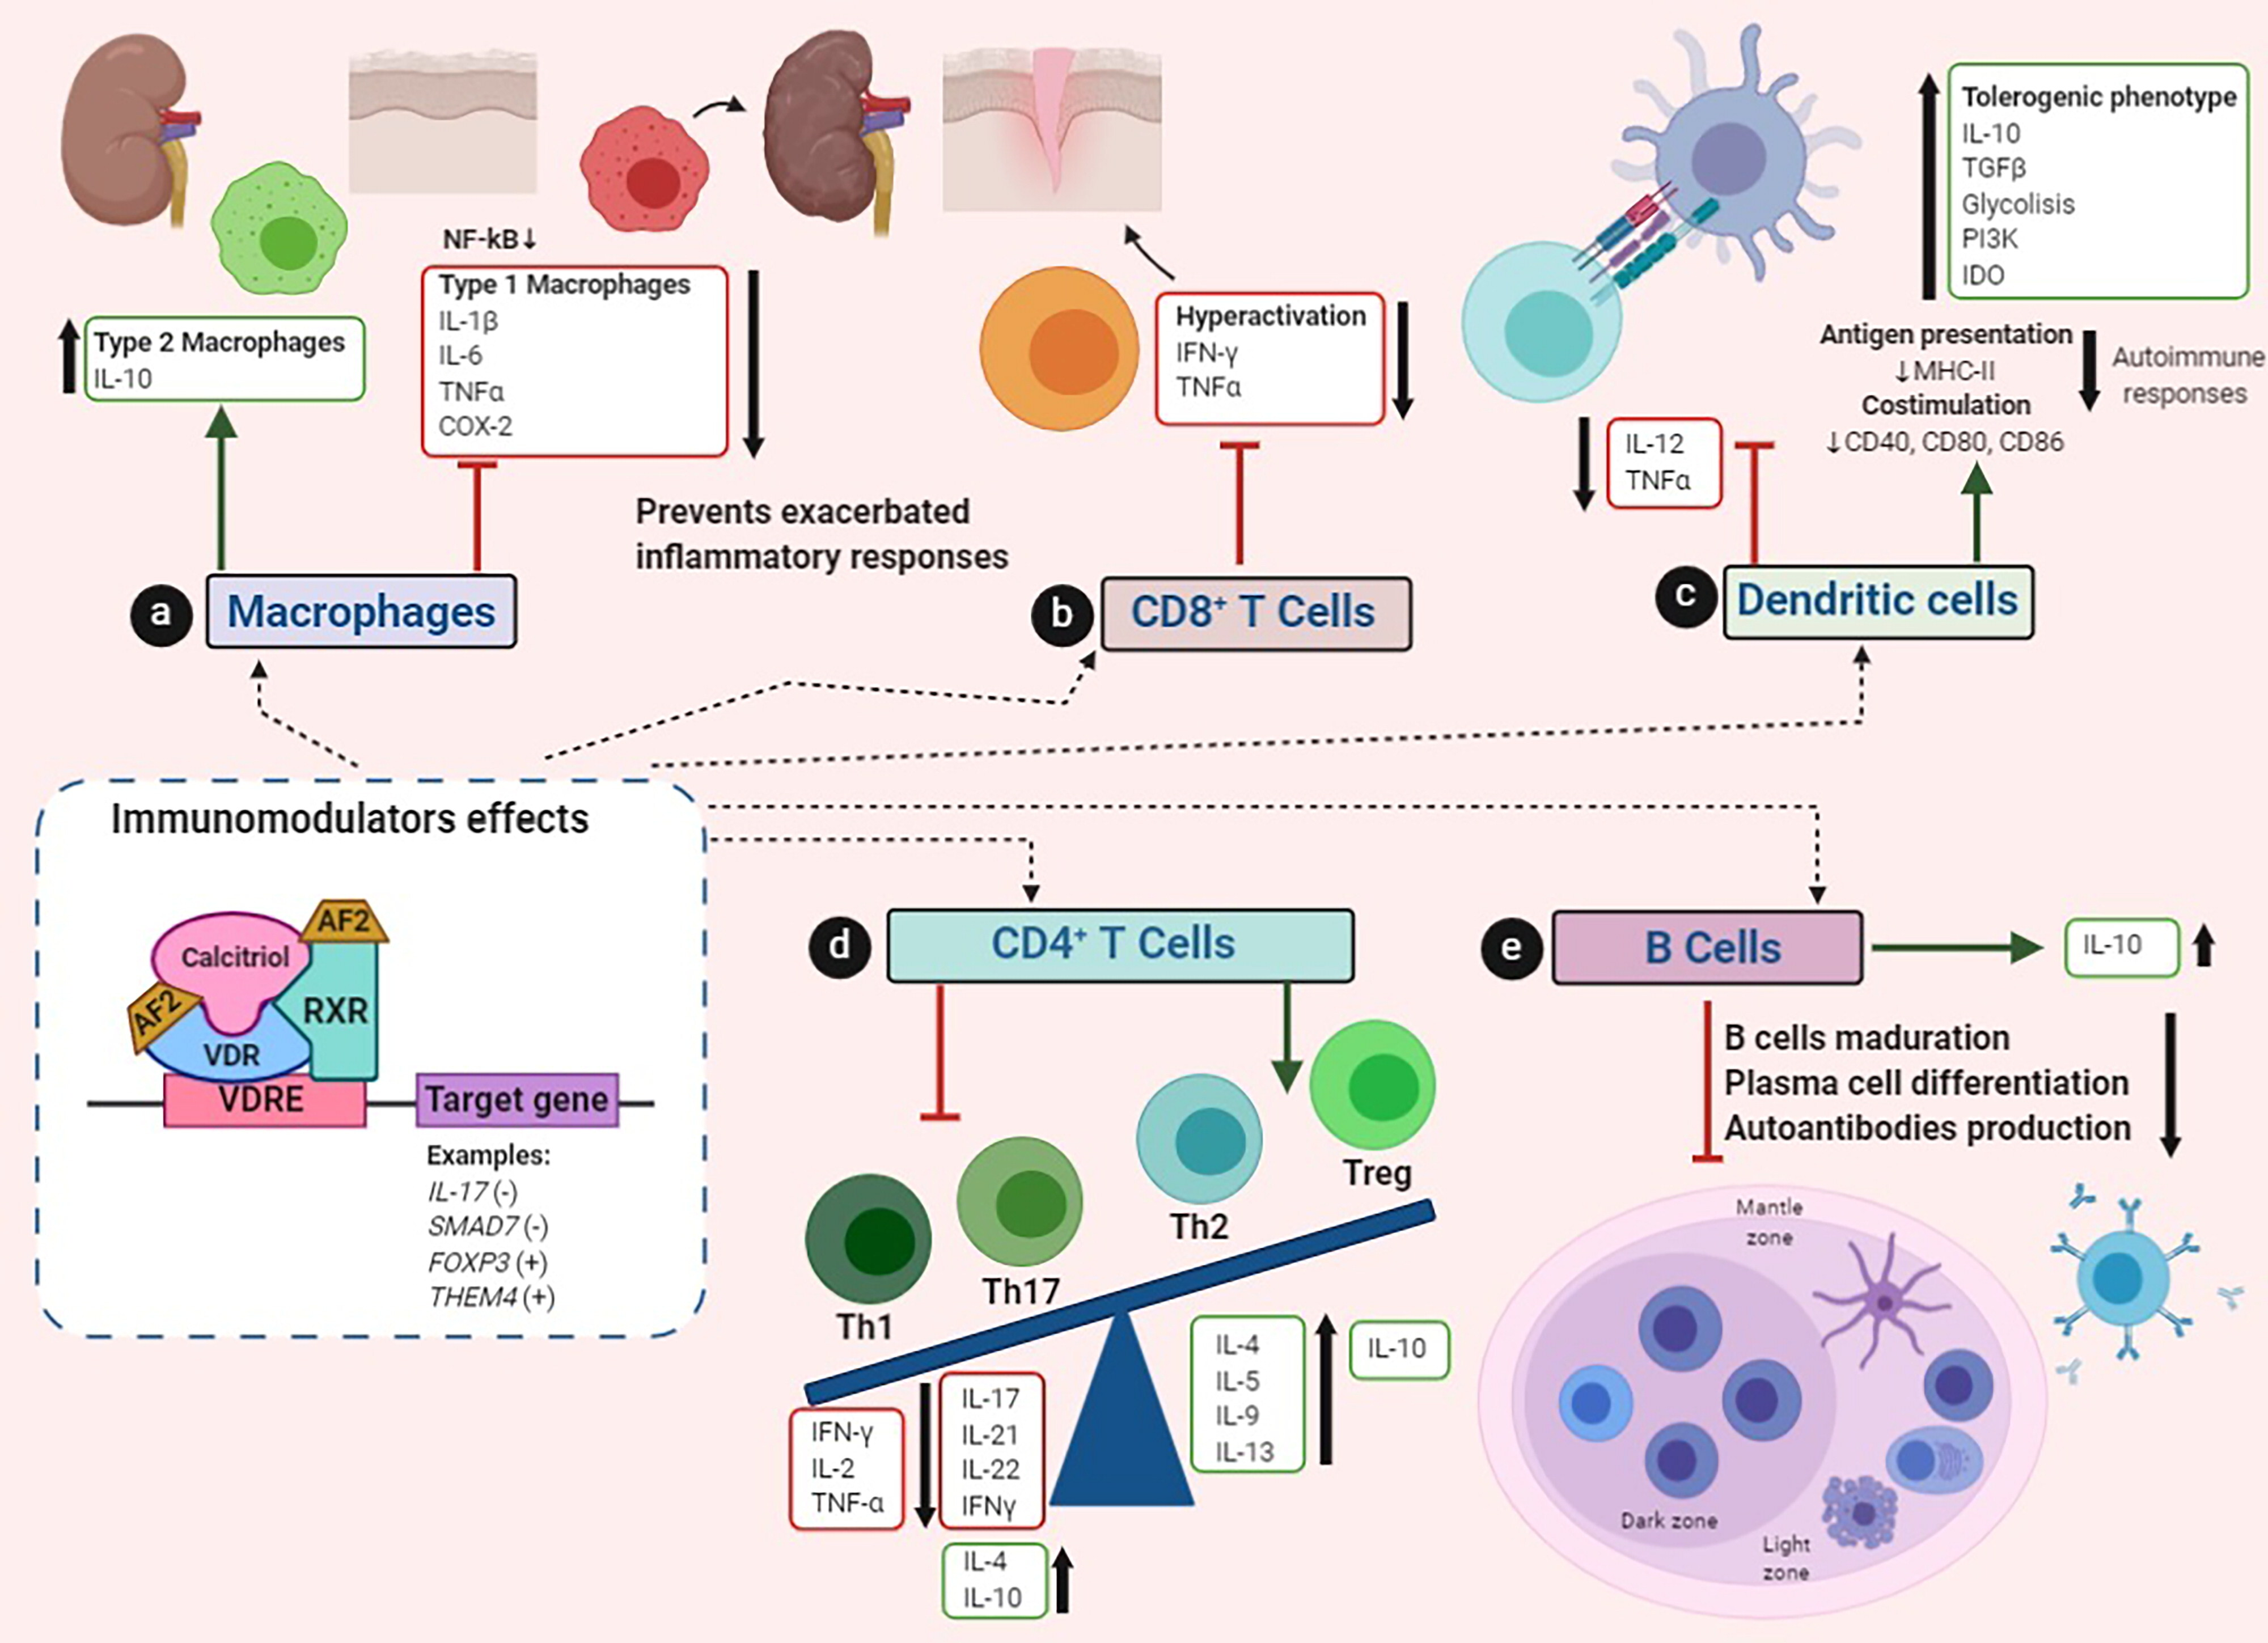
\includegraphics{figures/calcitriol-immunomodulatory.jpg}

}

\caption[Schéma récapitulatif des effets immunomodulateurs du
calcitriol.]{\label{fig-immunomod}\textbf{Schéma récapitulatif des
effets immunomodulateurs du calcitriol.} Le calcitriol se fixe sur le
VDR qui en interagissant avec le VDRE provoque une transcription de
gènes régulateurs de l'immunité, conduisant à des effets globalement
favorisant la suppression et tolérance immunitaire. Cette modulation se
manifeste directement par l'inhibition de facteurs cytokines
pro-inflammatoires et l'augmentation de cytokines anti-inflammatoires ou
indirectement en favorisant le phénotype de cellules immunes
immunosuppressives comme les macrophages de type M2, les sous-types de
lymphocytes Th\textsubscript{2} et T\textsubscript{reg} ou le phénotype
tolérogénique des cellules dendritiques. \textcite{Meza-Meza.2022}}

\end{figure}%

\subsection{Implications de la vitamine D dans la réponse immunitaire
antivirale}\label{implications-de-la-vitamine-d-dans-la-ruxe9ponse-immunitaire-antivirale}

Les études démontrent globalement que la vitamine D augmente l'immunité
antivirale et en particulier la réponse innée immune, et inhibe les
réponses cytokiniques pro-inflammatoires. La vitamine D possède une
implication dans la réponse immunitaire antivirale car de nombreux virus
respiratoires ciblent les cellules épithéliales pulmonaires, qui sont
très sensibles à la présence de vitamine D. Les cellules épithéliales
induisent fortement le \ac{CYP27B1} lors de présence du calcidiol ainsi
que lors de la détection d'ARN viraux double brins
\autocite{Bishop.2021}. La réponse antivirale innée passe en partie par
l'activation des \acp{TLR}, qui cause la uprégulation du CYPB27B1 et du
VDR, médié par l'activation du TLR2, induisant par la suite l'expression
de \emph{CAMP} \autocite{Liu.2006}. La vitamine D est ainsi un très fort
inducteur du gène \emph{CAMP} qui transcrit le peptide antimicrobien
cathélicidine LL-37 capable de se lier aux \ac{LPS} et de causer la
perméabilisation des membranes, ainsi que celui de CD14. En effet, le
CD14 est le cofacteur du TLR4 qui permet de reconnaître classiquement le
LPS. Le calcitriol inhibe également le signalement du facteur
pro-inflammatoire \ac{nfkb} dans les cellules pulmonaires
\autocite{Bishop.2021}.

La vitamine D régule la production d'interférons et module la fonction
des cellules immunitaires antivirales ainsi qu'en induisant la
production de peptides antimicrobiens. En effet, elle stimule la
production des AMPs, \emph{CAMP}, \emph{HBD2}, \emph{DEFB4}, dont les
deux derniers éléments contiennent/permettent la génération du complexe
\ac{VDRE} \autocite{Bishop.2021}.

Les réponses transcriptionnelles initiales ayant lieu lors d'une
infection virale concernent en particulier les membres de la famille des
facteurs de régulation de l'interféron tels que IRF3 et IRF7, les
membres de la famille AP-1 et \ac{nfkb}. Le calcitriol agit en inhibant
le \ac{nfkb} qui est un puissant pro-inflammatoire, grâce à l'induction
de \ac{IKBa} \autocite{Bishop.2021}.

Un mécanisme clé de la réponse antivirale médiée par la vitamine D est
l'induction puissante de l'expression de \emph{CAMP} via le TLR2, gène
codant pour la forme active de la cathélicidine LL-37 qui va à son tour
favoriser la détection des ARN viraux double brins par le \ac{PRR} TLR3.
Le LL-37 peut se lier à l'ARN double brin viral qui se retrouve dans les
endosomes, où est situé le TLR3. Le TLR3 est un \ac{PRR} important dans
la reconnaissance du virus, et enclenche à son tour l'activation du
mécanisme immunitaire inné, en passant par le \ac{nfkb}. Les études
montrent également que le LL-37 possède une activité antivirale directe
qui perturbe les membranes virales \autocite{Bishop.2021}. Une étude
montre que lorsque la concentration de vitamine D est insuffisante, ou
lorsqu'un anticorps anti-LL37 est utilisé afin de bloquer l'effet de la
forme active de la cathélicidine, l'activité antivirale observé dans les
poumons est bloqué, et la supplémentation en vitamine D restaure le
pouvoir antiviral de LL-37 \autocite{Buonfiglio.2017}. Il est
intéressant de noter que cette induction de \emph{CAMP} dépend de la
concentration en calcidiol, et une concentration insuffisante ne permet
pas une induction en CAMP, ce qui renforce l'importance d'une
concentration adéquate en vitamine D appropriée pour le système
immunitaire \autocite{White.2022}.

Le calcitriol est capable d'induire NOD2 qui induit l'autophagie pour
augmenter la clairance virale. L'autophagie est un mécanisme clé dans le
contrôle de la réplication et l'infection virale, permettant la
dégradation des composants intracellulaires, y compris les protéines
virales et les acides nucléiques. En effet, le calcitriol induit
directement l'expression d'enzymes clés de l'autophagie comme Beclin1 et
PI3KC. en favorisant la cathélicidine qui induit Beclin1. Il peut
également favoriser indirectement l'autophagie en supprimant
l'inhibition de l'autophagie par la voie de signalisation mTOR, et en
stimulant le calcium intracellulaire et le \ac{NO} par le calcitriol
afin d'augmenter l'activité de PI3KC3 \autocite{Bishop.2021}.

\subsection{Action paracrine et
intracrine}\label{action-paracrine-et-intracrine}

{[}\emph{Peut-être une partie sur ce mécanisme ? Cela me semble
important car la question de la dose minimale efficace pour les effets
du calcitriol sur le système immunitaire dépend de cette concentration
locale à effet paracrine qui ne peut être mesurée uniquement dans une
recherche in vitro, alors que la dose typiquement mesurée chez la
population constitue le calcidiol sanguin}{]}

Dose utilisée dans l'essai in vitro de \textcite{Hewison.2007} de 5, 50
and 150 nM. Ces valeurs ont été choisies pour représenter les conditions
de carence en vitamine D, d'insuffisance en vitamine D et de suffisance
en vitamine D, respectivement.

\section{Dose de vitamine D nécessaire à
l'immunité}\label{dose-de-vitamine-d-nuxe9cessaire-uxe0-limmunituxe9}

{[}\emph{Pourquoi est-ce que 4000 UI est une des doses minimales
recommandées pour un effet immunitaire ? Pourquoi est-ce que le seuil de
``40 ng/mL'' est important pour cet effet suffisant ?}{]}

\newpage{}

\chapter{Vitamine D et COVID-19}\label{vitamine-d-et-covid-19}

\section{Physiopathologie de la COVID-19 concernant le système
immunitaire}\label{physiopathologie-de-la-covid-19-concernant-le-systuxe8me-immunitaire}

\begin{itemize}
\item
  La \ac{COVID-19} est causée par le virus \ac{SARS-CoV-2} qui est un
  virus à ARN simple brin enveloppé qui appartient à la famille des
  Coronaviridae. Le virus envahit l'organisme par le biais de la
  protéine de pointe appelée spike protein (S). La protéine de pointe
  est impliquée dans la liaison aux récepteurs de surface des cellules
  hôtes, notamment l'\ac{ACE2}, qui est notamment impliquée dans le
  \ac{SRAA}.
\item
  Lorsque la réponse inflammatoire innée et adaptative ne devient plus
  protectrice mais devient exacerbée, associée à une réplication virale
  non controllée et des cellules infectée non éliminée, la réponse
  immunitaire se perpétue et s'aggrave, entraînant un \ac{SDRA} ou une
  \ac{CIVD} \autocite{Contreras-Bolívar.2023}.
\end{itemize}

\subsection{Processus d'infection : entrée dans les cellules hôtes,
réplication
virale}\label{processus-dinfection-entruxe9e-dans-les-cellules-huxf4tes-ruxe9plication-virale}

Le \ac{SARS-CoV-2} utilise sa protéine de pointe pour se fixer à la
surface des cellules respiratoires humaines. Une fois attaché à
\ac{ACE2}, le virus fusionne avec la membrane cellulaire, permettant
ainsi son entrée dans la cellule. Une fois à l'intérieur de la cellule,
le génome viral est libéré, et le virus commence à se répliquer en
utilisant les ressources de la cellule hôte. La réplication virale
aboutit à la production de nombreuses particules virales qui peuvent
infecter d'autres cellules, propageant ainsi l'infection dans le tissu
pulmonaire et au-delà.

Après fusion des membranes virales et cellulaires, le SARS-CoV-2 pénètre
et infecte les cellules épithéliales et les pneumocytes de type II. La
liaison de la protéine S virale avec l'\ac{ACE2} entraîne la sécrétion
de cytokines (TNF-α, IL-1, IL-6, chimiokines), ce qui provoque une
hyperperméabilité́ capillaire ainsi que l'attraction d'\ac{IFN-1} et de
cellules inflammatoires.

\subsection{Réponse immunitaire innée et adaptative face à
l'infection}\label{ruxe9ponse-immunitaire-innuxe9e-et-adaptative-face-uxe0-linfection}

Lorsque le SARS-CoV-2 infecte les cellules respiratoires, il déclenche
une série de réponses immunitaires impliquant d'abord des cellules
immunitaires innées telles que les macrophages et les cellules
dendritiques qui détectent la présence du virus. La réponse innée
entraîne la production de cytokines pro-inflammatoires pour attirer
davantage de cellules immunitaires sur le site de l'infection par le
biais de chimiokines tel que l'\ac{IL-8} et le MCP-1 qui attirent les
neutrophiles, granulocytes et monocytes.

Simultanément, le système immunitaire adaptatif est mobilisé. Les
lymphocytes T cytotoxiques (CD8\textsuperscript{+}) identifient et
détruisent les cellules infectées par le virus, limitant ainsi la
propagation du \ac{SARS-CoV-2}. Les lymphocytes B produisent des
anticorps spécifiques qui peuvent neutraliser le virus. Ensemble, ces
deux composantes de la réponse immunitaire contribuent à contrôler
l'infection.

\section{Rationnel du mécanisme physiologique de l'usage de la vitamine
D dans la
COVID-19}\label{rationnel-du-muxe9canisme-physiologique-de-lusage-de-la-vitamine-d-dans-la-covid-19}

\textcite{Borsche.2021}: La vitamine D agit sur deux principaux
évènements mettant le pronostic vital en jeu dans la physiopathologie de
la COVID-19: \ac{ARDS} et \ac{CRS}, par un mécanisme particulier
spécifique entre la vitamine D et le SARS-CoV-2 : Dans le système rénine
angiotensine aldostérone :

\begin{itemize}
\tightlist
\item
  la vitamine D agit comme modulateur du \ac{SRAA} en diminuant la
  rénine et en augmentant ACE2
\item
  La diminue ATII et augmente Ang(1-7) ce qui favorise la voie MasR.
\end{itemize}

Selon \textcite{Borsche.2021}, il existe 5 mécanismes par lesquels la
vitamine D supporte le système immunitaire :

\begin{itemize}
\tightlist
\item
  Diminution de production de Th1
\item
  Diminution du \ac{CRS} (cytokine release syndrome)
\item
  Induction de la production de LL-37 (cathélicidine), peptide
  antimicrobien (papier sur l'importance de la cathélicidine dans la
  COVID-19)
\item
  Modulation de la fonction endothéliale et de la perméabilité
  vasculaire
\item
  Réduction des anomalies de la coagulabilité dans les patients COVID-19
\end{itemize}

\subsection{Système Rénine Angiotensine
Aldostérone}\label{systuxe8me-ruxe9nine-angiotensine-aldostuxe9rone}

\begin{itemize}
\item
  \emph{La physiopathologie de la COVID-19 implique le} \ac{SRAA}
  \emph{causé par l'entrée du virus dans les cellules ce qui provoque
  l'endocytose du récepteur-enzyme ACE2 et inhibant ainsi ses
  fonctions.} ACE2 est une enzyme importante dans le \ac{SRAA}, qui
  possède un effet antagoniste du récepteur ACE, les deux agissant comme
  une balance afin de réguler diverses fonctions physiologiques telles
  que la pression artérielle, l'inflammation, la fibrose, la
  prolifération cellulaire, la régénération tissulaire, et la réponse
  immunitaire \textbf{(Figure~\ref{fig-ace2-masR})}
  \autocite{Brojakowska.2020}.
\item
  De plus, la bradykinine, régulée par ACE, est impliquée dans les
  processus perturbés par la COVID-19. ACE est responsable de la
  dégradation de la bradykinine, qui est impliquée dans le système
  bradykinine, régulant la pression artérielle, induisant la
  vasodilatation, natriurèse et hypotension
  \textbf{(Figure~\ref{fig-ace2-masR})}. La bradykinine serait également
  lors de l'inflammation car elle induit le recrutement des neutrophiles
  et une augmentation de la perméabilité vasculaire. L'analyse de
  \textcite{Garvin.2020} révèle une ``tempête bradykinique'', où
  l'expression de bradykinine chez les patients COVID-19 est en
  surreprésentation par rapport aux patients contrôles. De plus,
  l'expression de ACE2 est également surreprésentée chez les patients
  COVID-19, ce qui implique une régulation négative de ACE par ACE2,
  conduisant à une augmentation de la bradykinine. L'augmentation de
  bradykinine induit une vasodilatation et une perméabilité vasculaire.
  La tempête bradykinique explique la plupart de la symptomatologie de
  la COVID-19 \autocite{Garvin.2020}..
\end{itemize}

\begin{figure}

\centering{

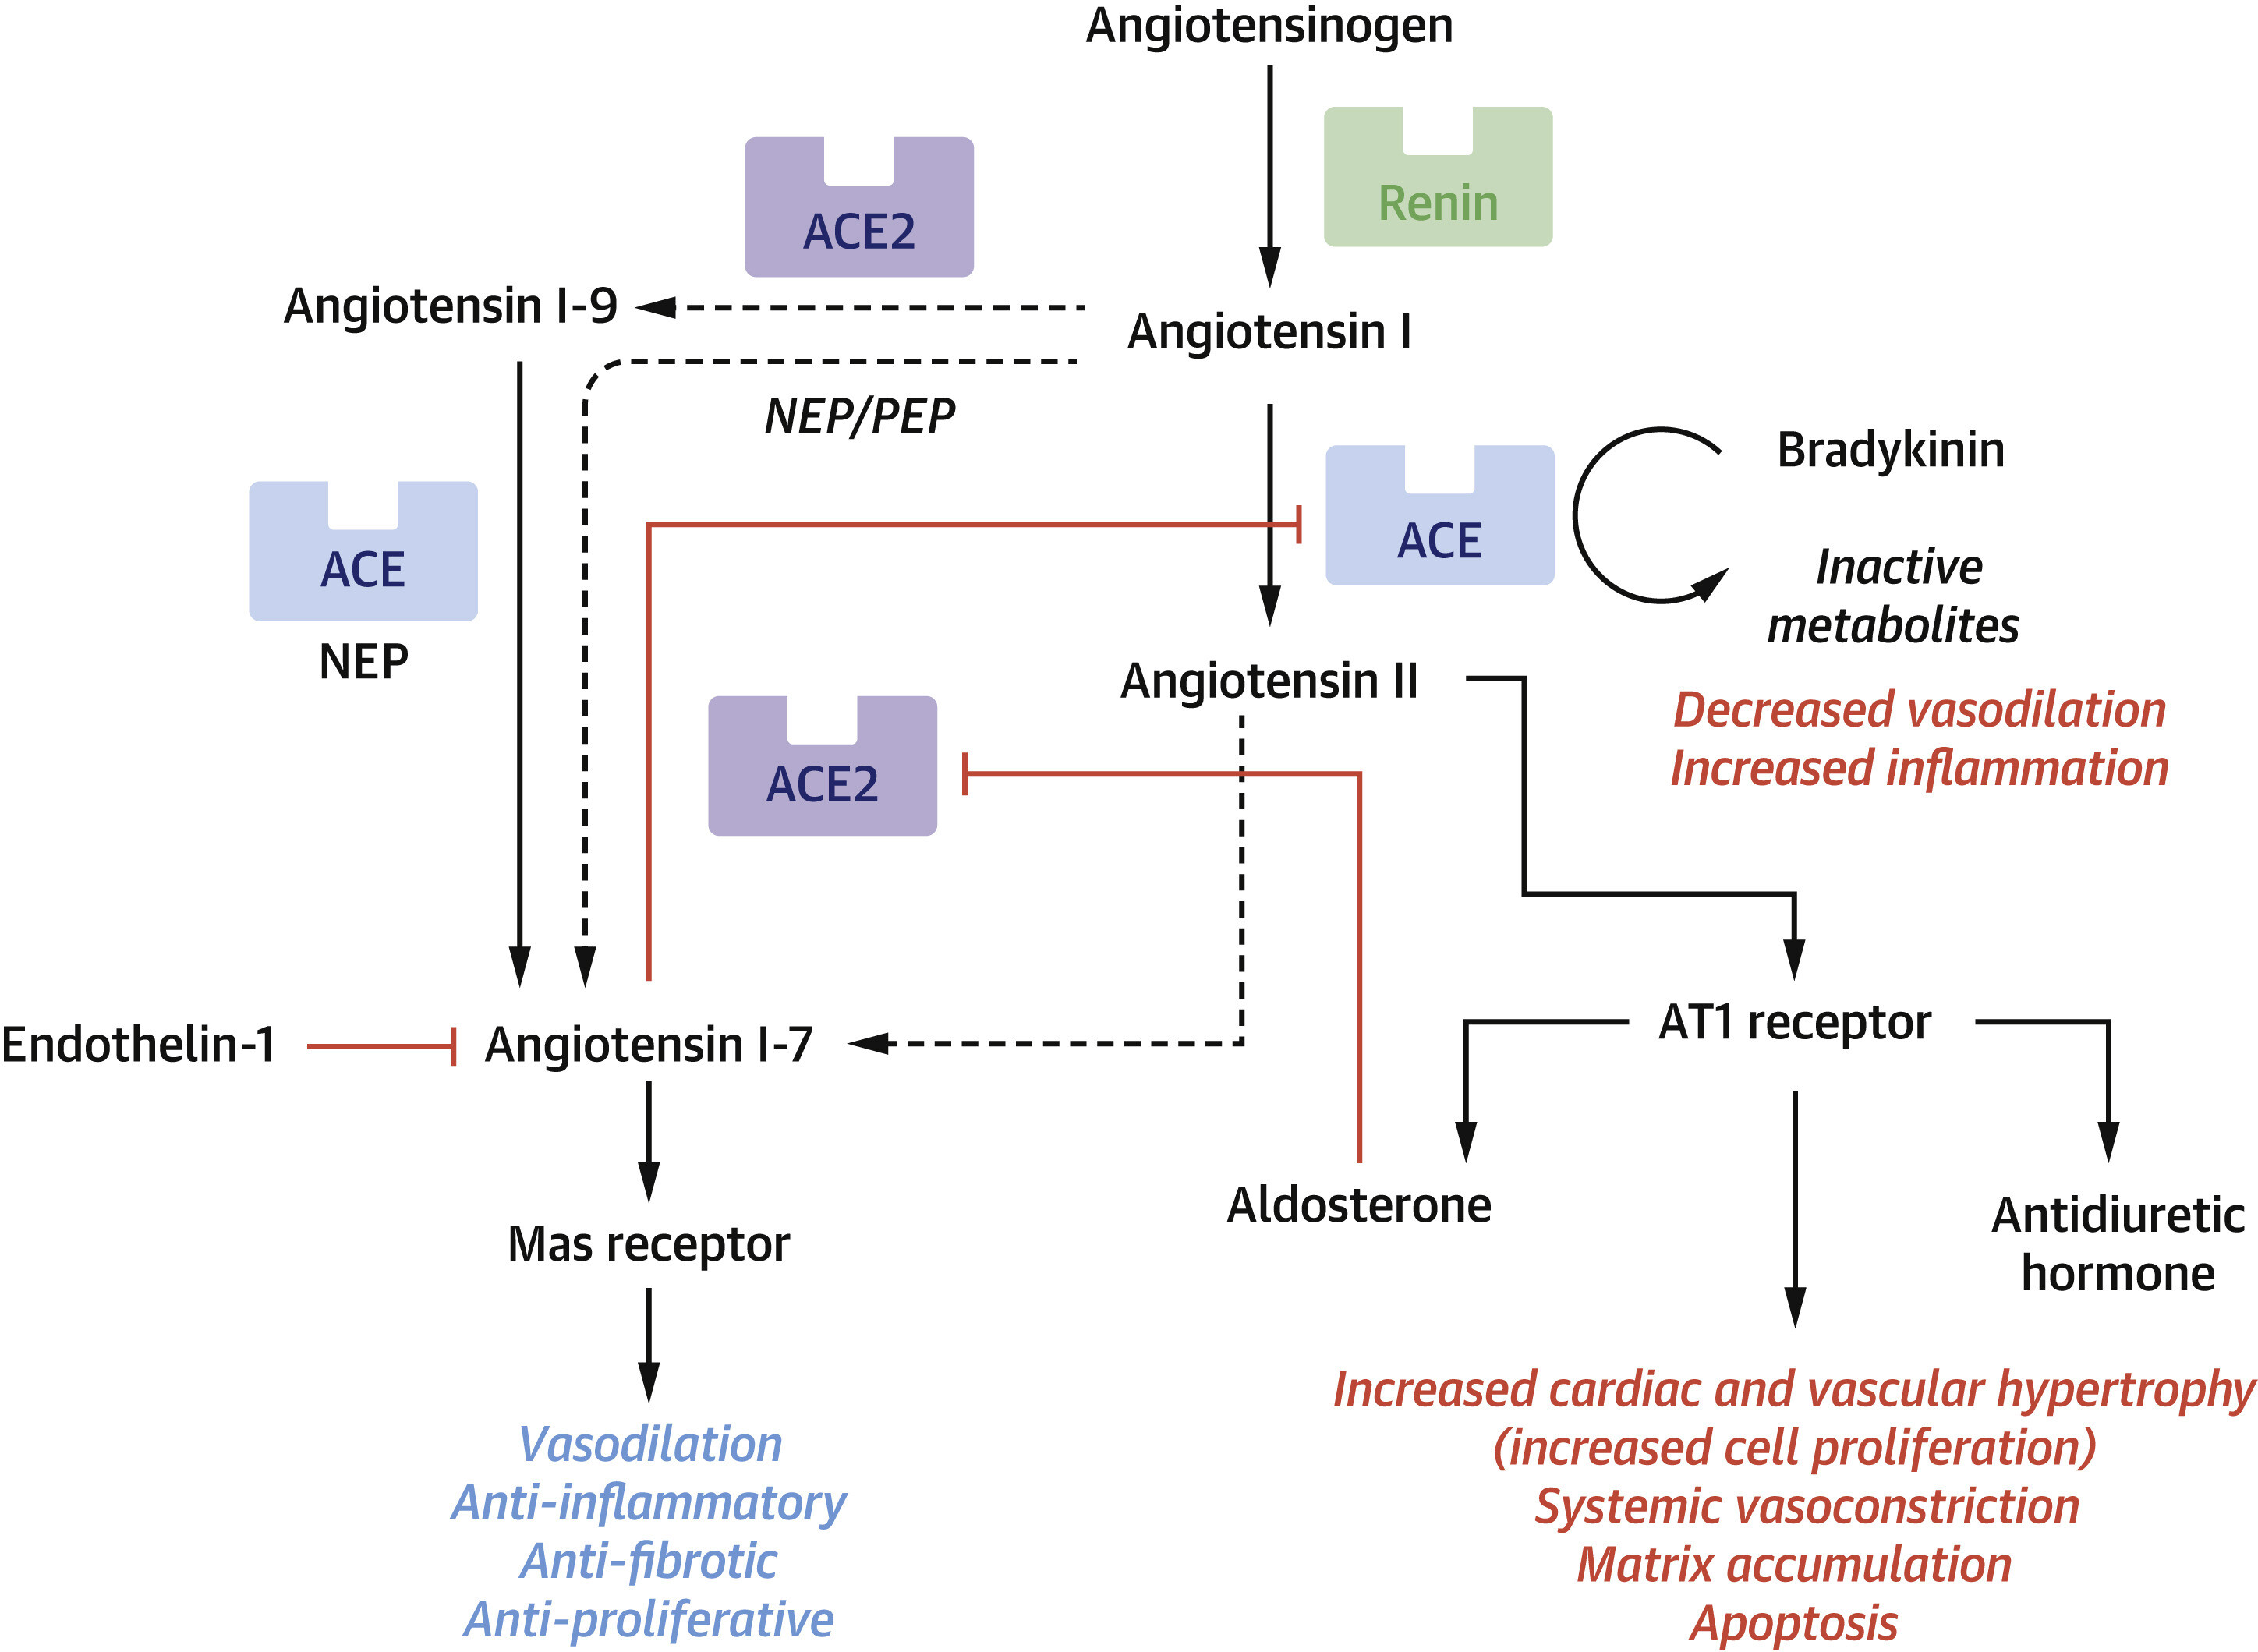
\includegraphics{figures/Brojakowska-RAS-ACE2-Regulation.jpg}

}

\caption[Régulation du SRAA et de l'axe
ACE2/Ang-1-7/AT1/MasR]{\label{fig-ace2-masR}Régulation du SRAA et de
l'axe ACE2/Ang-1-7/MasR \autocite{Brojakowska.2020}.}

\end{figure}%

\begin{itemize}
\item
  Puisque la \ac{COVID-19} est caractérisée souvent par une
  hyperinflammation non résolue (source), associé à une infection aiguë
  des poumons, et que la majorité des personnes sont déficientes en
  vitamine D (Section~\ref{sec-statut-vd}), la vitamine D étant liée à
  la régulation de l'inflammation, et ayant possiblement des bénéfices
  sur les infections pulmonaires, l'usage hypothétique de la vitamine D
  pourrait être utile dans la \ac{COVID-19} en renforçant le système
  immunitaire contre l'infection virale pulmonaire, tout en permettant
  au système immunitaire de pouvoir basculer du programme
  d'hyperinflammation vers un équilibre immunitaire plus tolérogène.
\item
  \textcite{Li.2002} ont établi une relation entre la rénine et le
  système rénine-angiotensine-aldostérone. La vitamine
  D\textsubscript{3} a été observée comme étant un régulateur négatif du
  \ac{SRAA}.

  \begin{itemize}
  \item
    Li et al.~(2002) : VDR KO = augmentation activité SRAA. VitD
    =\textgreater{} diminution de rénine.
  \item
    En effet l'augmentation des niveaux de vitamine D le niveau de
    rénine, ce qui entraîne une downrégulation du \ac{SRAA} chez
    l'animal et l'homme \autocite{Li.2004,Schwalfenberg.2007}. Il peut
    induire l'activité de l'axe anti-inflammatoire ACE2/Ang-(1-7)/MasR
    et inhiber la rénine et l'axe pro-inflammatoire ACE/Ang II/AT1R,
    augmentant ainsi l'expression et la concentration de l'ACE2, du MasR
    et de l'Ang-(1-7). La voie médiée par \ac{ACE2} favorise une
    diminution de l'apoptose, de la fibrose et de l'inflammation tandis
    que la voie médiée par ACE et AT1 possède une action opposée.
  \end{itemize}
\item
  Extrapolation :

  \begin{itemize}
  \item
    Lin et al68 observed that calcitriol decreased ACE concentration and
    ACE/ACE2 ratio and enhanced ACE2 concentration in diabetic rats.
  \item
    Accordingly, administration of the synthetic vitamin D analog,
    paricalcitol, led to increased levels of ACE2 in tubular cells and
    decreased levels of ACE2 within the circulation in an animal model
    of type I diabetes, thereby slowing the development of diabetic
    nephropathy.
  \item
    Le mécanisme du fonctionnement du SRAA et de l'action de la vitamine
    D sur le SRAA est similaire entre les maladies.
  \end{itemize}
\item
  Puisque le \ac{SRAA} est impliqué dans la COVID-19 aussi bien dans la
  régulation de l'inflammation et du maintien du système
  cardiovasculaire que dans la perturbation de ceux-ci par l'entrée du
  virus dans les cellules par le biais de \ac{ACE2}, réduisant ainsi
  l'expression de \ac{ACE2}, conduisant à des lésions pulmonaires et une
  pneumonie, la vitamine D pourrait avoir un effet bénéfique en agissant
  sur le \ac{SRAA}.
\end{itemize}

\autocite{Mahdavi.2020}

\begin{itemize}
\tightlist
\item
  \textcite{Shiravi.2022} : RAS pathway can also be down-regulated by VD
  which may prevents the cardiovascular complications induced by
  COVID-19.
\end{itemize}

!{[}\textbf{Schéma du rôle du la vitamine D dans l'inhibtion du
SRAA.}(figures/borsche.2021-vd-ras.jpg)\{\#fig-vd-ras fig-scap=``Schéma
du rôle du la vitamine D dans l'inhibition du SRAA.''\}

\autocite{Chauss.2022} : Autocrine vitamin D signaling switches off
pro-inflammatory programs of TH1 cells{]}

\subsection{Mécanisme lié l'inhibition de
l'hyperinflammation}\label{muxe9canisme-liuxe9-linhibition-de-lhyperinflammation}

SARS-CoV-2, the viral cause of COVID-19, leads to lethal infection with
multiple organ damages, particularly in the respiratory and
cardiovascular tracts, through upregulation of the RAS pathway and
inducing a cytokine storm.

\subsection{Effet antioxydant}\label{effet-antioxydant}

\begin{itemize}
\tightlist
\item
  \textcite{Shiravi.2022} : VD also has antioxidant effects through
  modulating the mitochondrial activities, upregulating of glutathione,
  glutathione peroxidase and superoxide dismutase, and down-regulating
  the NADPH oxidase.
\end{itemize}

\subsection{Mécanisme antiviral induit par la vitamine D contre la
COVID-19}\label{muxe9canisme-antiviral-induit-par-la-vitamine-d-contre-la-covid-19}

\begin{itemize}
\item
  En interagissant avec le VDR qui se trouve sur les cellules
  immunitaires (cellules B, cellules T et cellules présentatrices
  d'antigènes) et les cellules épithéliales pulmonaires, le complexe
  calcitriol - VDR induit l'expression transcriptionnelle de peptides
  anti-microbiens tels que les cathélicidines et les défensines. Les
  cathélicidines servent à perturber les membranes cellulaires
  bactériennes, ainsi que les virus enveloppés tels que le SRAS - CoV -
  2, tandis que les défensines favorisent le chimiotactisme des cellules
  inflammatoires par le biais d'une perméabilité capillaire accrue.
  \autocite{Munshi.2021}
\item
  Vitamin D and its metabolites have immunomodulatory effects via the
  development of the immune cells, anti-inflammatory effects, and
  production of some anti-microbial molecules such as defensins and
  cathelicidins \autocite{Shiravi.2022}.
\end{itemize}

Une étude menée par \textcite{Chauss.2022} examine les mécanismes
moléculaires qui conduisent à la rétractation et à l'arrêt du phénotype
CD4\textsuperscript{+} \ac{Th1}. Les analyses issues du single cell
RNA-sequencing (scRNA-Seq) ont permises de mettre en évidence que le
complément induisait l'expression de \ac{VDR} et de \ac{CYP27B1},
permettant aux cellules d'utiliser la vitamine D. La vitamine D permet
ainsi de faire passer le phénotype pro-inflammatoire \ac{Th1} au
phénotype anti-inflammatoire IL-10\textsuperscript{+}.

Il est intéressant de noter la vitamine D a permise d'induire l'IL-6,
qui possède dans ce cas un rôle immunomodulateur contrairement au rôle
standard de pro-inflammation. \autocite{Chauss.2022}

\textcite{Bishop.2021}

\section{Statut en vitamine D, épidémiologie du risque infectieux en
général et COVID-19 en particulier}\label{sec-statut-vd}

\begin{itemize}
\item
  La majorité de la population possède un statut en vitamine D même
  insuffisant pour des effets bénéfiques à visée osseuse (inférieur à 20
  ng/mL). De plus, les personnes âgées supérieurs à 70 ans qui sont à
  plus fort risque de symptômes sévères sont souvent déficitaires en
  vitamine D comparés aux personnes plus jeunes.
\item
  Selon \textcite{Borsche.2021}, la méta-analyse des 8 études analysées
  rapporte une médiane de 23,2 ng/mL. Les régressions mathématiques de
  deux bases de données séparées montrent que le taux de mortalité
  diminue à partir de 30 ng/mL, et un seuil de 50 ng/mL serait optimal
  pour diminuer la mortalité liée à la COVID-19.
\item
  L'étude de \textcite{Kaufman.2020} : Sur 191 779 patients, 39 190
  (12,5\%) sont positifs au COVID-19 avec \textless{} 20 ng/mL, 27 870
  patients (8,5\%) avec 30-34 ng/mL (8,1\%) et 12 321 (5,9\%) patients
  positifs \textgreater= 55 ng/mL Le minimum d'infection est observé
  pour un taux de 55 ng/mL.
\end{itemize}

\begin{figure}

\centering{

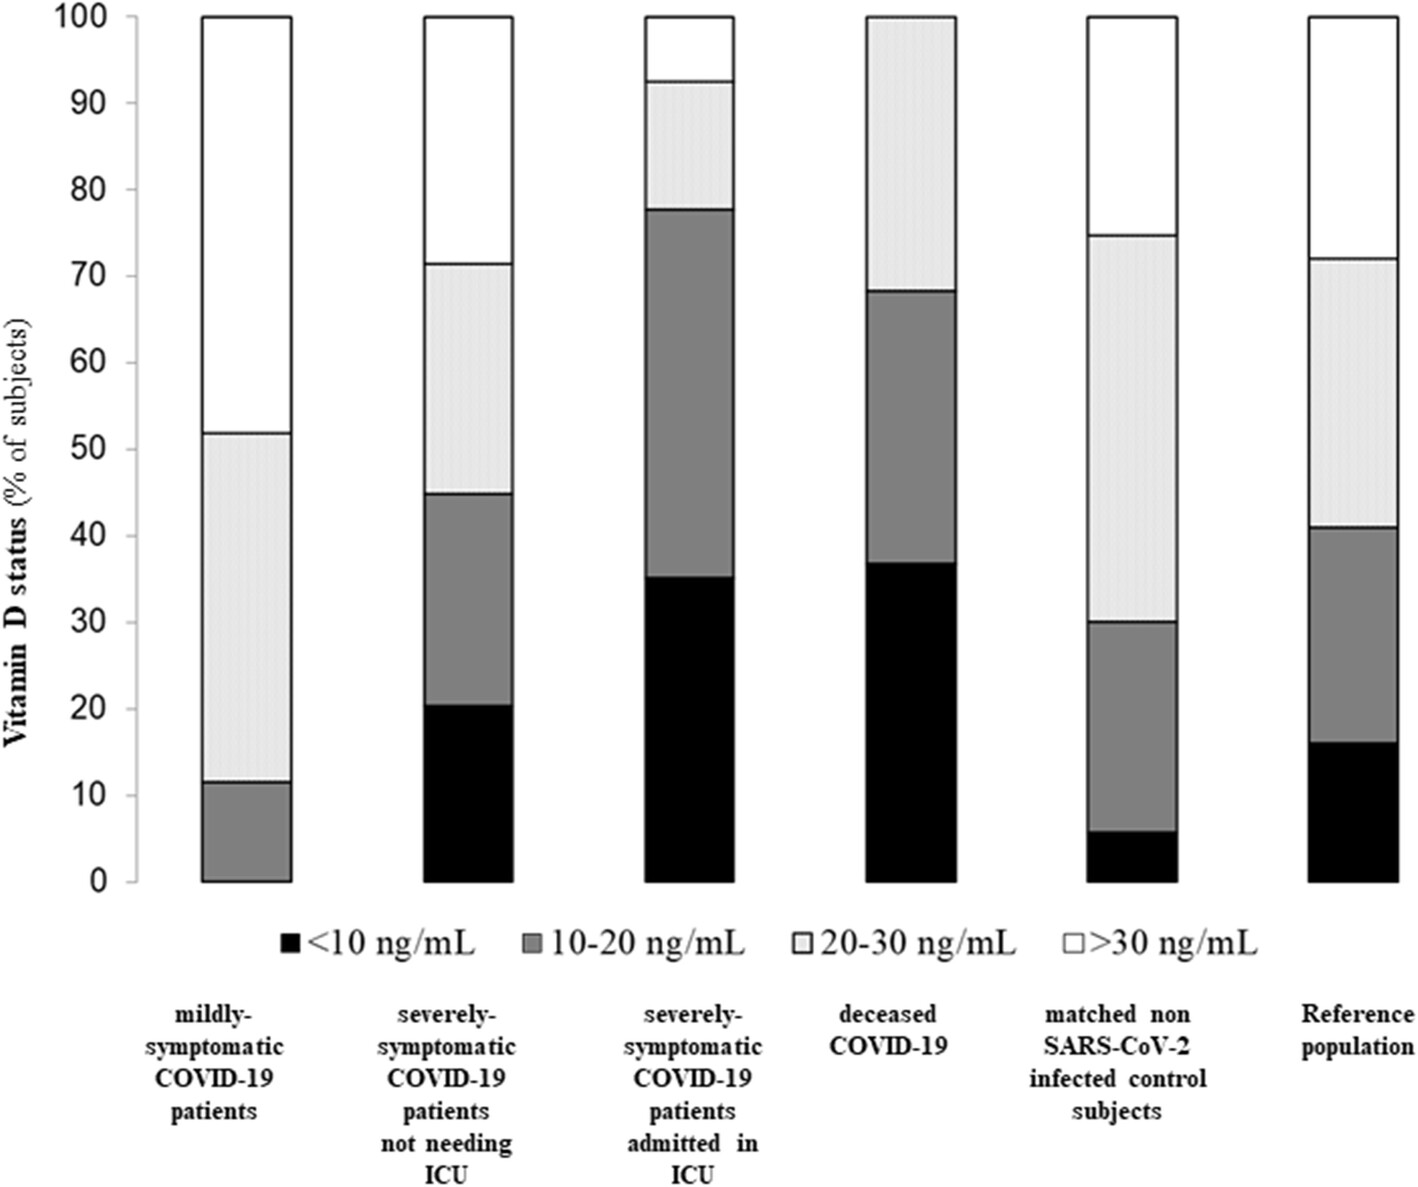
\includegraphics{figures/Campi.2021-Prevalence_rates_of_vitamin_D_insufficiency_or_deficiency.jpg}

}

\caption[Taux de prévalence de l'insuffisance ou de la carence en
vitamine D]{\label{fig-vd-covid-deficiency}Taux de prévalence de
l'insuffisance ou de la carence en vitamine D \autocite{Campi.2021}.}

\end{figure}%

\section{Etudes observationnelles}\label{etudes-observationnelles}

\begin{itemize}
\item
  \textcite{Oristrell.2022} : Cohorte rétrospective en Espagne de
  108,343 patients, les auteurs ne trouvent pas d'association entre la
  supplémentation en vitamine D. Mais patients \textgreater{} 30 ng/mL =
  baisse de mortalité, sévérité et risque d'infection. L'étude est
  analysée par \textcite{Sartini.2024}\\
\item
  \textcite{Munshi.2021} : Méta-analyse sur 5 études rétrospective et 1
  étude de cas (2020). N = 376 patients, moyenne = 8.76 ng/mL.
  Standardized mean difference = -0.58 ; On observe de grandes
  différences pour des critères de sévérité (SMD = -0.50) et encore plus
  lors d'admission aux urgences (SMD = -0.84) en particulier. {[}Etude
  compliquée à analyser et peut-être faible taux de preuve?{]}
  =\textgreater{} Hypovitaminose D associée à un mauvais pronostic pour
  les patients COVID-19.
\item
  \textcite{Campi.2021} : un faible taux de vitamine D est associé à un
  risque accru d'être hospitalisé, d'admission en soins intensifs.
  Plusieurs études associent une déficience sévère (\textless{} 5 ng/mL)
  à un risque accru de mortalité Figure~\ref{fig-vd-covid-deficiency}
\item
  \textcite{Pal.2021} : Etude rétrospective sur 72 patients : les
  patients admis à l'hôpital pour un cas de COVID-19 non sévère ont une
  moyenne de 9.8 ng/mL soit une hypovitaminose D (97\% des patients), et
  également une hypocalcémie (67\%).
\item
  Les études écologiques rapportent également une différence de
  concentration de vitamine D entre les patients COVID-19 positifs et
  négatifs (10.8 nmol/L vs 20.8 nmol/L \autocite{Baktash.2021}). En
  effet, il existe une corrélation positive entre l'incidence de
  COVID-19 et le taux de déficience en vitamine D (R = 0.36), la
  fatalité (R = 0.40) et de mortalité (R = 0.38). Le pourcentage médian
  de déficience de vitamine D est de 49\%, indiquant que le 23ème pays
  parmi les 46 pays analysés, possède une déficience en vitamine D de
  49\% \autocite{Mariani.2021}. Une étude d'un centre hospitalier
  rapporte que chez le groupe de patients considéré vitamine D déficient
  (\textless{} 12 ng/mL) contre non déficient (\textgreater{} 12 ng/mL),
  il existe une association entre la déficience de vitamine D et le
  risque de ventilation mécanique invasive et de mortalité (HR = 6.12 et
  14.73 respectivement) \autocite{Radujkovic.2020}.
\end{itemize}

Données contradictoires avec d'autres études observationnelles et RCTs:
- \textcite{Hernández.2020} : 197 patients COVID-19 vs 197 contrôles,
25OHD = 13.8 ng/mL vs 20.9 ng/mL, mais pas d'associations avec la
sévérité ou mortalité. - \textcite{Jevalikar.2021}: 48.2 \% des 410
patients ont un taux de vitamine D \textless{} 20 ng/mL, mais pas
d'association avec la sévérité, mortalité, admission hospitalière,
oxygénothérapie et pas de corrélation avec les marqueurs inflammatoires
(IL-6, CRP). - \textcite{Cereda.2021} : La supplémentation moyenne
\textgreater{} 1800 UI/jour ne donne pas de différence par rapport au
groupe non supplémenté en terme d'hospitalisation.
-\textcite{Murai.2021} : {[}Pas d'article en libre accès{]} L'essai
clinique ne recommande pas la supplémentation en vitamine D. Dose unique
de 200 000 UI de vitamine D3 vs placebo, n = 120. Pas de différence
significative en terme de durée d'hospitalisation, de mortalité,
d'admission aux urgences ou de ventilation mécanique. {[}On peut noter
une réduction de 50\% de la nécessité de ventilation mécanique, P =
0.09{]}.

\section{Effets des interventions thérapeutiques dans la prévention et
le traitement de la
COVID-19}\label{effets-des-interventions-thuxe9rapeutiques-dans-la-pruxe9vention-et-le-traitement-de-la-covid-19}

\begin{itemize}
\tightlist
\item
  \textcite{Srivastava.2023} :
\end{itemize}

\textcite{Bishop.2021}

Les pays et populations ayant un déficit en vitamine D ont une plus
haute mortalité.

La norvège possède une plus basse mortalité et une plus grande
consommation d'huile de foie de morue.

\subsection{Etudes pré-cliniques}\label{etudes-pruxe9-cliniques}

1.Qayyum, S., Slominski, R.M., Raman, C., and Slominski, A.T. (2022).
Novel CYP11A1-Derived Vitamin D and Lumisterol Biometabolites for the
Management of COVID-19. Nutrients \emph{14}, 4779. 10.3390/nu14224779.

\textcite{Zhang.2012}: Inhibition de la production des cytokines (IL-6,
à partir de 30 ng/mL, testé jusqu'à 70 ng/mL. Dose d'inhibition maximale
à 50 ng/mL, et pas d'effet observé supplémentaire à 70 ng/mL
(\textbf{Figure~\ref{fig-vd-dose-cytokine}}).

\begin{figure}

\centering{

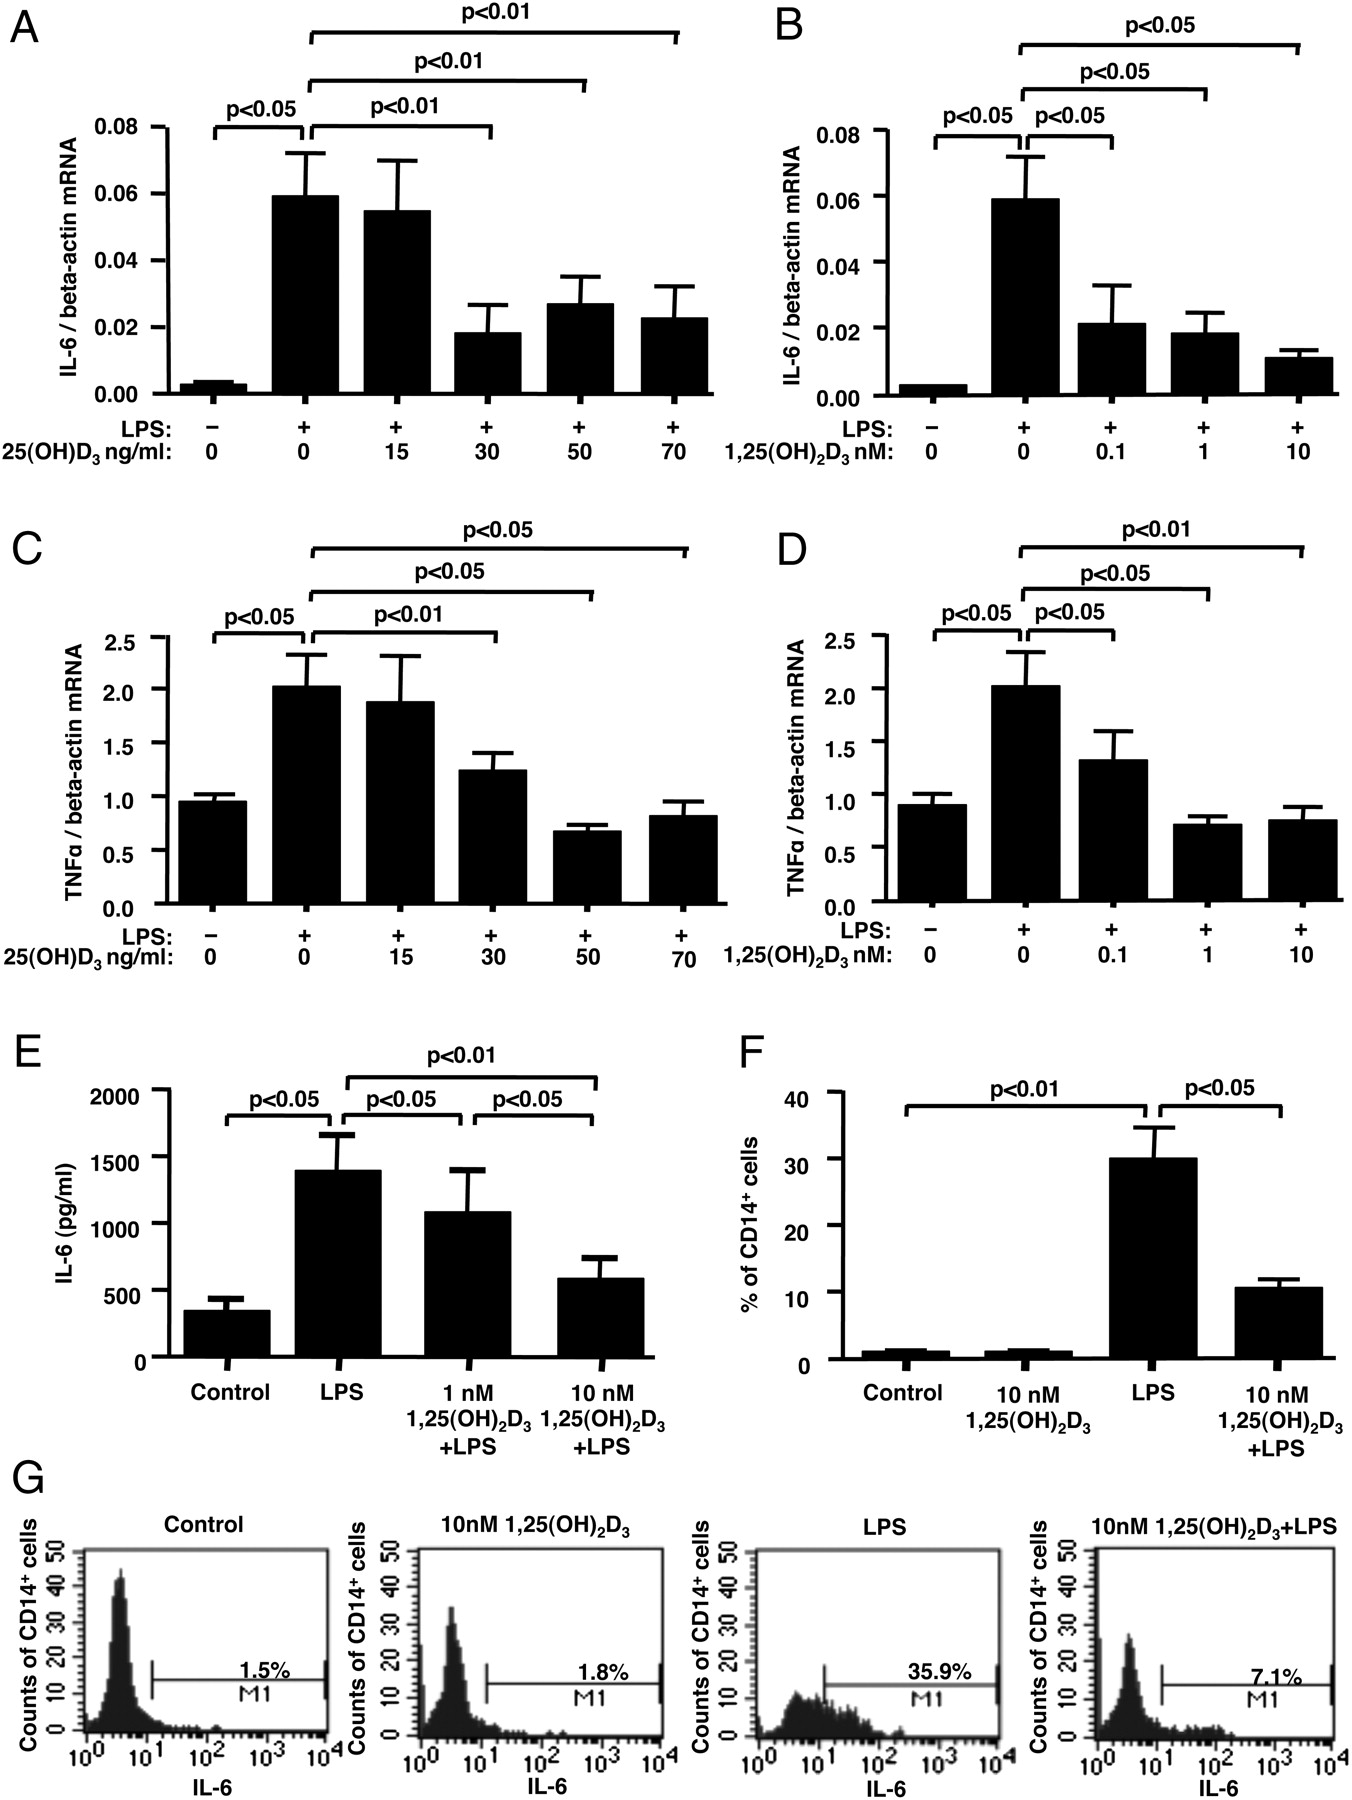
\includegraphics{figures/Zhang.2012-vd_dose_cytokine.jpeg}

}

\caption{\label{fig-vd-dose-cytokine}Effets de la vitamine D sur la
production de cytokines \autocite{Zhang.2012}.}

\end{figure}%

\subsection{Etudes cliniques}\label{etudes-cliniques}

\begin{itemize}
\item
  Au moins 50 ng/mL de vitamine D nécessaire pour une protection contre
  la COVID-19. \textcite{Wimalawansa.2022}
\item
  Infections diminuent lorsque le taux de 25OHD augmente: Association
  between preoperative 25-hydroxyvitamin D level and hospital-acquired
  infections following Roux-en-Y gastric bypass surgery
  https://pubmed.ncbi.nlm.nih.gov/24284777/
\end{itemize}

A strong, inverse association of serum 25(OH)D concentrations \&
COVID-19 severity

\subsubsection{Etude en phase de
prévention}\label{etude-en-phase-de-pruxe9vention}

\begin{itemize}
\tightlist
\item
  \textcite{Sartini.2024}: Méta-analyse sur la prévention par vitamine D
  \textbf{avant} la présence de COVID-19

  \begin{itemize}
  \tightlist
  \item
    7 RCTs : 40\% OR (high heterogeneity)

    \begin{itemize}
    \tightlist
    \item
      5 RCTs on healthcare workers (HCW) = 80\% OR
    \end{itemize}
  \item
    Treatment vs non treatment: OR 0.177, 95\% IC 0.104--0.301

    \begin{itemize}
    \tightlist
    \item
      The odds of the outcome occurring in the treatment group are 0.177
      times (or 82.3\% lower) the odds of the outcome occurring in the
      non-treatment group.
    \end{itemize}
  \item
    2 RCT on non healthcare workers = échec =\textgreater{} low vitD
    dosage

    \begin{itemize}
    \tightlist
    \item
      Oristrell : 3200 IU D3 vs 800 D3 ; 45 vs 55 (intervention vs
      control) ; faible vitamine D
    \item
      Brunvoll: 5 mL of cod liver oil = 400 IU D3/day, 227 vs 228,
      faible vitamine D
    \end{itemize}
  \end{itemize}
\item
  \textcite{Borsche.2021}: La méta-analyse suggère que la vitamine D
  confère une réduction de l'infection, à une concentration débutant à
  partir de 30 ng/mL, optimale à 55 ng/mL.
\end{itemize}

\subsubsection{Etudes en phase curative}\label{etudes-en-phase-curative}

\subsubsection{Etudes en phase
réanimation}\label{etudes-en-phase-ruxe9animation}

1.Leaf, D.E., Raed, A., Donnino, M.W., Ginde, A.A., and Waikar, S.S.
(2014). Randomized Controlled Trial of Calcitriol in Severe Sepsis. Am J
Resp Crit Care \emph{190}, 533--541. 10.1164/rccm.201405-0988oc.

\newpage{}

\chapter{Conclusion}\label{conclusion}

\newpage{}

\hypertarget{Bibliographie}{%
\chapter*{\centering Bibliographie}\label{Bibliographie}}
\addcontentsline{toc}{chapter}{Bibliographie}
\singlespace

\printbibliography[heading=none]




\end{document}
